%% An Introduction to LaTeX Thesis Template of Wuhan University
%%
%% Created by WHUTUG

\documentclass[type=master,class=academic]{whu-thesis}
\whusetup
  {
    info               =
      {
        title          = {基于Inception和混合注意力的运动想象脑电图分类研究},
        % title*         = {An Introduction to LaTeX Thesis Template\\of Wuhan University},
        student-number = {2021202110015},
        school         = {计算机学院},
        author         = {刘梓轩},
        % author*        = {Your Name},
        subject        = {计算机科学与技术},
        major          = {计算机科学与技术},
        advisor        = {李石君 , 教授},
        direction      = {机器学习与应用},
        % date           = {2021/5},
        keywords       = {脑机接口 , 运动想象 , 脑电图 , 注意力 , 深度学习},
        keywords*      = {BCI , Motor Imagery , EEG , attention , Deep Learning},
      },
    style              =
      {
        graphics-path  = {{figures/}{data/}},
        list-of-figures = false,
        list-of-tables = false,
        cite-style = numerical-super,
        bib-style = numerical
      },
    element            =
      {
        innovation     = {pages/innovation},
        abstract       = {pages/abstract},
        abstract*      = {pages/enabstract},
        bibliography   = {ref/refs , ref/thu},
        achievements   = {pages/achievements},
        thanks         = {pages/thanks}
        % appendix       = {pages/appendix}
      }
  }

\begin{document}
%%----------- 主体部分 ----------- %%
% chapter1 绪论

\chapter{绪论}

\section{研究背景及意义}

大脑是一个结构和功能都很复杂的器官,是人体内外环境信息获得、存储、处理、加工及整合的中枢\cite{LXTX201902004},其神经活动蕴含着丰富的信息,直接反映了人类的思维、情绪和行为意图。
对大脑的研究,不仅可以防止大脑的衰退以及脑疾病的产生,而且可以通过模拟大脑促进人工智能的发展\cite{KYYX201907013}。

现今世界,各国政府及科研机构都高度重视脑科学研究的发展,美国于2013年启动“创新性神经技术大脑研究”计划,旨在开发和应用新的工具和技术,彻底改变人类对大脑的理解\cite{jorgenson2015brain}。
日本于2014年启动“脑/思维”计划,研究集中在三个领域:狨猴大脑的结构和功能图谱,用于脑图绘制的创新神经技术,以及人类脑图谱\cite{okano2015brain}。
欧盟于2013年启动“人类脑计划”,最初目标为通过超级计算机对人脑进行模拟,该项目已于2023年9月结束,其在神经科学领域取得了多项重大进展\cite{naddaf2023europe}。
中国于2021年将“脑科学与类脑研究”列为科技创新2030重大项目\cite{china2021brain},正式启动了“中国脑计划”,其内容包括认知神经机制的基础研究,脑疾病诊断和干预的转化研究以及脑启发智能(类脑)技术\cite{POO2016591}。

脑机接口(Brain Computer Interface,BCI)是脑科学与信息科学交叉产生的新兴学科领域,研究如何在大脑与外部设备之间建立直接的通信和控制通道,实现脑与设备之间的双向信息传输。
脑机接口系统的目标是将人类的思维、意愿或行动指令实时转化为可识别的控制信号,从而使人类可以直接由大脑而非神经肌肉通路来控制计算机或设备,
双向脑机接口系统不仅可以实现大脑控制,也为通过神经接口调节中枢神经系统提供了一种可能的方案\cite{he2020brain}。
脑机接口的基础在于采集大脑活动产生的生物信号,例如脑电图(Electroencephalography, EEG)、功能性磁共振成像(Functional Magnetic Resonance Imaging,fMRI)、近红外光谱(Near-Infrared Spectroscopy,NIRS)等,
这些生物信号从不同角度反映了大脑的认知过程、情绪状态和意图表达,其中,脑电图以其实时性、灵活性、便携性、低成本、非侵入性、高时间分辨率等优点,在脑机接口研究领域中受到了广泛的应用。

运动想象(Motor Imagery, MI)是脑机接口研究的主要方向之一,其表征的是一种运动意图,即个体在不实际执行物理动作的情况下,在大脑中想象执行特定动作的一种心理过程。
运动想象的研究源于对大脑功能区域的认知神经科学探索,研究发现,当人们想象执行某个动作时,即使身体并未实际做出该动作,大脑中的特定脑区仍会有所激活。
这种现象为基于运动想象的脑机接口系统提供了理论基础,通过识别和解码运动想象相关的脑电信号,可以基于使用者的自主意识实现对辅助设备的非侵入式控制,
% 其在改善脑卒中患者运动功能障碍\cite{ZKLS202103005},中、重度肢体运动功能障碍患者康复\cite{pichiorri2015brain},智能人机协作,
其在运动功能代偿、运动功能修复\cite{pichiorri2015brain}、智能人机协作、认知神经科学研究、游戏和虚拟现实等领域具有广阔的应用前景。

近年来,随着认知神经科学的持续发展以及各国政府对脑科学的日益重视,运动想象研究领域逐渐吸引了广泛的关注。
在基于脑电图信号进行运动想象分类的研究中,鉴于脑电信号固有的复杂性与异质性,传统机器学习方法通常需要依据神经科学领域的先验知识进行人工特征设计,
随着深度学习的迅速发展,研究者们开始将深度神经网络应用于运动想象分类任务中,期望能够自动化提取和学习脑电图信号中蕴含的潜在特征,
然而,受限于数据集规模、脑电数据质量、实时响应性能等因素,深度学习在该领域的应用效果尚未达到理想的水平。

综上所述,尽管运动想象研究已积累了一系列有价值的科研成果,但是依然存在一定的进步空间。
目前基于脑电图的运动想象分类任务仍然存在以下问题:

(1) 当前方法的实施常受限于多种条件,如特征提取依赖于专业神经科学知识与实践经验,对滤波的特定频率范围处理要求严苛,以及需要较高的电极采样密度。然而,在实际应用如家庭级和个性化的运动想象脑机接口系统中,往往不具备专家校验、标准滤波、高时空分辨率、高计算性能等理想条件,导致在实际场景的普适性上存在局限,应用场景较窄。

(2) EEG信号固有的非平稳性和被试特异性导致现有分类方法在不同个体间的性能表现差异较大,即使在部分被试上达到较高识别精度,但在其他被试上可能显著降低,这阻碍了运动想象分类模型在广泛人群中的稳定应用。因此,仍然需要进一步提升分类方法的精确度、稳健性和一致性,从而在各类被试中获得更为满意的表现,取得较为稳定均衡的性能。

(3) 基于深度学习的运动想象脑电图分类模型通常拥有庞大的参数规模,这在计算资源有限的边缘设备上运行效率低下,影响实时响应性能,从而制约了运动想象脑机接口系统的普及推广。因此,有必要研发对模型的参数量进行精简,以实现性能与效率的优化。

(4) EEG数据集因隐私保护、被试生理心理状态变化等因素,普遍具有规模偏小且样本多样性不足的特点。尽管数据增强是应对小规模数据集的有效策略,但针对具有被试特异性的EEG信号,某些增强方法可能破坏原始信号中蕴含的有价值信息。此外,数据增强过程会加重训练阶段的数据处理压力,延长训练周期,对运动想象脑机接口系统的实时响应性能有所制约。因此,如何在有限的小规模数据集上实现高效且稳定的性能提升,是需要考虑的问题。

\section{国内外研究现状}

不同于常规的时间序列数据,运动想象脑电图数据具有独特的生理学特征,因此,对基于神经科学先验知识进行的特征提取研究进行回顾,
有利于运动想象领域的深度神经网络的设计。因此,本节将从脑电图特征提取和深度神经网络应用两方面来系统性地介绍运动想象领域的国内外研究现状。

\subsection{基于先验知识的运动想象脑电图特征研究现状}

传统机器学习中,对运动想象脑电图信号(MI-EEG)的处理通常分为预处理、特征提取和分类三个主要步骤\cite{altaheri2023deep},其中,分类算法与其它领域内广泛采用的传统机器学习技术类似,
因此,论文主要介绍与MI-EEG信号生理特性相关的预处理技术和特征提取方法的相关研究。

MI-EEG信号的信息密度在不同通道和频段间呈现出显著差异,并且数据的采集极易受到设备、环境、个体生理状态等因素的干扰,从而产生大量噪声,因此,对MI-EEG信号进行预处理是有必要的。
预处理步骤包括一系列操作,例如通道选择(为MI任务选择最有价值的EEG通道)、信号滤波(为MI工作选择最有意义的频率范围)、信号归一化(围绕时间轴对每个EEG通道进行归一化)、
伪影去除(从MI-EEG信号中去除噪声)\cite{altaheri2023deep}、基线矫正(消除EEG数据漂移带来的影响)等。
其中,伪影去除的经典方法是独立成分分析(Independent Component Analysis,ICA)和离散小波变换\cite{sai2017automated}。

MI-EEG信号的特征主要分为三类:时域特征、频域特征和空间域特征\cite{altaheri2023deep},此外,通过对原始数据的进一步加工和转换,可以构建一系列复合特征,如时频特征、时空特征、时频空特征等。

时域特征反映EEG信号随时间变化的特性,其包括均值、方差、标准差、峰度、偏度等统计量,此外,Bo Hjorth提出了一种快速计算时变信号的三个重要特征的方法,即活动性、移动性和复杂性,统称为Hjorth参数\cite{HJORTH1970306},
Luke等人使用卡尔曼滤波来处理EEG信号的不确定性\cite{7448410},考虑到EEG信号具有分形性质,Hsu提出了一种将分形维数和离散小波变换相结合的方法\cite{HSU2010295}。
空域特征反映EEG信号在不同脑电极上的分布情况,共空间模式(Common Spatial Pattern,CSP)是空域特征提取的经典方法,其核心思想是寻找一组最优的空间滤波器,
通过这组滤波器对原始多通道EEG数据进行空间投影,从而最大化两类信号在投影后空间的方差差\cite{wang2006common}。研究者对CSP算法进行了进一步优化,
提出了滤波器组共空间模式(FBCSP)\cite{ang2008filter}、共稀疏空间谱模式(CSSSP)\cite{dornhege2006combined}、共空间谱模式(CSSP)\cite{lemm2005spatio}、小波共空间模式(WCSP)\cite{mousavi2011wavelet}等方法,
在多分类、异步脑机接口等领域取得了更好的效果。
频域特征反映EEG信号在不同频带的功率,通常包括功率谱(Power Spectral)、功率谱密度(Power Spectral Density,PSD)、高阶谱(Higher-order Spectral)、微分熵(Differential Entropy)、傅里叶变换(Fourier Transform)等方法。
Wang等人提出了一种基于快速傅里叶变换(Fast Fourier Transform,FFT)的功率谱特征提取方法\cite{wang2017tinnitus},Kroupi等人使用基于Welch方法的功率谱密度)估计来进行脑电情感分析\cite{kroupi2011eeg},
Herman等人比较分析了不同的频率特征在运动想象分类中的效果,并证实了功率谱密度具有最好的鲁棒性\cite{herman2008comparative}。
时频特征由于结合了时域特征和频域特征,在基于非平稳EEG信号的脑机接口研究中获得了广泛的使用\cite{pawar2020feature},
其主要包括匹配滤波(Matched Filtering,MF)、自回归模型(Autoregressive Model,AR)、短时傅里叶变换(Short-time Fourier Transform,STFT)、小波变换(Wavelet Transform,WT)等方法,时频特征在提升了分类精度的同时,也提高了计算的复杂度。

尽管关于EEG信号特征提取的研究已积累了大量成果,然而传统预处理及特征提取方法仍存在着计算复杂度较高以及信息丢失的可能性,
同时,EEG信号的特征提取高度依赖神经科学领域的先验知识,从而限制了特征提取的自动化程度\cite{altaheri2023deep}。在这种背景下,深度学习被引入运动想象分类领域,
以克服传统方法存在的问题。

\subsection{基于深度学习的运动想象脑电图分类研究现状}

随着深度学习的迅速发展,基于深度学习的方法开始被应用于运动想象脑电图分类任务中,并取得了良好的效果。基于深度学习的运动想象脑电图分类方法主要包括三个部分:数据预处理,网络输入模式,以及深度神经网络架构。

在数据预处理阶段,由于与运动想象相关的脑电图事件相关去同步化(Event-Related Desynchronization,ERD)和事件相关同步化(Event-Related Synchronization,ERS)主要发生在Mu节律(8-12Hz)和Beta节律(18-26Hz)中\cite{altaheri2023deep},多数深度学习方法采用带通滤波技术来提取相关频率成分。然而,这种方法可能会干扰或削减脑电图信号中的有效信息。此外,部分研究通过人工或自动手段去除脑电信号中的伪迹,例如Ma等人\cite{ma2019deep}采用了自动伪迹去除工具箱\cite{gomez2006automatic}。

在网络输入模式方面,研究\cite{luo2018exploring,olivas2019classification,she2019hierarchical,ma2020dwt,chu2018decoding,hassanpour2019novel}使用CSP、FBCSP、PSD、FFT、离散小波变换(Discrete Wavelet Transformation,DWT)等算法进行特征的提取,并将提取的特征作为深度神经网络的输入。然而,这些特征提取算法在一定程度上依赖于神经科学的先验知识和专家经验,并且人工设计的算法可能导致对某些重要信息的遗漏。Xu等人\cite{xu2018wavelet}使用WT算法将脑电图信号转化为频谱图,以更全面地表征时域和频域特征。Miao等人\cite{miao2020spatial}则使用FFT算法获取空频图,表征脑电图信号中的空域特征和频域特征。Li等人\cite{li2020novel}更进一步地将不同通道的数据进行组合,形成了时域、空域、频域的三维表示。尽管将脑电信号转换为图像形式有助于更好地表征EEG信号中不同域的信息,但这也会加剧计算资源的消耗,延长训练的时间。Amin\cite{amin2019deep}等人基于深度学习自动提取特征的概念,将EEG原始数据直接传入深度神经网络中进行训练。近年来,端到端的深度学习网络在运动想象脑电图分类任务中日益受到重视。

对于深度神经网络架构,卷积神经网络(Convolutional Neural Network, CNN)、循环神经网络(Recurrent Neural Network, RNN)等深度网络架构在运动想象脑电信号分类任务中被广泛应用。

卷积神经网络是深度学习中最常见的模型架构之一,擅长捕捉信号的局部特征,并随着网络层次加深逐步提取更高层次的抽象特征。在运动想象分类任务中,CNN不仅可以处理时频图、空频图和时空频三维图等转换后的数据,还可以直接应用于原始EEG数据。Schirrmeister等人\cite{schirrmeister2017deep}提出了一系列基于CNN的网络架构,包括ShallowConvNet和DeepConvNet,它们通过堆叠轴向卷积层替代传统的卷积层,实现了无需预先进行人工特征提取的情况下对脑电信号进行分类。Lawhern等人\cite{lawhern2018eegnet}提出了EEGNet,将深度卷积和可分离卷积引入网络架构中,构建了一种紧凑的通用型模型。Riyad等人\cite{riyad2021mi}在EEGNet的基础上提出了MI-EEGNet,针对运动想象分类任务进行了进一步的改进。Mane等人\cite{mane2021fbcnet}提出了FBCNet,将FBCSP算法的思想融入网络设计中,通过多个窄带滤波器对原始脑电图进行滤波,得到EEG信号的多视图表示。Zhang等人\cite{zhang2021eeg}使用了多个分支进行多尺度的特征提取。Song等人\cite{song2022eeg}为了捕获脑电图信号中的长期依赖关系,将Transformer\cite{vaswani2017attention}模型引入CNN模型之后,直接处理经过一维时间和空间卷积层后的序列。Musallam等人\cite{musallam2021electroencephalography}基于残差神经网络(Residual Network,ResNet)\cite{he2016deep}构建了一种专用于运动想象脑电图分类的模型。Miao等人\cite{miao2023lmda}提出了一种专为脑电图信号解码设计的轻量级注意力模块,对ShallowConvNet和EEGNet进行了改进。

循环神经网络是一类专门设计用于处理序列数据的神经网络架构,它的特点是网络内部包含循环结构或反馈连接,使得信息可以在时间步之间传递和累积,特别适合处理具有时间依赖性或顺序结构的数据。RNN的变体有长短期记忆网络(Long Short-Term Memory,LSTM),门控循环单元(Gated Recurrent Unit,GRU)等。LSTM模型是一种能够学习长期关系的RNN网络,克服了传统RNN的梯度消失问题,其在自然语言处理领域应用广泛,在运动想象任务中,LSTM也被用来处理EEG序列数据,获取其中蕴含的时域信息。Ma等人\cite{ma2018improving}使用滑动窗口对EEG原始数据进行截取从而进行数据增强,随后采用LSTM进行运动想象的分类。Wang等人\cite{wang2018lstm}提出了一种基于一维聚合近似(One Dimension-Aggregate Approximation,1d-AX)的LSTM模型进行运动想象脑电图分类任务。LKumar等人\cite{kumar2019brain}提出了一种使用CSP算法进行特征提取,线性判别分析(Linear Discriminant Analysis,LDA)进行特征约简,支持向量机(Support Vector Machine,SVM)作为分类器的LSTM模型,在GigaDB\cite{cho2017eeg}和BCI Competition IV-1\cite{blankertz2007non}数据集上分别取得了68.19\%和82.52\%的准确率。

\section{研究内容}

针对现阶段运动想象脑电图分类任务中仍然存在的问题,论文的研究目标为基于现有方法提出一种改进的新模型,其应当具有以下特点:

(1) 端到端:只进行很少数据预处理的端到端模型,旨在减轻对神经科学先验知识和专家经验的依赖,简化数据处理步骤,降低计算成本,并拓宽模型在不同应用场景下的适用范围。

(2) 提升分类精度与泛化能力:在现有方法的基础上进一步提高分类精度,确保模型能在多样化的被试群体中都展现出优秀且稳定的性能,无论被试个体的特异性如何,都能获得较为理想的分类效果。
%对高空间分辨率、频率滤波无依赖

(3) 轻量化:具有较少的参数规模,使得模型能够在计算资源有限的边缘设备上高效运行,从而提升实时响应性能,促进运动想象脑电图分类技术在实际应用中的部署与普及。

为了实现研究目标,论文基于现有方法进行改进,

\section{论文组织结构}

论文主要分为以下五个章节:

第一章,绪论。首先介绍了运动想象脑电图分类研究的背景与意义,其次梳理了该领域的国内外研究进展,分别围绕基于神经科学先验知识的运动想象脑电图特征提取研究和基于深度学习方法的运动想象脑电图分类技术研发进行了介绍。最后介绍了论文的研究目标、研究内容以及论文的整体组织结构。

第二章,运动想象脑电图分类和深度神经网络基础。首先介绍了与运动想象脑电图分类任务相关的神经科学基础知识,其次介绍了卷积神经网络、循环神经网络、注意力机制等深度神经网络的相关基础知识,最后介绍了运动想象脑电图分类任务中的一些特殊网络结构。

第三章,基于双分支特征融合和注意力机制的运动想象脑电图分类网络构建。分析了现阶段运动想象脑电图分类任务中仍然存在的问题,并针对这些问题,提出了进一步的改进方法。

第四章,实验结果分析与模型评估。介绍了实验所需的软硬件环境、所使用的运动想象脑电图数据集,以及运动想象脑电图分类任务的评价指标体系。其次介绍了运动想象脑电图数据处理方法,然后依次展开实验过程和结果讨论,包括消融实验、对比试验和跨被试泛化性实验,验证了论文提出的方法在运动想象脑电图分类任务上的有效性。

第五章,总结与展望。对论文研究工作进行了全面总结,分析了所提方法的优点与局限性,并在此基础上提出了未来可能的研究方向和改进策略。
% chapter2 基础

\chapter{运动想象脑电图分类和深度神经网络基础}

\section{脑电生理基础}

\section{深度神经网络基础}

\section{基于深度学习的运动想象脑电图分类基础}

\section{本章小结}
% chapter3 模型

\chapter{基于脑电图信号的运动想象脑电图分类网络构建}

论文前两个章节主要对运动想象脑电图(Motor Imagery Electroencephalography,MI-EEG)分类领域的基础知识以及相关研究做了一定的介绍,并且对该领域仍然存在的问题进行了分析。本章对这些问题进行进一步的探讨,针对这些问题进行了以下研究:

(1) 针对运动想象脑电图分类任务精度有待提升的问题,构建了一种端到端的新模型HIT-Net:首先,以ShallowConvNet模型为基础,引入多尺度并行特征提取模块(Inception模块)\cite{szegedy2015going}、瓶颈层、深度可分离卷积和混合注意力机制,旨在并行提取多尺度时间特征,促进时空特征的深度融合,同时提高模型对重要特征的关注度;其次,在以上模型的基础上,将密集连接引入Inception模块的分支中,以更好地利用EEG信号的局部细节和浅层特征;最后,引入并行多分支的Transformer模块以更好地利用EEG信号的全局信息,并且针对EEG信号信噪比低的特点,引入软阈值模块对Transformer进行改进,从而减少噪声的干扰。

(2) 针对运动想象脑电图分类任务即时响应的需求,对HIT-Net进行了轻量化设计,构建了一种紧凑型端到端模型VSNet:首先,删去参数量较大的Inception模块和Transformer分支,保留网络的其他结构;其次,使用单层的深度可分离卷积替代Inception模块作为时间卷积层,并对瓶颈层进行调整。

(3) 针对运动想象脑电图缺乏标注数据的问题,设计了一种半监督的迁移学习算法:首先,通过ICA算法和Wasserstein距离\cite{rubner2000earth}选择与目标域分布相似的N个源域;其次,将源域与目标域的特征在黎曼流形上对齐并映射到切线空间,并通过源域与目标域特征的相似性计算特征的权重;最后,基于MEKT算法获取特征映射矩阵,并通过加权投票获取最终的结果。

本章分三个部分对这些研究进行介绍。

\section{基于Inception和混合注意力融合改进的端到端MI-EEG分类网络HIT-Net}

原始的EEG信号通常为二维数据,包括通道(电极)和时间两个维度,具体而言,在EEG信号矩阵中,行代表分布在头皮不同位置的采样通道,列为时间序列数据,每个采样点对应一个时间戳下的生物电信号(通常为电压值),因此,一列数据就是一个特定时间点下所有通道同步采集到的电压读数。原始的EEG信号经过预处理之后,可以转换为时频图、头皮点位拓扑图等输入模式,尽管经过转换的输入相较于原始输入能够更全面地体现EEG信号的时频空信息,但这一过程往往需要具有神经科学背景的人工参与,在增加了人工成本同时,限制了模型自适应学习EEG信号中蕴含的复杂时空特征的能力,此外,复杂的预处理环节也增加了计算开销和应用成本,难以满足BCI系统即时响应的需求。因此,端到端网络在MI-EEG分类领域受到越来越多的重视,这类网络不经过或者仅仅经过很少的预处理步骤,而由深度学习算法自适应地提取关键特征并作出预测。

为此,论文构建了基于Inception和混合注意力融合改进的端到端MI-EEG分类网络HIT-Net(HybridAttention-Inception-Transformer-MI-EEGNet),其结构如图~\ref{fig:HIT}~所示。HIT-Net有两条并行分支,分别是卷积神经网络分支与Transformer分支。卷积神经网络分支基于Inception结构搭建,通过在Inception分支引入密集连接结构,进行多尺度特征提取,同时利用高级语义信息与浅层特征;通过引入反转瓶颈层,在深度维度上促进时空特征的融合,同时通过深度可分离卷积等方法减小网络的参数规模;通过引入svSE混合注意力模块促进网络对重要特征的关注度,svSE模块采取时空特征分离的策略,同时利用了EEG信号的方差信息,以获得针对性的结果。Transformer分支用以获取全局上下文信息,同时采用了时空特征分离的策略,以并行分支方式进行通道上的时间长距依赖信息;通过引入软阈值函数以抑制噪声。卷积神经网络分支与Transformer分支通过CT-Block与TC-Block进行特征的融合,以同时利用Transformer提取的全局信息与卷积神经网络提取的局部细节,构建长短依赖的混合注意力机制。

通过HIT-Net,可以更完整地获取MI-EEG信号的有效特征,提升分类效果。在下文中,将依次阐述论文的改进思路与构建方法。

\begin{figure}
    \centering
    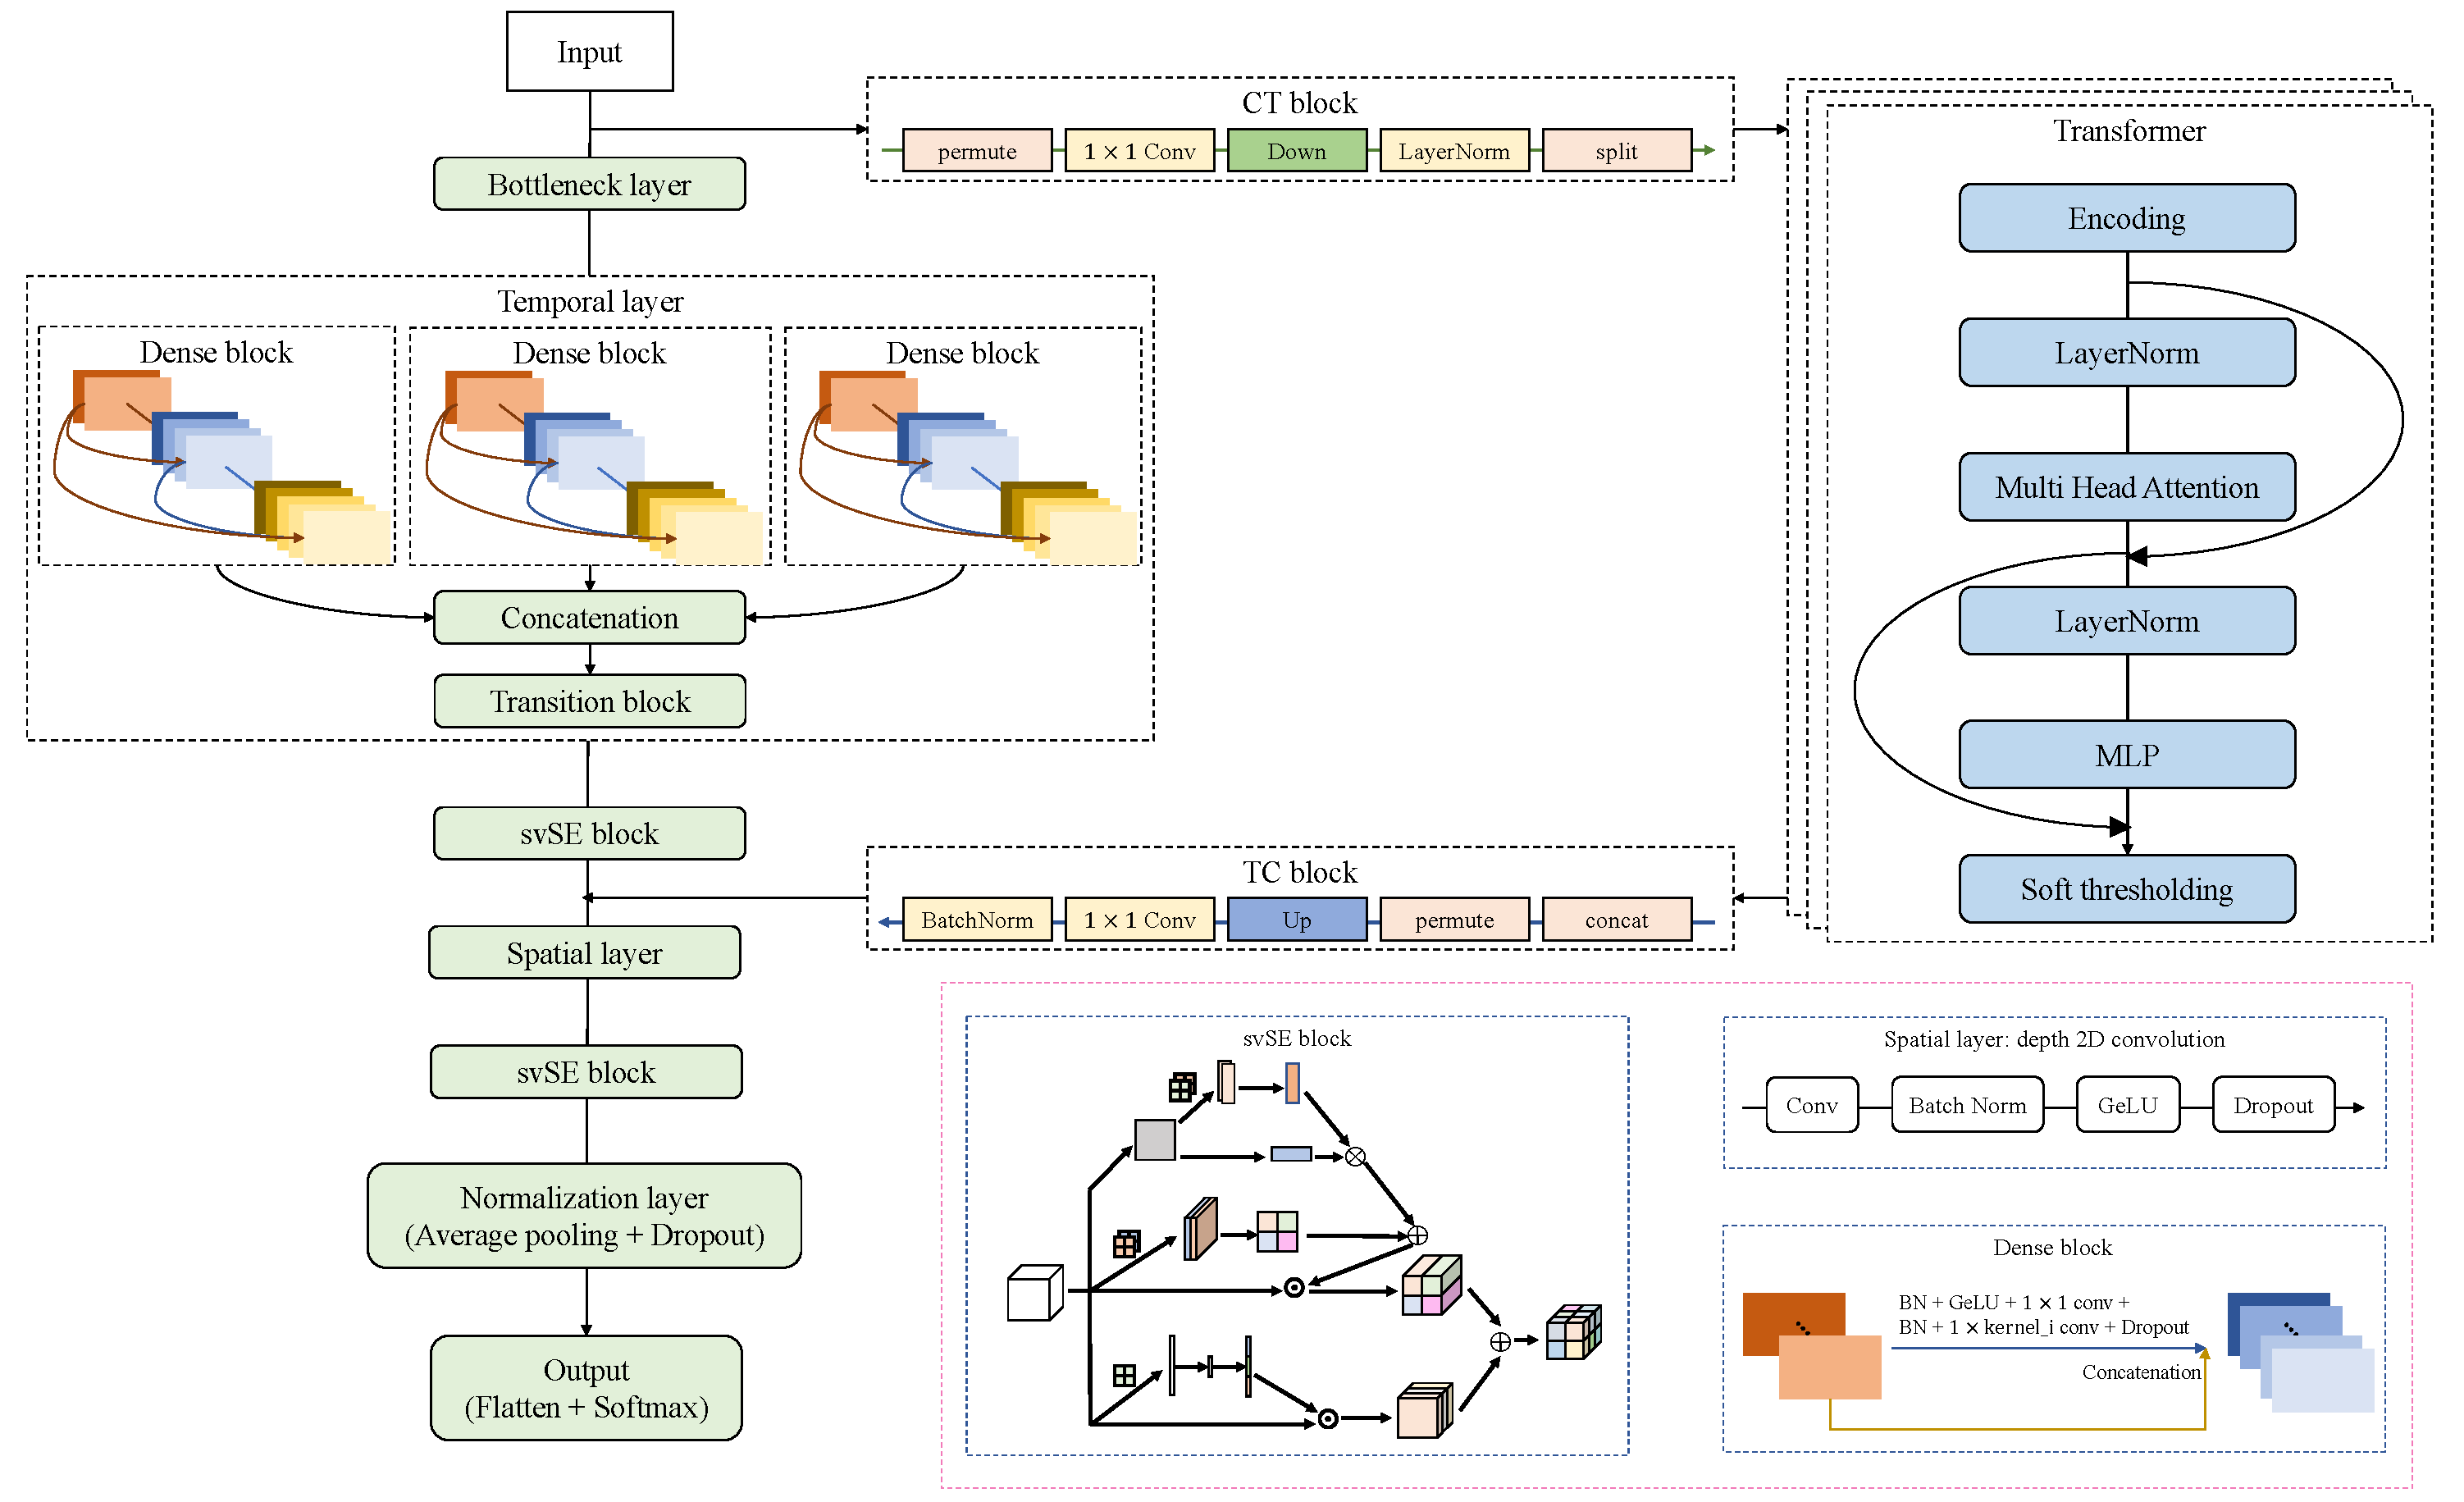
\includegraphics[width=\textwidth]{HIT-Net.pdf}
    \caption{HIT-Net结构}
    \label{fig:HIT}
\end{figure}

\subsection{基础网络BaseNet}

ShallowConvNet\cite{schirrmeister2017deep}是一个专为端到端解码脑电图(EEG)信号而设计的深度学习架构,其构思源自EEG信号解码研究领域中广泛使用的经典特征提取方法——滤波器组共空间模式(Filter Bank Common Spatial Pattern, FBCSP)\cite{ang2008filter}。ShallowConvNet具有FBCSP算法对频带功率特征高效提取的特性,在实验中证明了能够学习频带功率变化的时间结构特性\cite{schirrmeister2017deep},研究发现,该特性有助于提高分类性能\cite{sakhavi2015parallel}。实验证明,ShallowConvNet在MI-EEG分类领域具有优良的性能\cite{lawhern2018eegnet},同时具有较少的参数量,因此论文参考ShallowConvNet设计MI-EEG分类网络。

ShallowConvNet的结构如图~\ref{fig:ShallowConvNet}~所示。ShallowConvNet采用四步流程对原始二维输入数据进行处理。具体而言,ShallowConvNet首先通过时间卷积层捕获信号的时间域特征,再通过空间卷积层捕获这些时间特征在不同通道间的空间关联性,随后通过平均池化层进行下采样,最后通过全连接层将多维特征映射至分类输出空间。ShallowConvNet采取的时间卷积和空间卷积相分离的策略有效地减少了模型参数量,同时,空间卷积核能够学习其对应的时间卷积核提取的特征,这种设计隐含了对FBCSP算法核心思想的借鉴与实现。
\begin{figure}
    \centering
    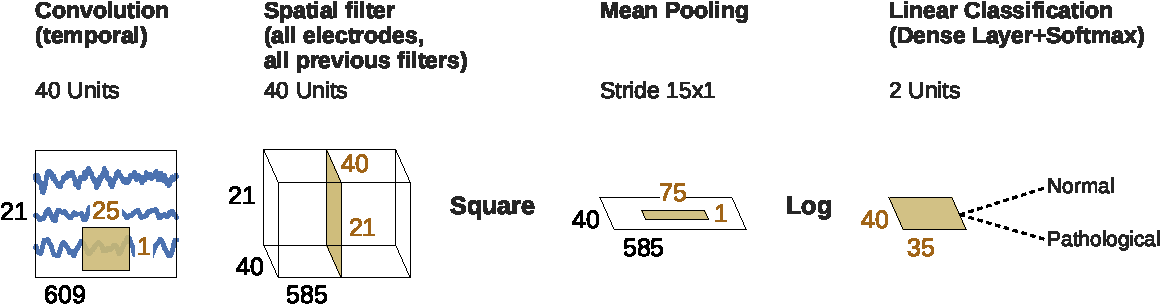
\includegraphics[width=\textwidth]{ShallowNet.pdf}
    \caption{ShallowConvNet结构}
    \label{fig:ShallowConvNet}
\end{figure}

由于EEG原始输入具有时间和通道两个维度的信息,可以被视为具有空间信息的图像数据,因此,论文参考以下几种计算机视觉领域的经典模型,用于网络的特征提取基础结构:

(1) Inception网络

Inception模块起源于经典的GoogLeNet模型\cite{szegedy2015going},并在计算机视觉图像分类任务中取得了优异的效果。传统卷积神经网络倾向于通过加深和拓宽网络结构以增进性能,然而这种做法伴随着参数数量的激增,不仅加大了计算负担,还可能导致过拟合问题。在这种背景下,Inception模块提出了多尺度特征并行抽取的策略,旨在保持网络稀疏性的同时,充分利用密集矩阵运算的高性能。典型的Inception-V1模块的结构如图~\ref{fig:Inception}~所示,其将不同大小的卷积层和最大池化层并行排列,并行地对输入数据执行多种卷积和池化运算,继而将提取到的不同尺度特征在深度维度上进行拼接。这种设计能够在单层网络内并行地提取输入数据在不同层次和粒度的特征信息,从而在高效扩展网络的深度和宽度的同时,有效削减参数规模,提升计算速度。此外,Inception模块中引入了1\times1卷积核,用以实现深度上的特征转化和降维,这种方式能够让模型学习到更为丰富的特征,同时降低计算成本。后续的论文中,Inception模块不断迭代优化,陆续引入了批归一化、深度可分离卷积、矩阵因子分解等技术,进一步提升了模型的性能\cite{szegedy2016rethinking}\cite{szegedy2017inception}。
\begin{figure}
  \centering
  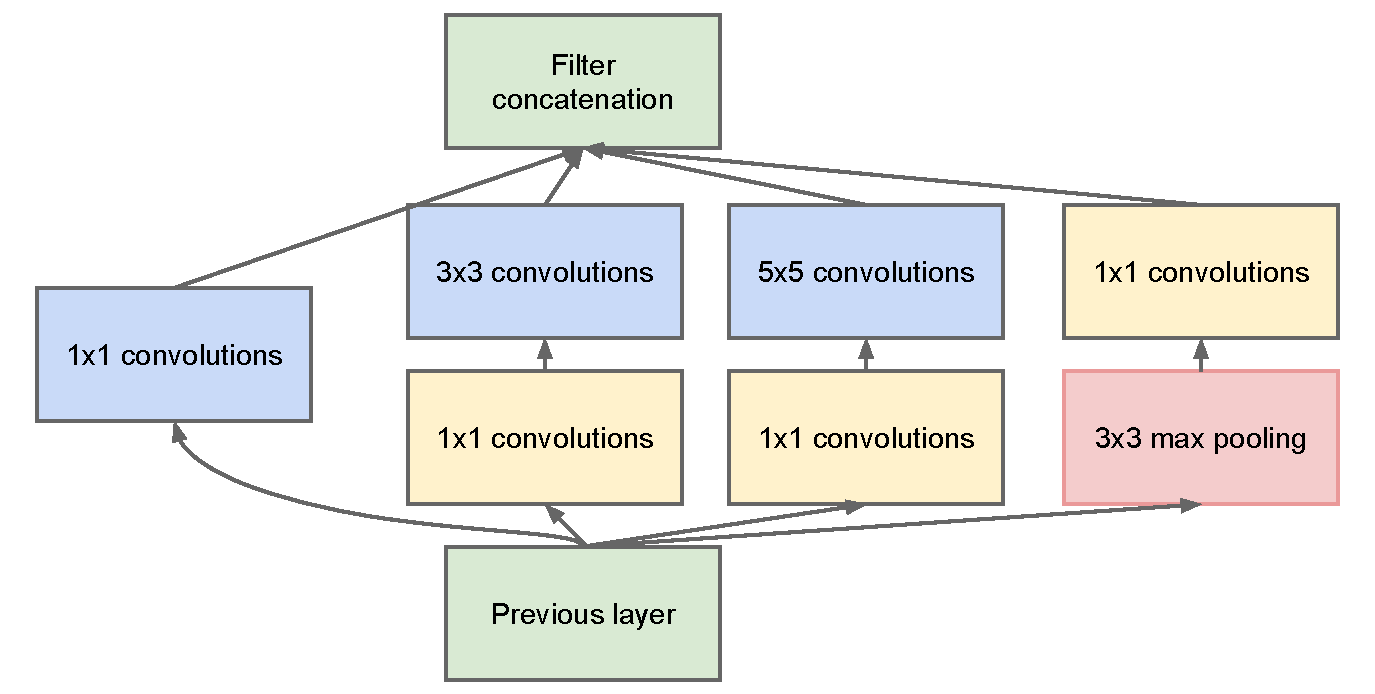
\includegraphics[width=\textwidth]{Inception.pdf}
  \caption{Inception结构}
  \label{fig:Inception}
\end{figure}

(2) 残差神经网络

残差神经网络(Residual Network,ResNet)\cite{he2016deep}是计算机视觉图像识别领域的一个经典模型。ResNet研究发现了深度神经网络的退化现象(Degradation),即随着网络深度不断增加,模型准确率起初随深度上升,却在达到峰值后急剧下滑。针对这种现象,ResNet提出了残差学习框架,其核心思想是引入残差块(Residual Block),每个残差块通过快捷连接(Shortcut Connection)将输入信息直接输送至输出层,使得网络只需要专注学习输入与输出之间的残差信息,而非完整的映射关系。基础的ResNet由一系列残差块堆叠而成,残差块的结构如图~\ref{fig:ResNet}~所示。通过快捷连接,ResNet在训练过程中,梯度能够从深层网络直接回传至浅层,避免网络深度增加带来的训练困难和性能下降问题,从而提升深度神经网络的性能表现和训练效率。
\begin{figure}
  \centering
  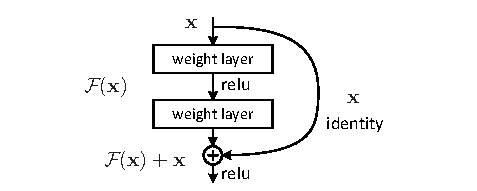
\includegraphics[width=\textwidth]{ResNet.pdf}
  \caption{残差块结构}
  \label{fig:ResNet}
\end{figure}

(3) U-Net

U-Net模型\cite{ronneberger2015u}最初是为生物医学图像分割任务而设计,其具有优秀的性能,尤其在细胞、器官和病变区域的精确标注上表现出色,是医学图像分割领域的主流模型之一。U-Net的独特之处在于其采用了对称的编码-解码结构(Encoder-Decoder)和跳跃连接(skip connection),其结构如图~\ref{fig:UNet}~所示。编码器通过连续的卷积和下采样层对输入图像进行深度特征提取和空间压缩,提炼出高级抽象特征;解码器部分则通过上采样和卷积恢复到与输入图像相同的空间分辨率,同时保留详细的定位信息。跳跃连接将编码器各阶段的特征图直接传递给相应的解码器阶段,有效地结合了包含更多细节信息的浅层特征和包含更多高级语义信息的深层特征,从而在图像分割任务中能够取得更为精细的分割效果。同时,U-Net模型结构简单,易于训练,能够缓解小样本数据集上的过拟合问题。
\begin{figure}
  \centering
  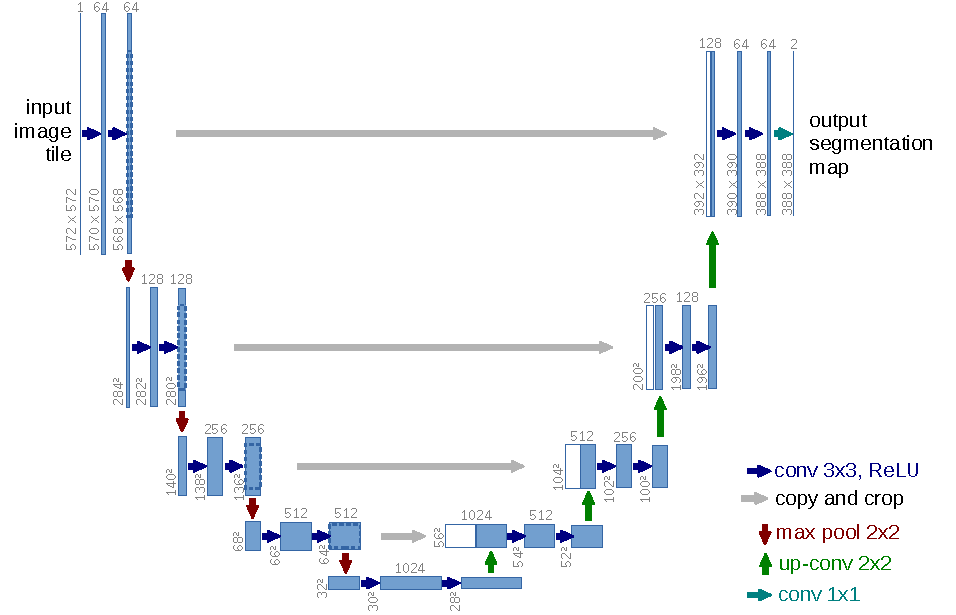
\includegraphics[width=\textwidth]{UNet.pdf}
  \caption{U-Net结构}
  \label{fig:UNet}
\end{figure}

在这三种模型中,Inception和ResNet均在图像分类任务中展现出了优秀的性能。Inception通过同一层网络内的多尺度特征并行抽取,在不显著增加网络深度的前提下,实现了特征提取的广度与效率的提升。ResNet通过引入快捷连接,解决了深度神经网络训练过程中的梯度消失和退化问题,增强了深层次网络的训练效率和性能表现。U-Net则在生物医学图像分割领域取得了优秀的表现,医学图像的语义信息较为简单,且结构较为固定,因此高级语义信息和低级特征都相对重要,U-Net通过跳跃连接保留并融合了这两类信息,同时,U-Net参数量较小,不容易在小样本数据集上发生过拟合现象。论文选择将U-Net迁移至MI-EEG分类任务中,是因为EEG信号具有与生物医学图像类似的生理特性,如特征相对简单、数据集规模偏小等。

为了验证Inception、ResNet与U-Net在EEG信号分类任务中的性能,论文在BCI Competition IV Dataset 2A数据集上进行实验对比。在实验设置中,统一将三种模型的网络深度调整为三层,并对其他关键参数如卷积核大小、学习率等进行了固定,此外,对这三种模型的原始代码进行了调整,使得其适应MI-EEG分类任务。实验结果如表~\ref{tab:Incep-Res-U}~所示,主要展示准确率(Accuracy,ACC)和Kappa一致性系数(Kappa)指标,这两项指标是数据集中九位受试者的平均表现。
\begin{table}[ht]
  \centering
  \caption{Inception、ResNet、U-Net实验结果对比}
  \label{tab:Incep-Res-U}
  \begin{tabularx}{\textwidth}{CCC}
    \toprule
    Models & ACC(\%) & Kappa \\
    \midrule
    Inception & \textbf{67.40} & \textbf{0.56} \\
    ResNet & 56.94 & 0.43 \\
    U-Net & 62.27 & 0.50 \\
    \bottomrule
  \end{tabularx}
\end{table}

实验数据显示,Inception模型在这三种模型中具有最优的性能表现,U-Net次之,ResNet的表现则相对较差。这可能是因为同样的网络深度下,Inception模型得益于多尺度并行特征提取机制,能更全面地捕获EEG信号的多种特征。相比之下,U-Net虽然通过跳跃连接有效地结合了EEG信号的低层特征和高层语义信息,但在解码器阶段,U-Net将特征图重建至原始空间尺寸的过程可能为分类任务引入了不必要的复杂性。ResNet的快捷连接在较浅层网络结构中可能未能完全发挥其优势,更适用于深层次网络。实验结果与过往研究中关于浅层网络更适合MI-EEG分类任务的研究结论相互印证。综上所述,论文选用Inception模块作为MI-EEG信号特征提取的基础结构,旨在保持模型简洁高效的同时,在MI-EEG分类任务中取得更好的性能。

EEG信号的空间特征复杂度通常低于时间特征复杂度,时空信息具有不均衡性。例如,在BCI Competition IV Dataset 2B\cite{tangermann2012review}数据集中,仅仅使用了三个电极采集MI-EEG信号,使得空间信息相对时间信息更为稀疏。因此,论文采取更关注时间特征的策略,即将Inception模块应用于时间卷积层中,使得时间卷积层的复杂度要高于空间卷积层的复杂度,这一策略的目的在于使得模型具有捕捉高维时空特征能力的同时,防止模型因复杂度过高而在小样本数据集上过早地发生过拟合现象。

空间卷积层有两种不同的方式融入基于Inception改进的时间卷积层之后,一种是在每个Inception模块内部的分支结构上增加空间卷积层,另一种则是在整个Inception模块之后附加空间卷积层。图~\ref{fig:ts-incep}~展示了这两种引入方式的区别,将这两种方式分别称为分支内融合(Inception-In)和模块后融合(Inception-After),需要说明的是,图中省略了网络的其他结构,如瓶颈层等,以尽可能简洁地展现不同引入方式的差异。
\begin{figure}
  \centering
  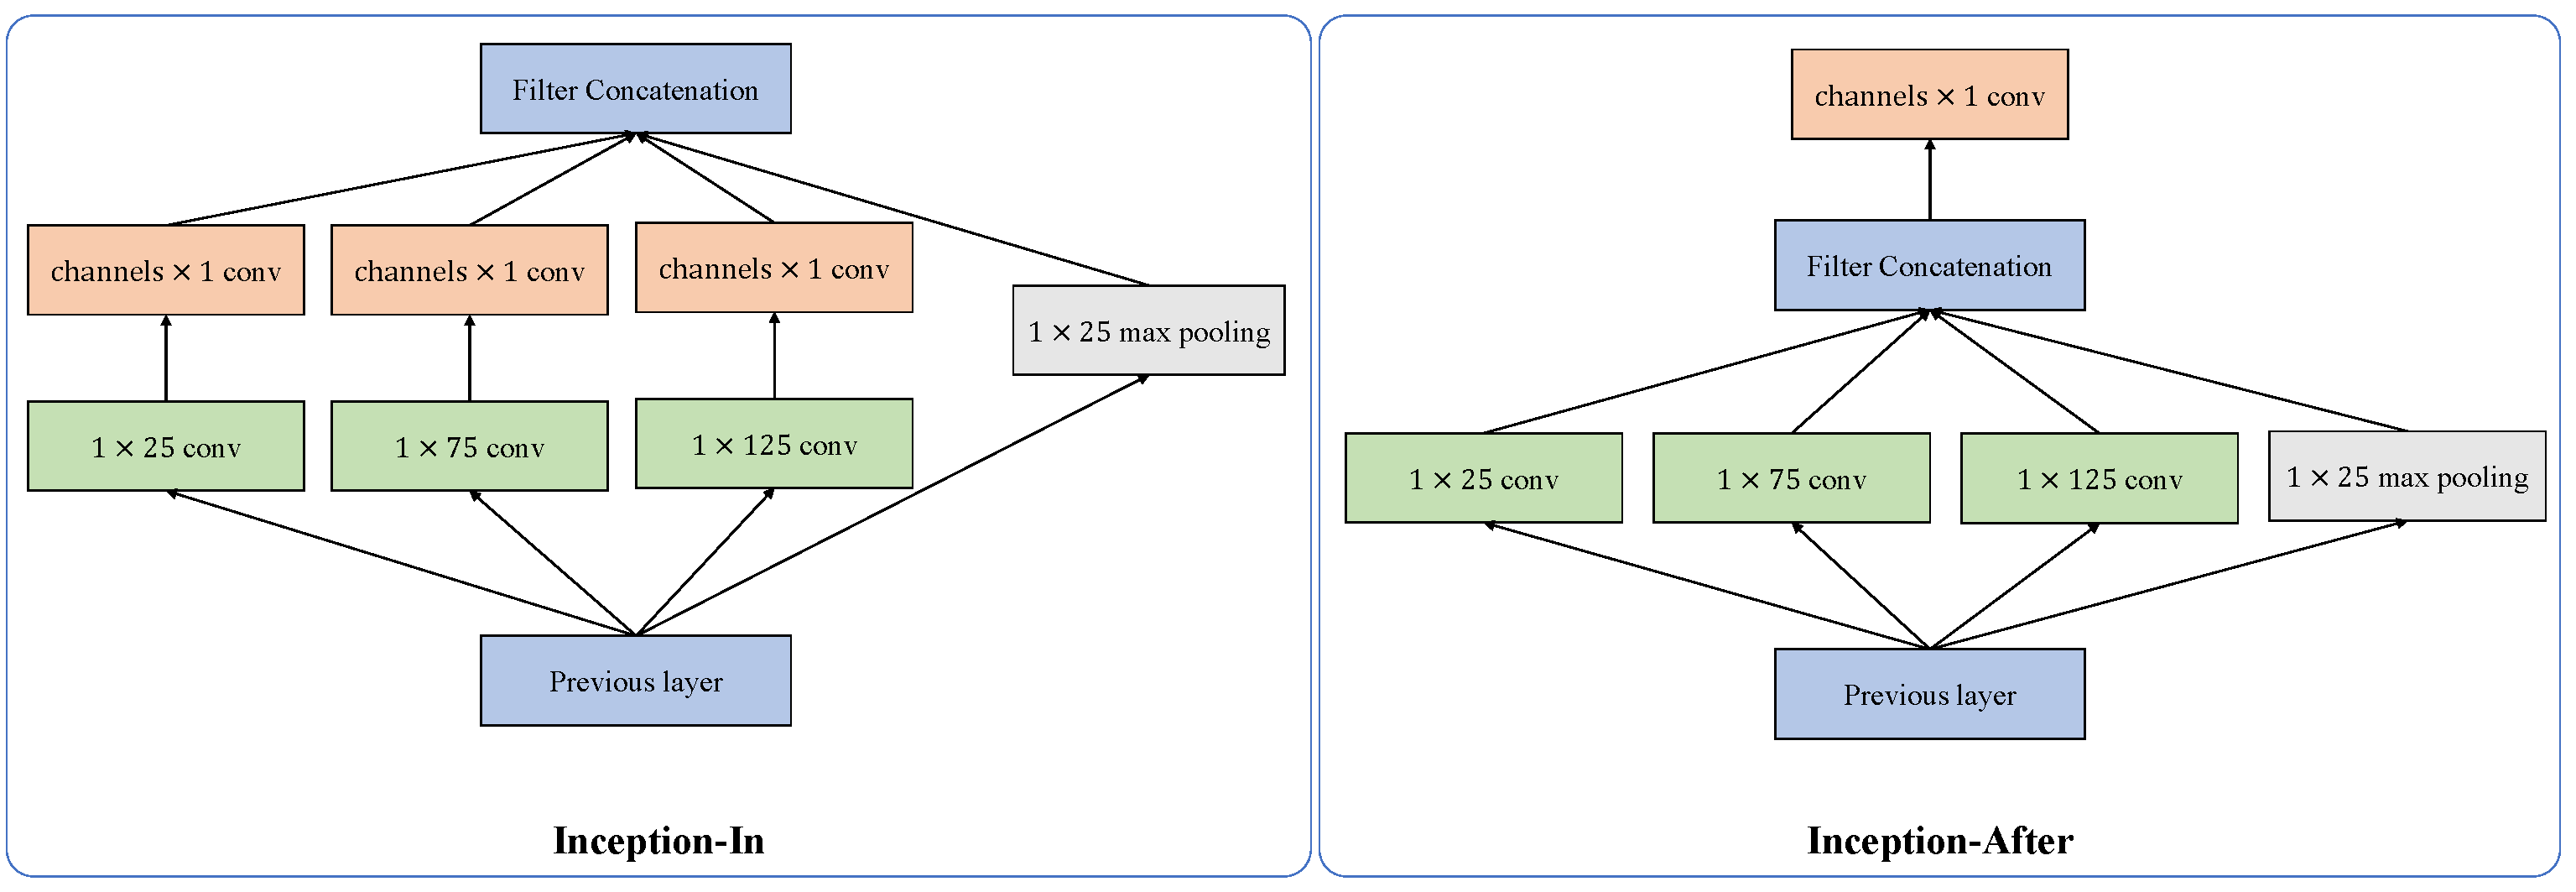
\includegraphics[width=\textwidth]{ts-incepv2.pdf}
  \caption{Inception模块引入空间卷积层的方式}
  \label{fig:ts-incep}
\end{figure}

为了比较Inception-In与Inception-After的性能差异,论文在BCI Competition IV Dataset 2A数据集上设计实验进行对比。在实验设置阶段,固定了Inception模块的层次数量、分支数量等参数,实验结果如表~\ref{tab:ts-inception}~所示。在此,重点关注两项评价指标——准确率(Accuracy, ACC)和Kappa一致性系数(Kappa),这两项指标均基于数据集中九位受试者的平均表现。实验结果显示,Inception-After方式在准确率和一致性系数上均表现更优。这一优势可能源自两方面的原因:一方面,虽然Inception-In模式借鉴了FBCSP算法的分频段处理思路,但在Inception分支内部直接进行空间特征提取的过程中,损失了部分空间全局信息;另一方面,Inception-In结构具有相对更大的参数规模,这可能导致模型在有限样本条件下更容易出现过拟合现象。基于以上分析和实验验证,论文选择以Inception-After的方式布局时间卷积层与空间卷积层。
\begin{table}[ht]
  \centering
  \caption{Inception-In、Inception-After实验结果对比}
  \label{tab:ts-inception}
  \begin{tabularx}{\textwidth}{CCC}
    \toprule
    Models & ACC(\%) & Kappa \\
    \midrule
    Inception-In & 63.31 & 0.51 \\
    Inception-After & \textbf{75.35} & \textbf{0.70} \\
    \bottomrule
  \end{tabularx}
\end{table}

文献\cite{lawhern2018eegnet}\cite{schirrmeister2017deep}指出,在EEG信号解码任务中,增加神经网络的深度有利于提升解码精度。瓶颈层(Bottleneck Layer)是深度神经网络中的常见结构\cite{he2016deep}\cite{huang2017densely},通常用于对数据的降维和升维,由于采用了1\times1卷积进行操作,瓶颈层能够有效地减少神经网络的参数。不同于原始Inception模块中通过瓶颈层进行数据降维的操作,论文使用瓶颈层对数据进行升维操作,并将瓶颈层提取至卷积和池化操作之前,其目标为在深度维度上促进时空信息的融合。

为了加快网络训练速度,并避免小数据集下过早的过拟合,论文在引入瓶颈层的基础上,对网络的结构进行了进一步的调整:

(1) 借鉴EEGNet\cite{lawhern2018eegnet}的结构,将时间卷积和空间卷积替换为参数量更少的深度可分离卷积\cite{lawhern2018eegnet};

(2) 在模型中引入了一系列正则化技术,包括批量归一化(Batch Normalization,BN)和随机Dropout等。

此外,论文将ShallowConvNet中的对数激活函数替换为GELU激活函数,前者基于FBCSP算法中的对数方差计算提出,后者基于高斯分布和自然梯度流提出,能够更自然地模拟神经元的概率行为,具有更好的连续性和光滑性\cite{hendrycks2016gaussian},实验证明了GELU激活函数较之对数激活函数具有更好的效果。

论文将改进后得到的基础模型称为BaseNet,其结构如图~\ref{fig:BaseNet}~所示。需要注意的是,Inception模块的层次数量和分支数量是影响其性能表现的两项可调的超参数。
\begin{figure}
    \centering
    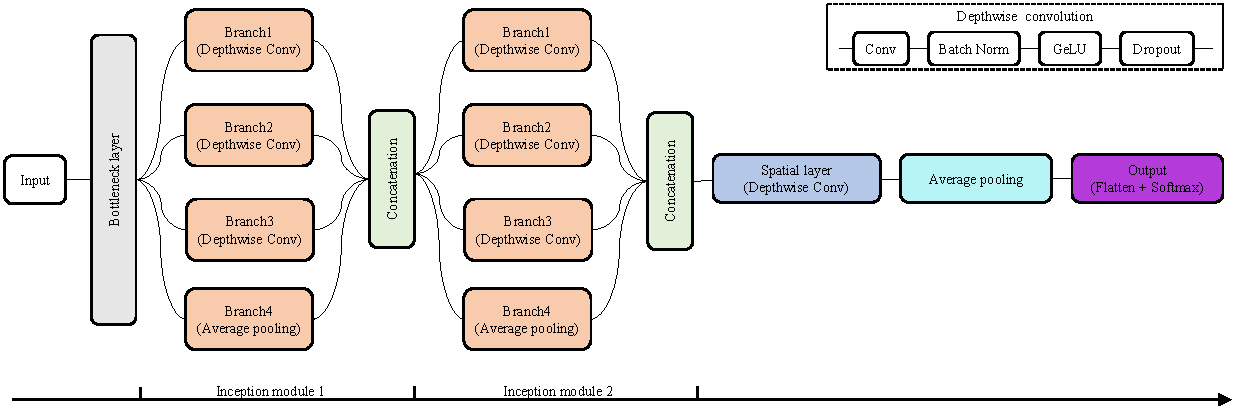
\includegraphics[width=\textwidth]{Base-Net.pdf}
    \caption{BaseNet结构}
    \label{fig:BaseNet}
\end{figure}

\subsection{局部混合注意力svSE}

注意力机制的提出受到人类认知科学的启发,其核心理念在于模拟人类大脑在处理信息过程中的选择性关注机制,即并非均匀地分配注意力处理对待所有输入,而是将注意力主动、动态且有选择性地聚焦于最重要或最相关的信息上。自二十世纪被提出以来\cite{730558},注意力机制在计算机视觉、自然语言处理等领域得到了广泛的应用,并表现出了优秀的效果。根据神经科学先验知识,EEG信号中不同的通道和采样点具有不同的重要性,这为在MI-EEG分类领域应用注意力机制提供了理论依据,此外,将二维EEG信号视为一种由通道和时间两个维度构成的特殊图像,使得在MI-EEG分类领域能够迁移应用计算机视觉领域中的注意力机制。

计算机视觉领域中经常使用的注意力机制有:

(1) 通道注意力机制
    
不同于EEG信号中代表电极的通道,计算机视觉领域的通道代表图像的不同特征映射。通道注意力机制用于调整不同特征通道的重要性,通常会对每一个特征通道计算一些全局统计量,如均值、方差等,再将这些统计量经过非线性变换层进行编码,最后将编码向量进行转换并用于各个特征通道的加权。通道注意力机制的经典模型是压缩和激励网络(Squeeze-and-Excitation Networks,SENet)\cite{8578843},其主要思想即是压缩(Squeeze)和激励(Excitation),SENet首先通过压缩操作获取全局上下文信息,然后通过激励操作对每个通道独立生成权重系数。具体而言,在压缩操作中,SENet在空间维度执行全局池化操作,将每个通道的特征图汇总成一个标量值;然后,在激励操作中,SENet通过一个全连接网络生成每个通道的权重系数,这些权重系数用于重新加权每个通道的特征图,以增强有用的特征并抑制无用的特征。

在后文中,为避免与计算机视觉领域中的概念相混淆,在MI-EEG分类任务中,用深度来代表EEG信号的不同特征映射,而通道仍然代表电极。

(2) 空间注意力机制
    
在计算机视觉领域中,空间注意力机制用于调整图片、视频等输入数据在空间维度中不同区域的重要性,通常会在深度维度上通过全局池化、卷积、特征融合等操作生成一个与特征图尺寸相同的注意力图,其值反映了空间维度中不同区域的注意力强度,最后,将注意力图进行转换,并用于原始特征图的加权。空间注意力机制的经典模型是空间变换网络(Spatial Transformer Network,STN)\cite{jaderberg2015spatial},其具有对输入数据进行空间变换的能力,能够自动捕获重要区域的特征。

(3) 混合注意力机制
    
混合注意力机制是一种集成多种注意力机制(如空间注意力、通道注意力及自注意力等)的方法,旨在更全面地捕获和整合输入数据在不同维度的有效信息。混合注意力机制通常会使用不同的注意力机制分别计算原始特征图的注意力权重,再将这些注意力权重进行融合,最后将融合后的注意力权重用于原始特征图的加权,或者将不同的注意力权重用于原始特征图加权,再将加权特征图进行融合。混合注意力机制的经典模型有卷积注意力机制模块(Convolutional Block Attention Module,CBAM)\cite{woo2018cbam}、空间与通道压缩与激励模块(Spatial and Channel Squeeze-and-Excitation,scSE)\cite{roy2018concurrent}等。
    
CBAM结合了通道注意力机制与空间注意力机制,其结构如图~\ref{fig:CBAM}~所示,输入特征图首先经过通道注意力模块进行加权,再通过空间注意力模块进行加权,从而得到最终结果。
\begin{figure}
    \centering
    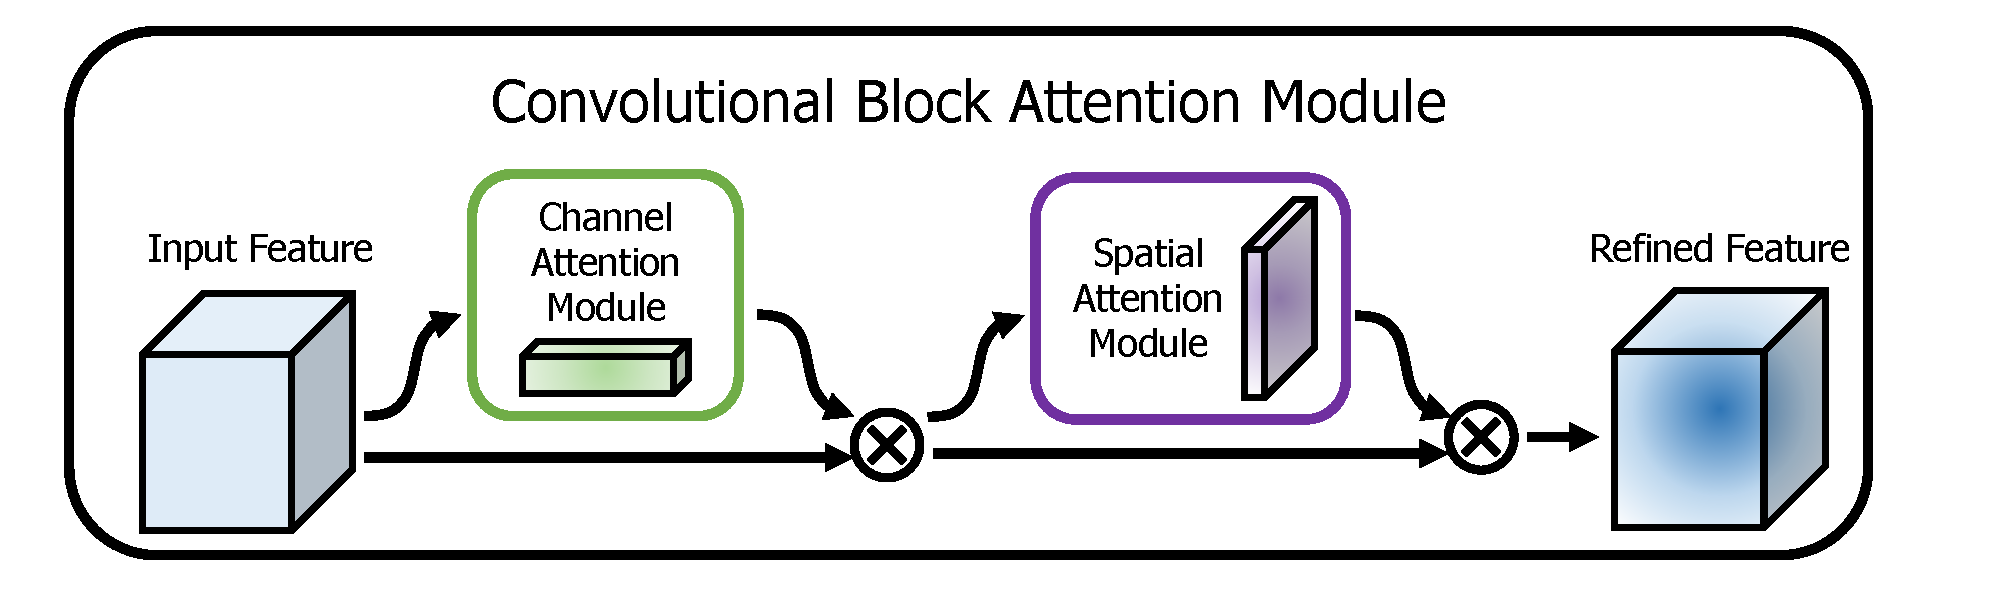
\includegraphics[width=\textwidth]{CBAM.pdf}
    \caption{CBAM结构}
    \label{fig:CBAM}
\end{figure}

具体而言,在通道注意力模块中,输入特征图分别进行空间维度上的全局最大池化和全局平均池化,再将得到的统计值分别通过一个共享权重的全连接层,最后经过逐点加和与非线性变换得到通道注意力权重,用于输入特征图的加权。空间注意力模块的输入是经过通道注意力加权的特征图,首先在通道维度上进行全局最大池化和平均池化,再将得到的统计值在通道维度进行拼接,最后经过卷积降维与非线性变换得到空间注意力权重,与特征图加权后得到最终结果。CBAM的模块结构如图~\ref{fig:CBAM-Block}~所示。
\begin{figure}
  \centering
  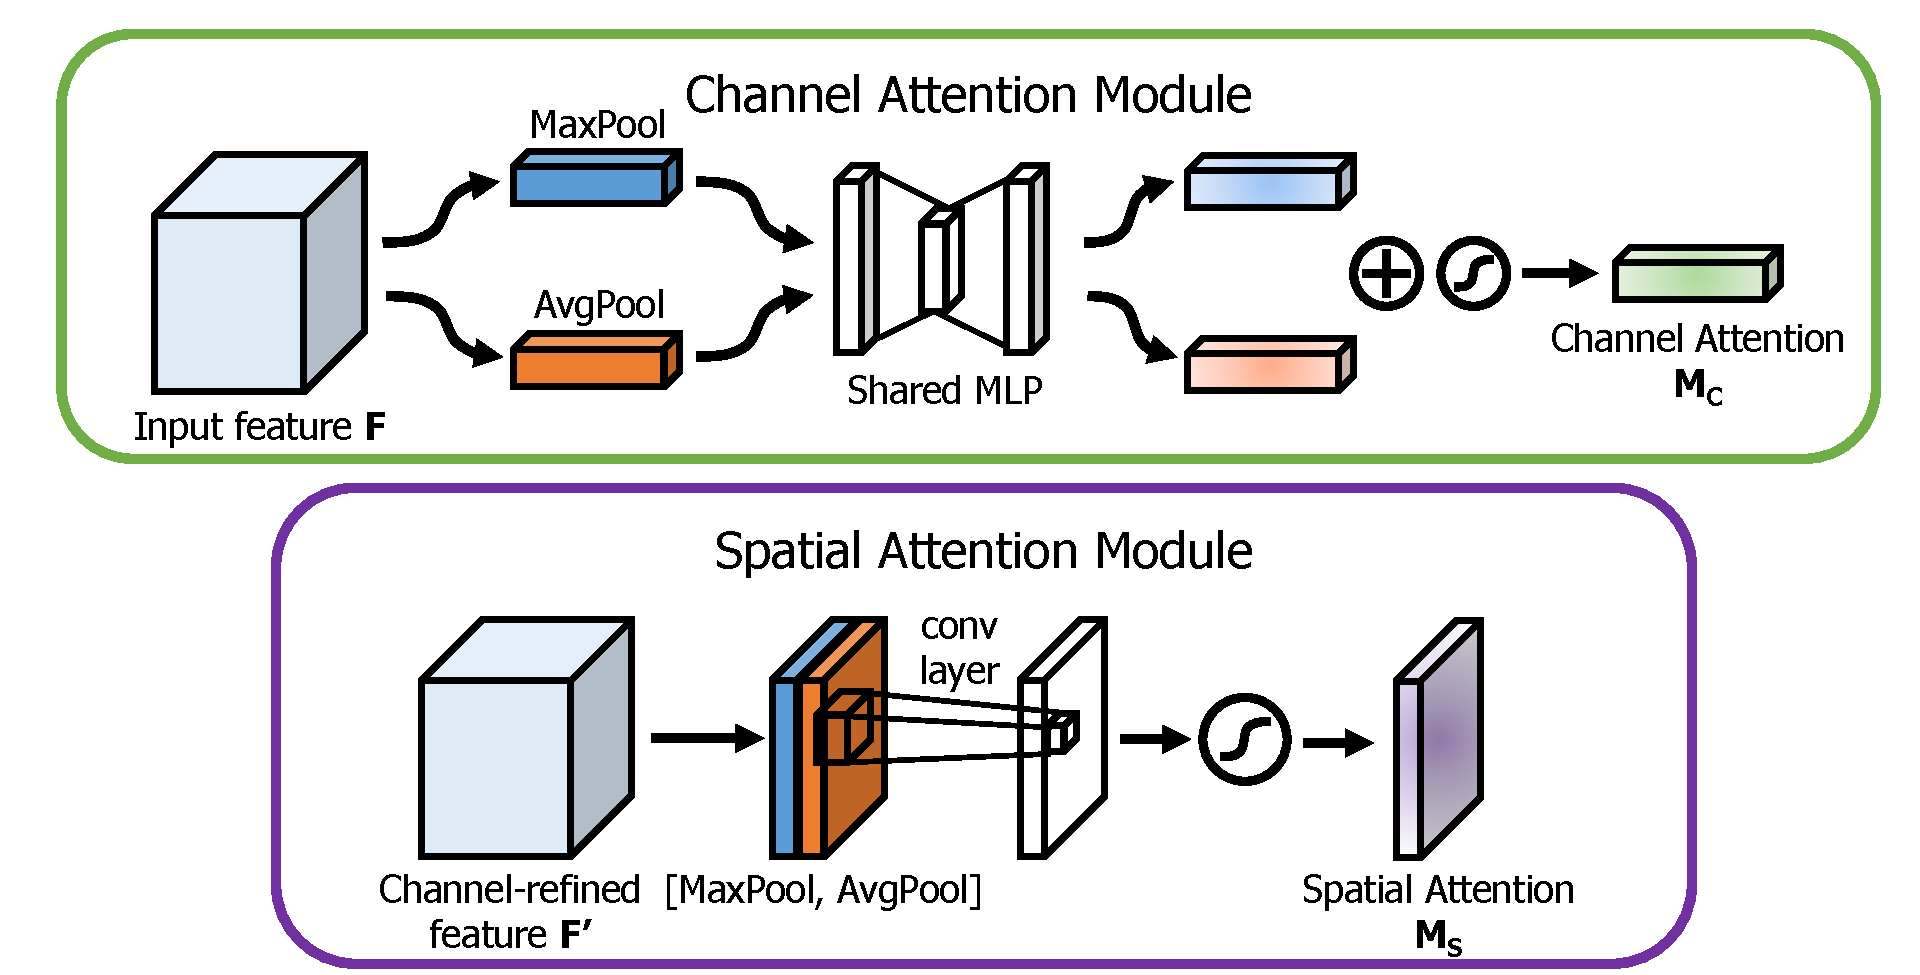
\includegraphics[width=\textwidth]{CBAM-Block.pdf}
  \caption{CBAM模块结构}
  \label{fig:CBAM-Block}
\end{figure}

scSE同样结合了通道注意力机制与空间注意力机制,基于SENet提出了一种通道注意力模块(Channel Squeeze-and-Excitation,cSE)和一种空间注意力模块(Spatial Squeeze-and-Excitation,sSE),其结构如图~\ref{fig:scSE}~所示,不同于CBAM,scSE的两个子模块并行处理原始输入,分别在空间维度和通道维度对原始输入进行加权,最后再进行特征图的融合。具体而言,cSE模块中,原始输入依次经过了空间维度的全局平均池化,通道维度的卷积降维与升维,以及非线性变换,以得到通道注意力权重。sSE模块中,直接通过深度卷积在通道维度进行降维,再经过非线性变换以得到空间注意力权重。
\begin{figure}
    \centering
    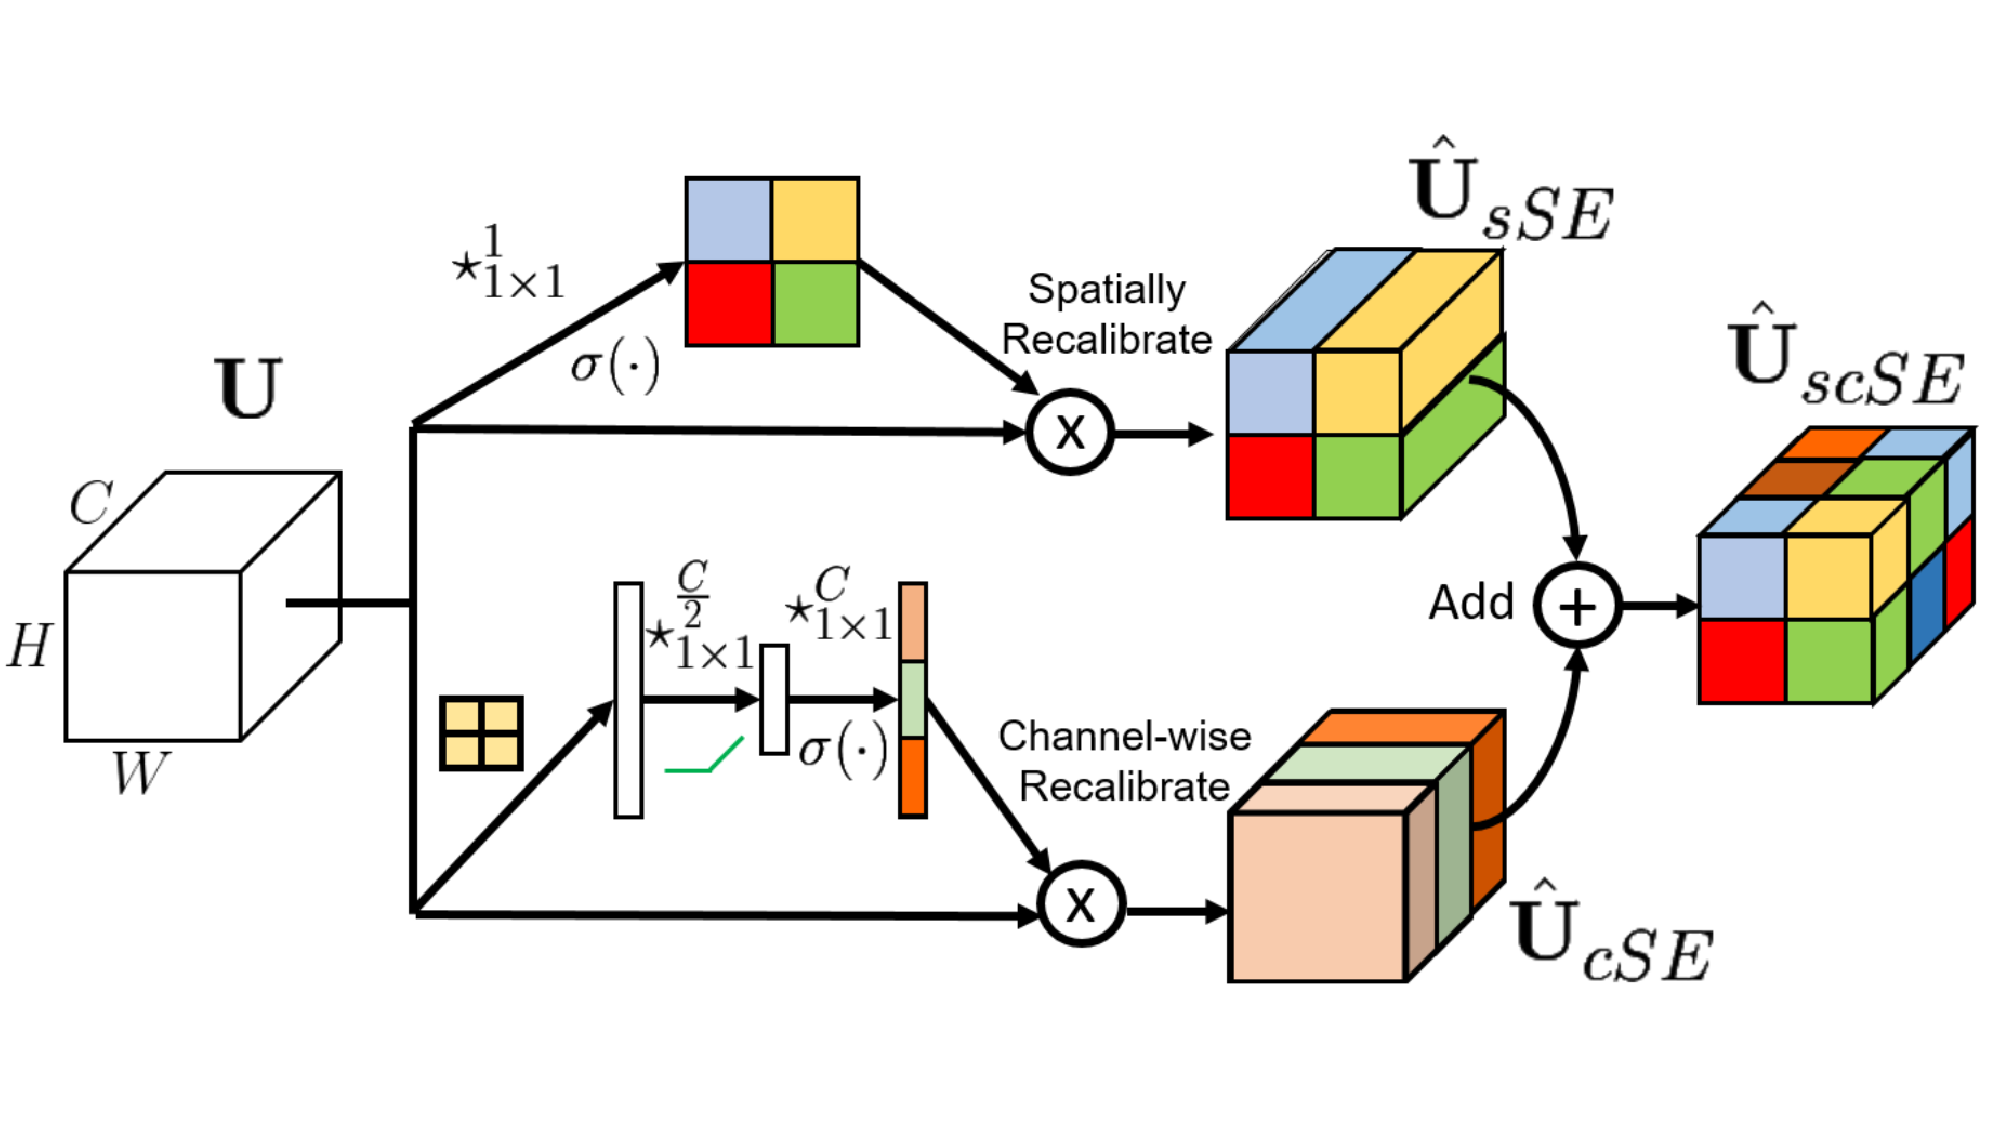
\includegraphics[width=\textwidth]{scSE.pdf}
    \caption{scSE结构}
    \label{fig:scSE}
\end{figure}

注意力机制通过动态分配权重,使得模型能够聚焦于输入数据中的关键信息,削弱噪声的影响,混合注意力机制则结合了多种注意力机制的优点,从而能够更全面地捕获和整合不同维度的数据特征,并在许多情况下展现出优于单一注意力机制的性能。因此,论文将升维处理后的EEG信号视作具有深度信息的图像数据,采用结合了深度注意力和空间注意力的混合注意力机制对BaseNet进行改进。

CBAM模块和scSE模块均为轻量级注意力模块,且均兼顾深度注意力和空间注意力,但scSE模块在参数数量上更具优势。与此同时,文献\cite{roy2018concurrent}研究发现scSE模块在语义分割任务上表现出色,特别是在与EEG信号拥有相似生理特性的医学图像的分割任务,其性能优于CBAM模块。基于以上理由,论文选择将scSE模块引入BaseNet模型中。由于BaseNet的特征提取过程分为时间卷积和空间卷积两个阶段,scSE模块可采取以下三种引入方式:其一是在时间卷积层后引入;其二是在空间卷积层后引入;其三是同时在时间卷积层和空间卷积层之后引入。图~\ref{fig:att-Base}~展示了这三种引入scSE模块的方式,从左至右分别是时间卷积层后引入scSE模块、空间卷积层后引入scSE模块,以及在时间卷积和空间卷积层后均引入scSE模块。将这三种引入方式对应的模型分别简称为S-Temporal-BaseNet、S-Spatial-BaseNet、S-TS-BaseNet。
\begin{figure}
  \centering
  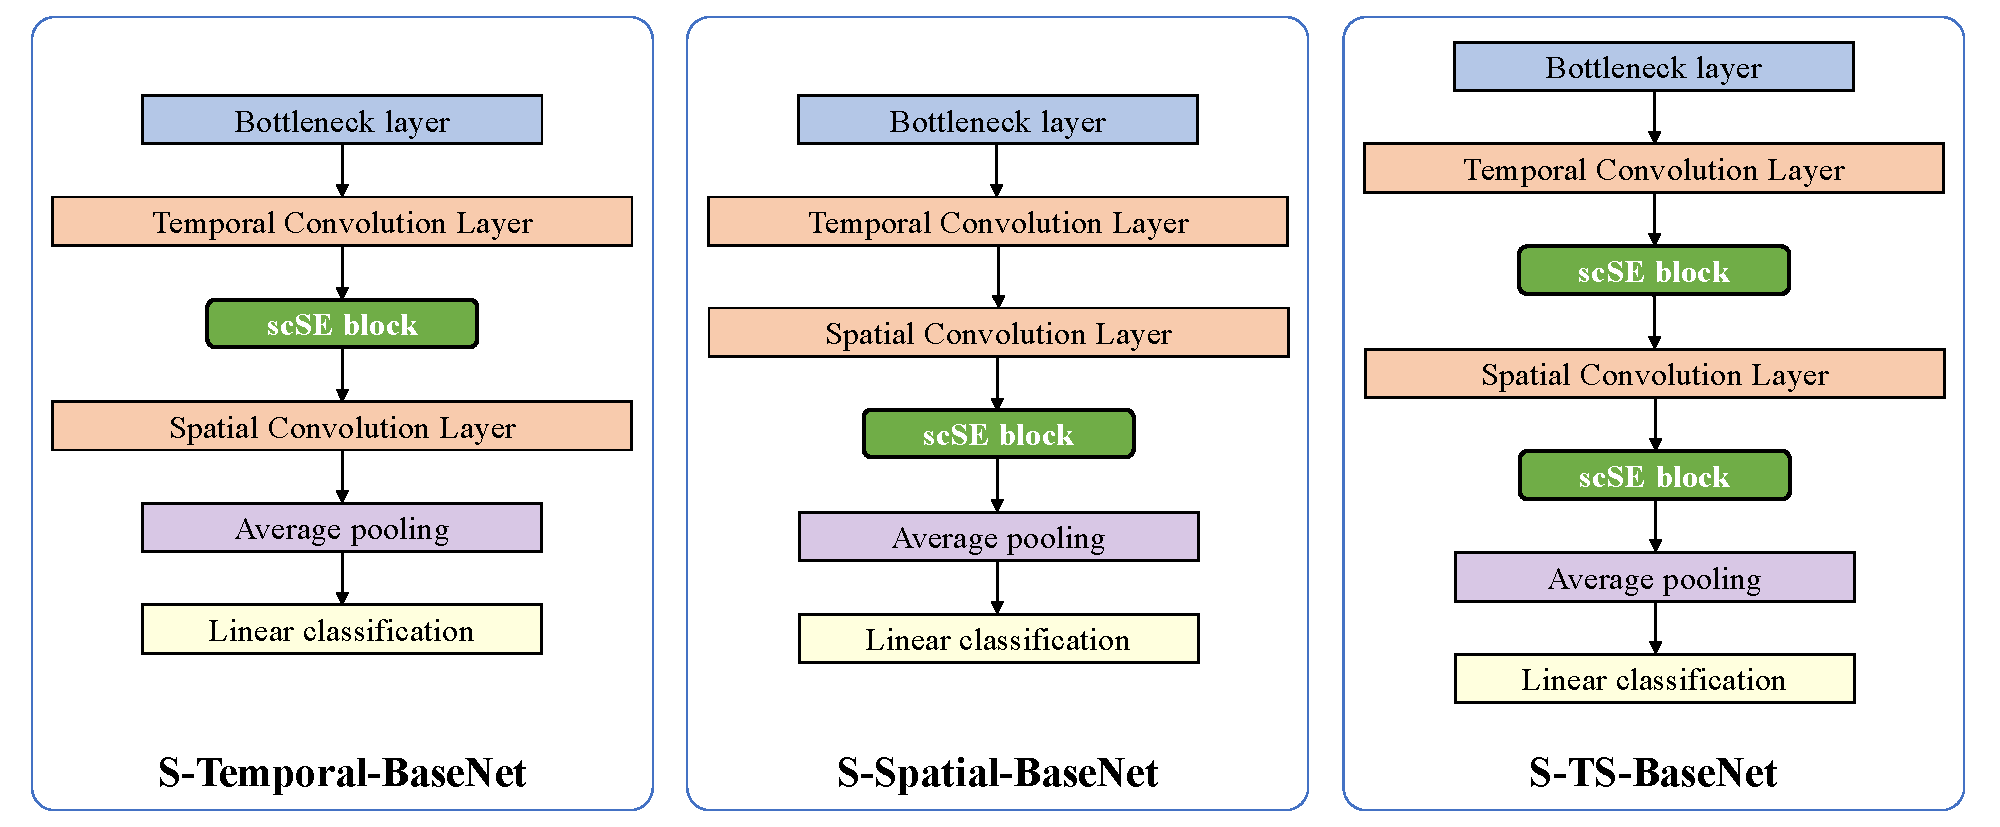
\includegraphics[width=\textwidth]{att-Base.pdf}
  \caption{BaseNet引入注意力模块的方式}
  \label{fig:att-Base}
\end{figure}

表~\ref{tab:scSE-BaseNet}~展示了S-Temporal-BaseNet、S-Spatial-BaseNet、S-TS-BaseNet三种模型在BCI Competition IV Dataset 2A\cite{tangermann2012review}数据集上的对比实验结果。实验采用固定的参数,表格中展示的准确率(Accuracy,ACC)和Kappa一致性系数(Kappa)指标为数据集中九位受试者的平均表现,标准差(Standard Deviation,SD)则为准确率的标准差。从准确率和一致性分析,S-ST-BaseNet模型的效果优于其他两种模型,与经验相符。此外,S-Temporal-BaseNet模型的效果优于S-Spatial-BaseNet模型,其原因可能在于,空间卷积层沿通道维度的卷积和沿深度维度的降维使得数据损失了部分特征,进而减弱了scSE模块提取关键特征权重的能力,而时间卷积层保留了大部分深度信息和通道信息,因此,在时间卷积层之后加入scSE模块能够帮助模型更好地捕捉深度和空间的特征。从标准差分析,S-TS-BaseNet模型的准确率波动幅度较小,对不同受试者的MI-EEG分类效果相对均衡,另外两种模型在不同受试者间的分类精度则存在较为明显的差异。实验数据显示,S-TS-BaseNet模型在增加了少量参数的情况下,取得了更好的效果,因此,论文采用同时在时间卷积层和空间卷积层之后引入scSE模块的方式,将这种结构的模型称为S-BaseNet。
\begin{table}[ht]
  \centering
  \caption{scSE模块引入位置对比}
  \label{tab:scSE-BaseNet}
  \begin{tabularx}{\textwidth}{CCCCC}
    \toprule
    \makebox[0.2\textwidth][c]{Models} & \makebox[0.2\textwidth][c]{ACC(\%)} & \makebox[0.2\textwidth][c]{Kappa} & \makebox[0.2\textwidth][c]{SD} & \makebox[0.2\textwidth][c]{Parameters} \\
    % Models & ACC(\%) & Kappa & SD & Parameters \\
    \midrule
    \makebox[0.2\textwidth][c]{S-Temporal-BaseNet} & \makebox[0.2\textwidth][c]{78.09} & \makebox[0.2\textwidth][c]{0.71} & \makebox[0.2\textwidth][c]{10.38} & \makebox[0.2\textwidth][c]{4702} \\
    \makebox[0.2\textwidth][c]{S-Spatial-BaseNet} & \makebox[0.2\textwidth][c]{77.16} & \makebox[0.2\textwidth][c]{0.69} & \makebox[0.2\textwidth][c]{10.24} & \makebox[0.2\textwidth][c]{\textbf{4357}} \\
    \makebox[0.2\textwidth][c]{S-TS-BaseNet} & \makebox[0.2\textwidth][c]{\textbf{78.55}} & \makebox[0.2\textwidth][c]{\textbf{0.71}} & \makebox[0.2\textwidth][c]{\textbf{9.46}} & \makebox[0.2\textwidth][c]{4765} \\
    \bottomrule
  \end{tabularx}
\end{table}

为取得更好的效果,对scSE模块进行改进。针对cSE模块,采用全局最大池化取代全局平均池化操作,实验证明了这一改动使模型具有更好的效果。此外,将scSE模块中的Sigmoid激活函数替换为Softmax激活函数,旨在更好地利用全局信息。针对sSE模块,论文提出两种方式进行改进,并将两种方式所得的权重相结合以获取最终的输出:

(1) 由CBAM模块的多维全局池化思想以及FBCNet模型的方差层设计\cite{mane2021fbcnet}得到启发,采用深度维度上的全局平均池化和全局方差计算操作代替原模块中的压缩操作,随后通过深度卷积对深度维度的特征图进行聚合,在更好地表征EEG信号特性的同时,进一步降低了参数规模;

(2) 考虑EEG信号中的时空权重无关性,即空间特征权重代表电极重要程度,时间特征权重代表采样点重要程度,分两个维度提取特征。对于空间维度,首先进行深度压缩操作,随后通过时间维度上的平均池化和最大池化得到两个特征图,通过1\times1卷积对这两个特征图进行融合。对于时间维度,进行空间维度上的卷积操作,以得到时序权重。最后,将空间权重与时序权重相乘,恢复维度。

得到论文将改良后的scSE模块称为svSE(Separate Variance-Informed Spatial and Channel Squeeze-and-Excitation)模块,其结构如图~\ref{fig:svSE}~所示。使用svSE模块替换S-BaseNet模型中的scSE模块。
\begin{figure}
  \centering
  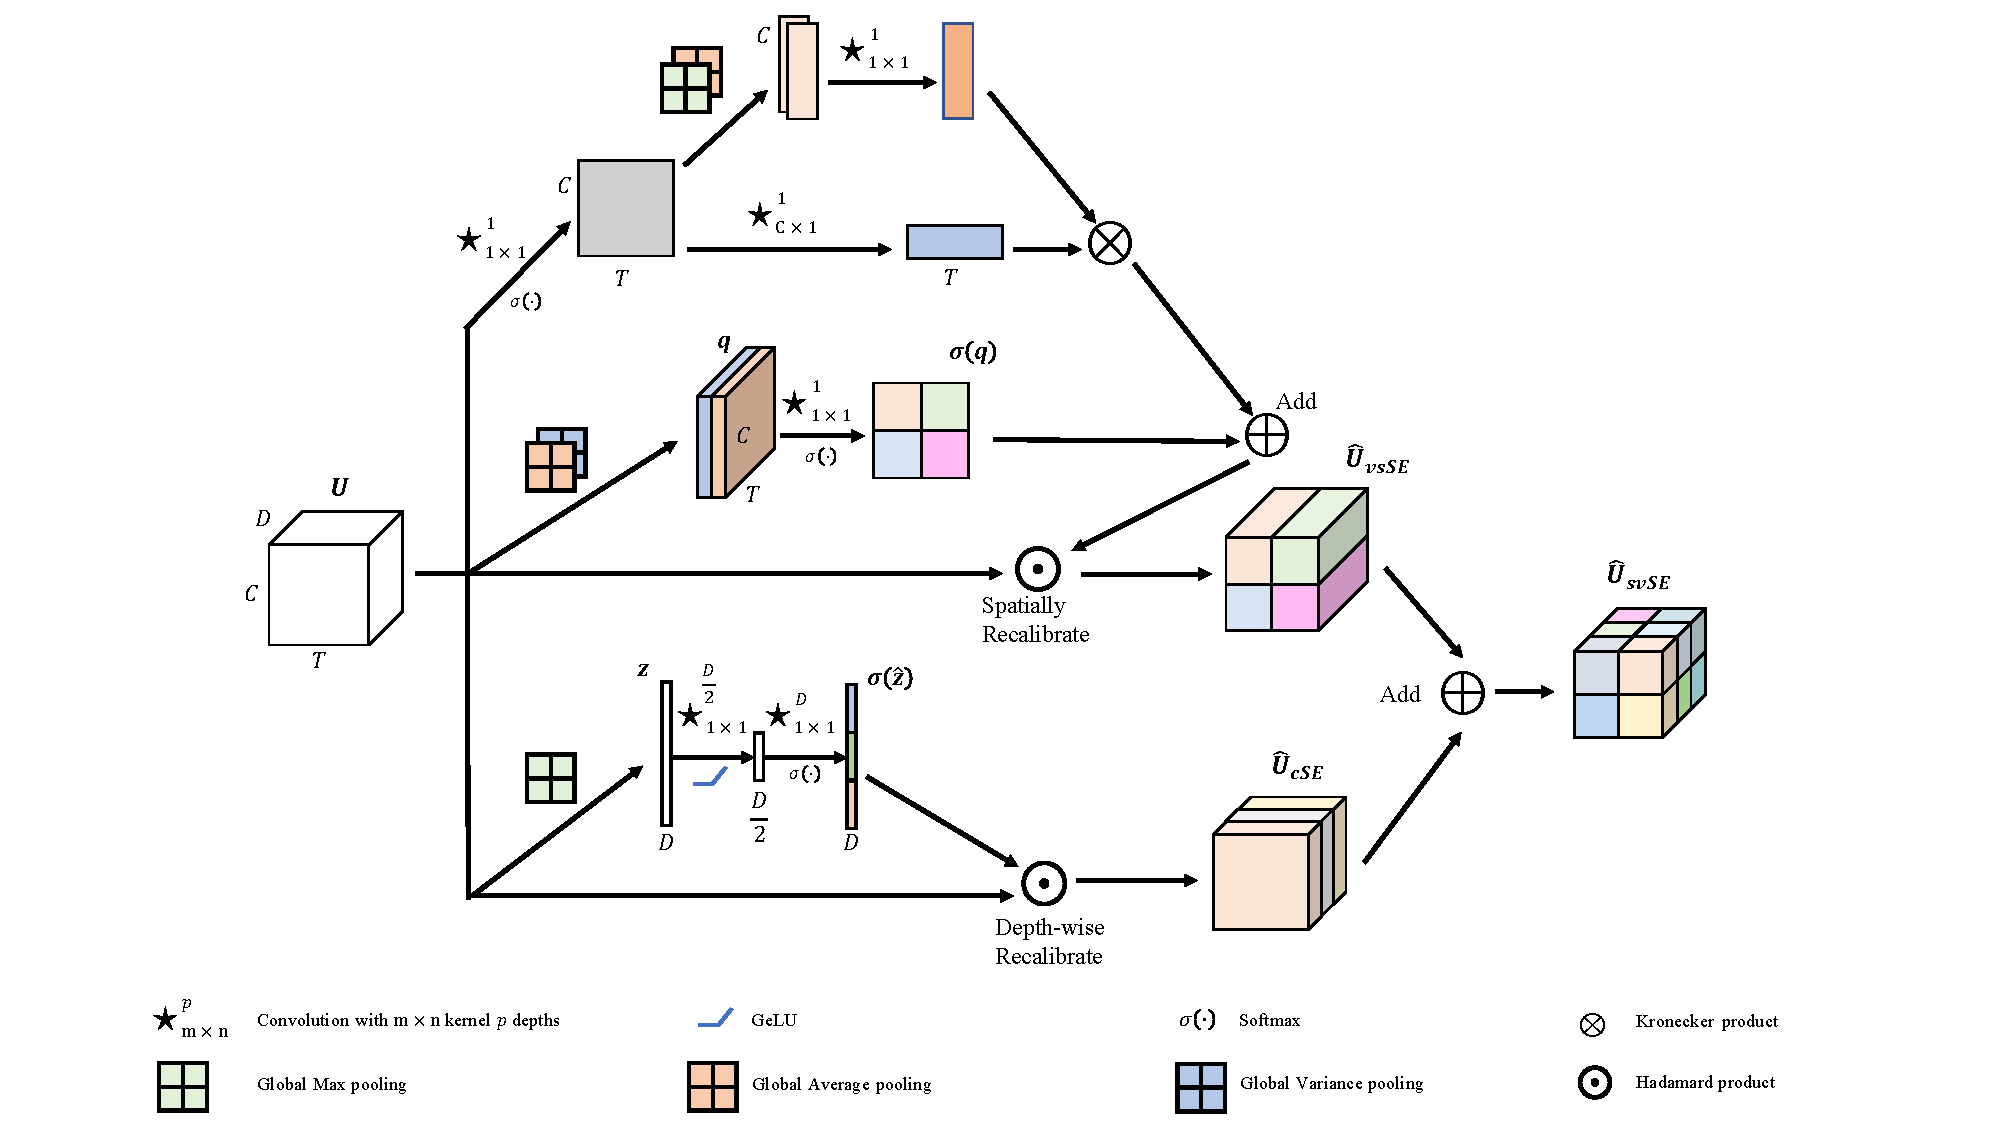
\includegraphics[width=\textwidth]{svSE.pdf}
  \caption{svSE结构}
  \label{fig:svSE}
\end{figure}

\subsection{基于密集连接优化Inception模块}

在构建BaseNet时,论文发现U-Net在处理MI-EEG分类任务时同样展现了一定的优势。由于EEG信号的特征相对简单,因此低级特征与高级语义信息都相对重要,U-Net因其特殊的跳跃连接结构有效地融合了这两种信息,然而,U-Net中通过解码器阶段将特征图恢复至原始空间尺寸的操作并非必要,因为在分类任务中,这种重建过程可能导致额外的计算负担且对分类性能的提升效果不明显。因此,在对VSNet进行改进时,论文从U-Net兼顾低级特征与高级语义信息的策略中得到启发,同时对不必要的特征图空间尺寸还原过程进行规避,以构建一个既能充分利用EEG信号中各级别特征信息,又具备高效计算能力的改进模型。

Gao Huang等人于2016年提出了密集连接网络\cite{huang2017densely}(Dense Convolutional Network,DenseNet)。在ResNet的基础上,DenseNet提出了一种更为激进的连接模式:引入从任意层到后续层的直接连接,即密集连接(Dense Connection)。DenseNet的第 \(l\) 层接收所有前序特征图为输入,其输出为 \(x_l\):
\begin{equation}
  x_l = H_l([x_0, x_1, ···, x_{l-1}])
  \label{eq:dense-conn}
\end{equation}
其中,\([x_0, x_1, ···, x_{l-1}]\) 代表第 \(0, ···, l-1\) 层的输出特征图,\(H_l(·)\) 代表非线性转换复合函数,可能包括一系列的批量归一化、ReLU、池化及卷积操作。密集连接的结构如图~\ref{fig:denseBlock}~所示。
\begin{figure}
  \centering
  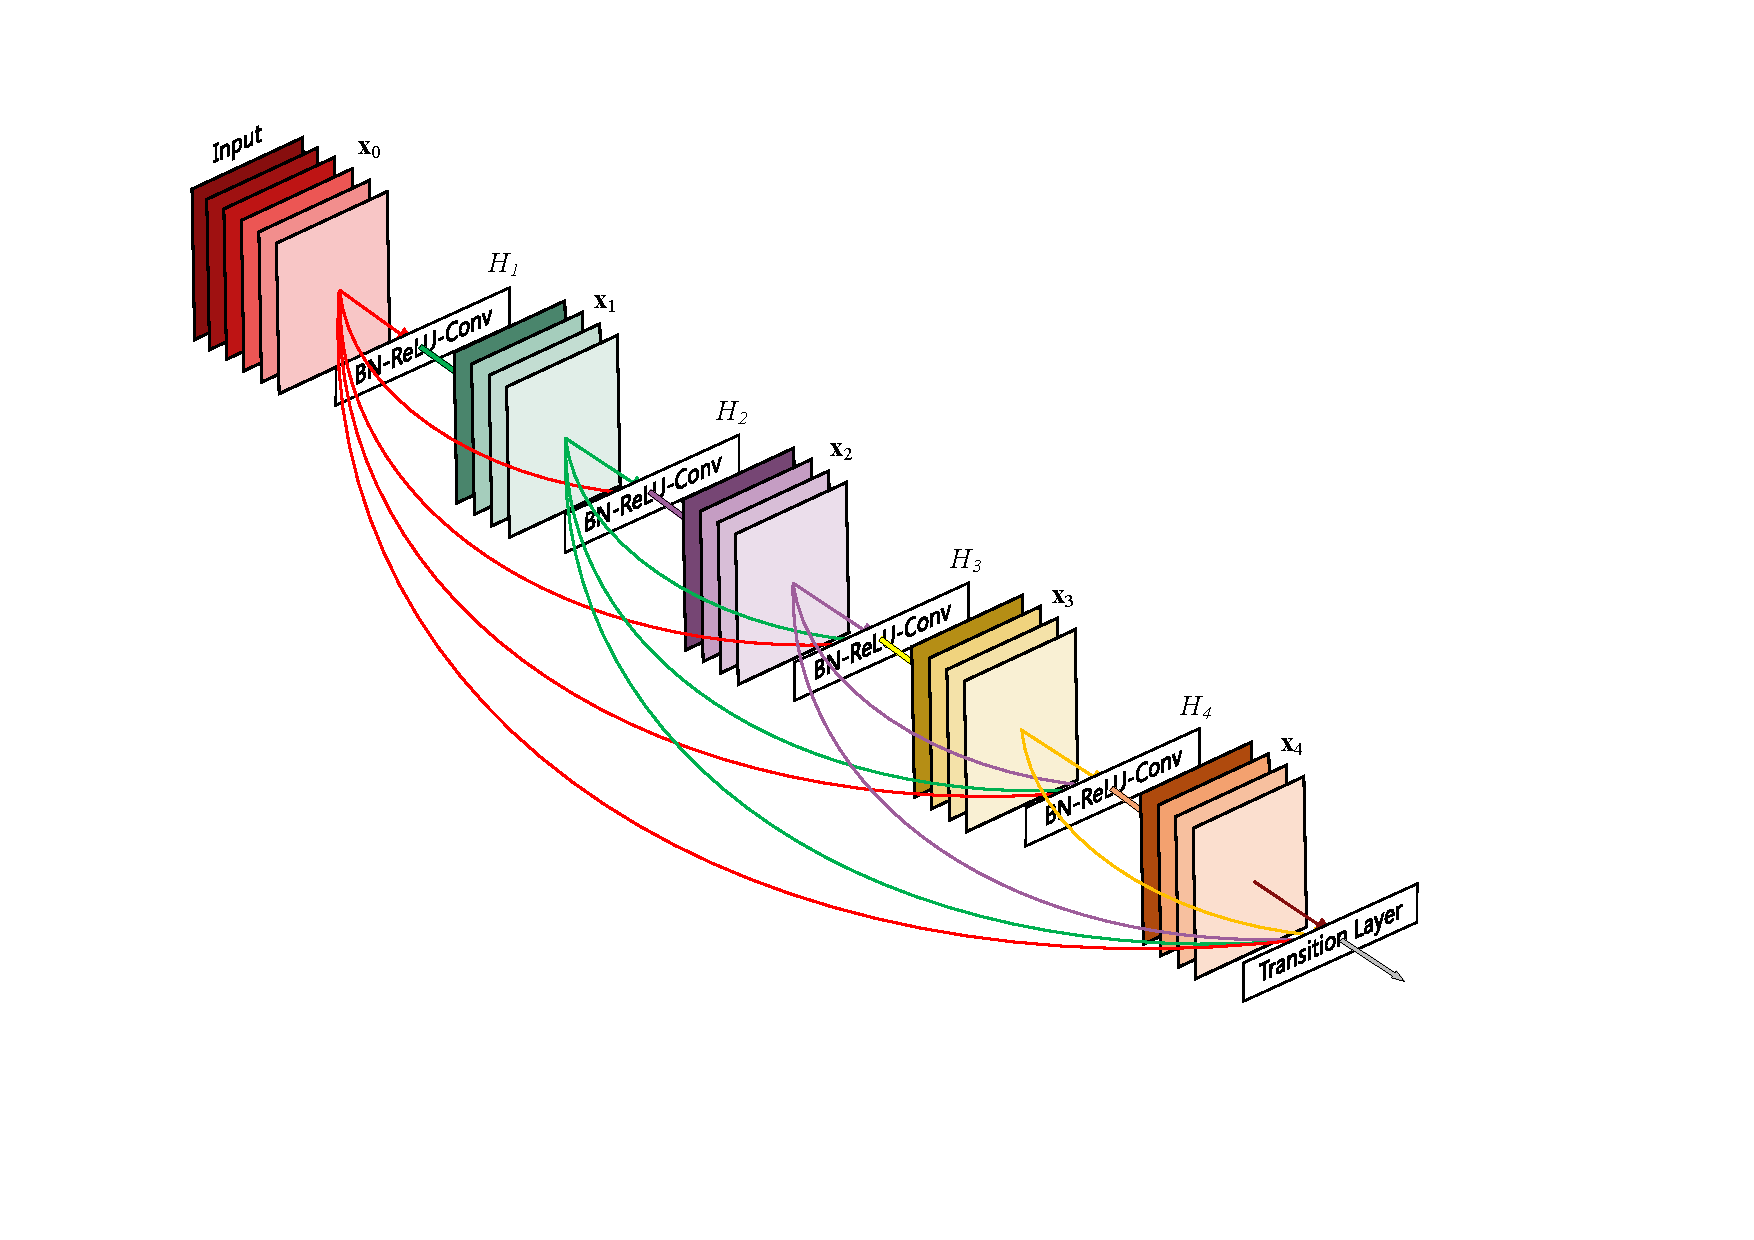
\includegraphics[width=0.8\textwidth]{denseBlock.pdf}
  \caption{密集连接结构}
  \label{fig:denseBlock}
\end{figure}

在密集连接模块中,所有的前序特征图通过Concentrate在深度维度上连接在一起,因此,在一个密集连接模块中所有特征图的大小是相同的。DenseNet提出了Transition模块用于连接两个相邻的密集连接模块,并通过池化操作对特征图进行下采样,从而减小特征图的大小。

通过密集连接的方式,网络中的每一层都能够访问并整合所有前序层提取出的特征信息,进而充分利用EEG信号中的低层特征细节和高层语义信息。相较于U-Net中的编码-解码结构,密集连接无需经历数据空间的重建过程,即可实现特征的有效复用。此外,DenseNet中的Transition模块也为实现特征图的下采样提供了思路。

在DenseNet中,有两种不同构造的密集连接模块,分别是基础密集连接模块(Basic Dense Block)和带有瓶颈层的密集连接模块(Bottleneck Dense Block),它们的区别主要体现在非线性转换复合函数 \(H(·)\) 的设计上:

(1) 基础密集连接模块(Basic Dense Block):其非线性转换复合函数定义为: \(H(·) = BN + ReLU + 3 \times 3\;conv\)。

(2) 瓶颈密集连接模块(Bottleneck Dense Block):其非线性转换复合函数更为复杂,包括两个卷积层、两次BN和ReLU激活:\(H(·) = BN + ReLU + 1\times1\;conv + BN + ReLU + 3 \times 3\;conv\)。加入瓶颈层的主要原因在于降低特征维度的数量,从而提升模型计算效率。

为了同时利用Inception模块多尺度并行特征提取和密集连接兼顾深层与浅层特征的优点,论文选择将Bottleneck Dense Block嵌入Inception模块中,替代原本的时间卷积核。为了简洁起见,下文称之为密集连接模块。

原始的密集连接模块在计算机视觉图像分类任务中都取得了优秀的表现,在设计上,它考虑到了图像数据在空间维度具有等价的重要性。然而,EEG信号的时空信息具有不均衡的重要性,通常情况下,时间维度往往比空间维度蕴含更为丰富的信息。与此同时,研究指出\cite{lawhern2018eegnet},当设计用于提取EEG特征的卷积核时,将时间卷积核长度设置为EEG信号采样率的一半,可以有效地捕获2Hz及以上频段的信号信息。因此,在处理EEG信号时,时间卷积核的长度应当依据EEG信号的实际采样率来灵活设定,以便提取不同频率成分的信号特征。

鉴于上述EEG信号与图像数据的特性差异,对原始密集连接模块的卷积核进行改造。将密集连接模块中的卷积核概念转化为针对时间序列的一维卷积(尽管在实现时仍采用二维卷积),为了更好地匹配EEG信号的采样特性及其内在频率成分,依据EEG信号的采样频率 \(sfreq\) 来动态调整位于Inception第 \(i\) 个分支上的密集连接模块的时间卷积核大小 \(kernel_i\),具体公式如下:
\begin{equation}
    kernel_i = sfreq \times time\_unit_i, \quad time\_unit_i \in \{0.1, 0.3, ···, 0.9\}
    \label{eq:kernel_cal}
\end{equation}
其中,\(sfreq\) 是EEG信号的采样频率,\(time\_unit_i\)  则为卷积核对应的时间单位,其取值范围分布在0.1秒至0.9秒的奇数间隔内。这样设置卷积核大小是为了更全面地捕捉EEG信号中不同频率成分的特征信息,同时避免因卷积核大小过于接近而导致提取的特征之间重叠度过高。例如,当采样周期设定为0.5秒时,卷积核大小将是采样率的一半,进而能够有效地捕获到2Hz及更高频段的EEG信号特征。

由此,密集连接模块的非线性转换复合函数 \(H(·)\) 定义如下:
\begin{equation}\label{eq:dense-kernel}
    \begin{split}
      &H(·) = BN + GeLU + 1\times1\;conv + BN +  1 \times kernel_i\;conv + Dropout \\
      &kernel_i = sfreq \times time\_unit_i, \quad time\_unit_i \in \{0.1, 0.3, ···, 0.9\}
    \end{split}
\end{equation}
相较于原始模块,论文在前文研究的基础上做出了以下改进,分别为:根据EEG信号的特性调整了卷积核大小;选用性能更优的激活函数GeLU替代ReLU;引入了Dropout层,以进一步缓解过拟合现象。

经过以上改进,新构建模型的结构如图~\ref{fig:incep-dense}~所示,将其命名为DIS-Net。Dense-Inception module构成了时间卷积层,其内部的各个分支均由一系列改进版的Bottleneck Dense Block紧密堆叠而成,形成密集连接结构,用以同时获取浅层和深层的时间特征。每个分支提取的特征图在深度维度上进行聚合,并通过Transition模块进行深度压缩和特征整合,以进一步提升模型的表达能力和计算效率。需要说明的是,Dense-Inception module的数量,以及Dense-Inception module的分支数量、Dense block的数量,都是可调的超参数。
\begin{figure}
  \centering
  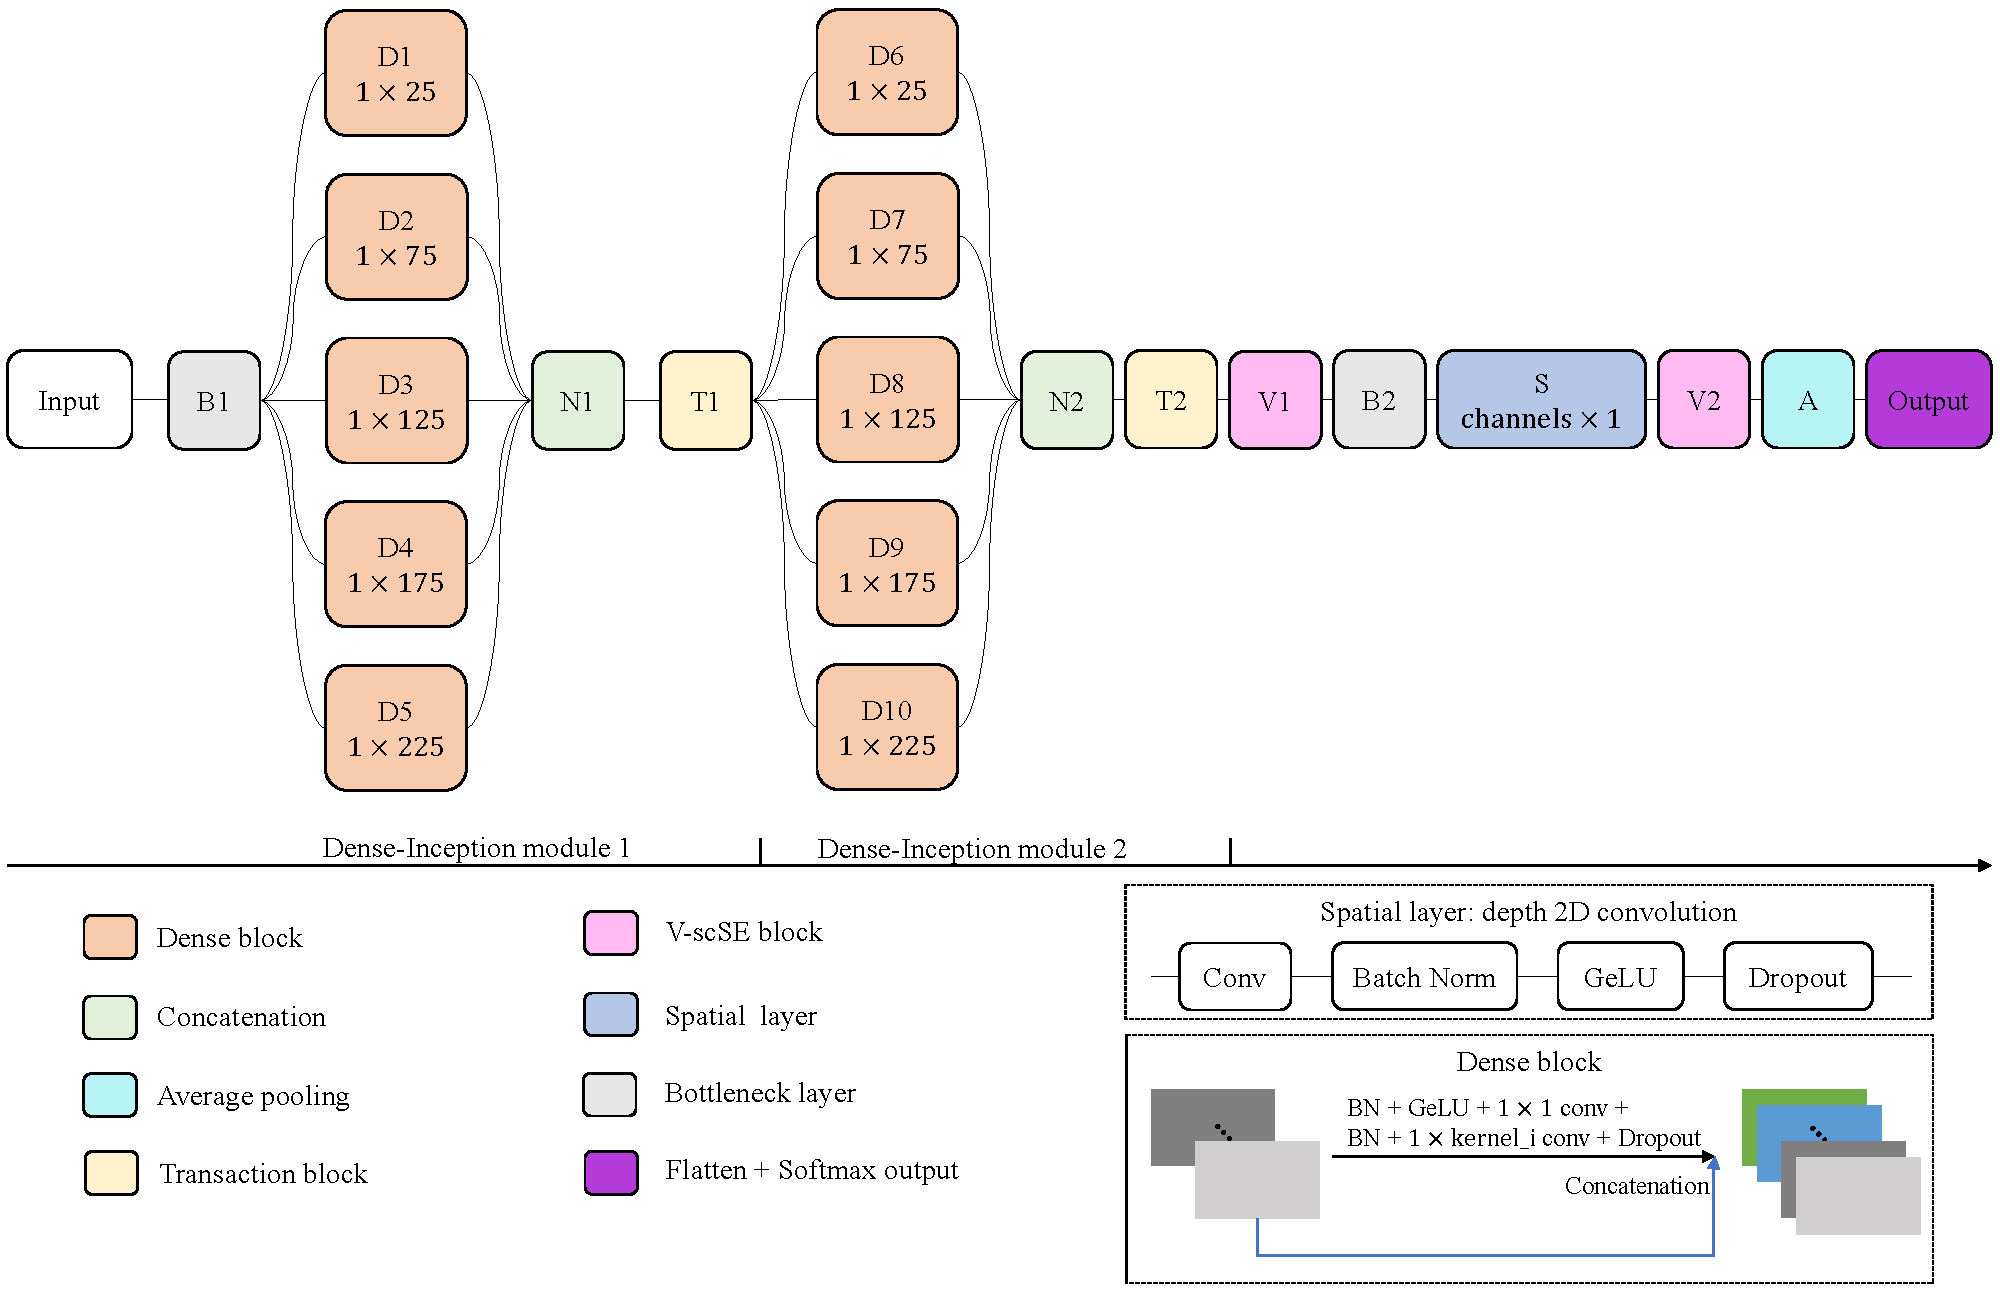
\includegraphics[width=\textwidth]{incep-dense.pdf}
  \caption{DI-VSNet结构}
  \label{fig:incep-dense}
\end{figure}

\subsection{基于Transformer构建并行分支}

卷积神经网络中,尽管卷积层因其局部感受野能够出色地捕获信号中的局部时空特征,但对于那些跨越较长时间跨度和空间分布的复杂交互信息,其建模能力受限。而Transformer模型\cite{vaswani2017attention}因其自注意力机制(Self-Attention)可以在不考虑输入位置顺序的情况下,灵活地捕捉并编码任意两点之间的相互依赖关系,从而能够更有效地理解和处理长距离依赖,但与此同时,其可能无法充分提取局部时空特征。因此,论文选择将两者进行结合,用于MI-EEG分类任务。

原始的Transformer模型是编码器-解码器(Encoder-Decoder)结构,编码器模块负责接收输入序列,并通过自注意力机制捕捉并整合整个序列中的语义和上下文信息;解码器则依据这些编码后的信息逐步生成对应的输出序列。在MI-EEG分类任务中,不涉及目标序列的生成,因此只需要使用Transformer的编码器,其结构如图~\ref{fig:encoder}~所示。
\begin{figure}
    \centering
    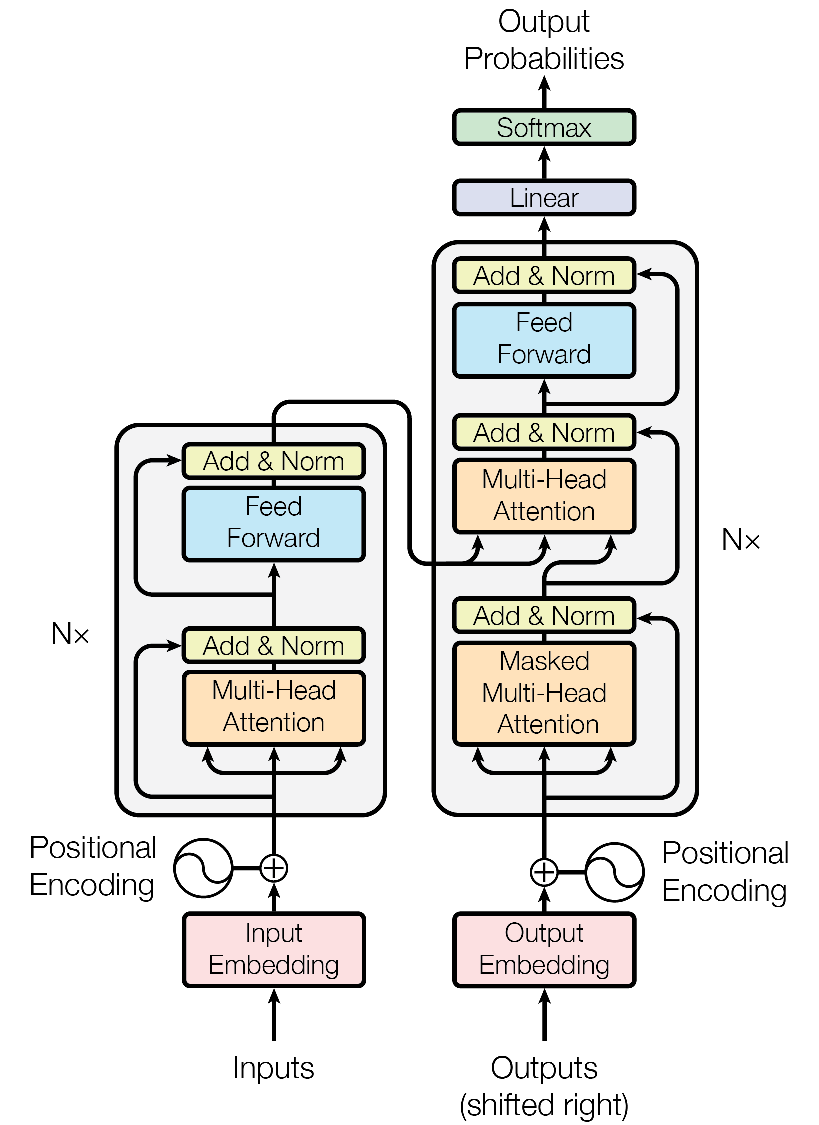
\includegraphics[height=0.7\textwidth]{encoder.pdf}
    \caption{Transformer Encoder结构}
    \label{fig:encoder}
\end{figure}
编码器由以下几部分组成:

(1) 输入嵌入与位置编码层(Input Embedding \& Positional Encoding):将输入序列转化为稠密向量表示,通过位置编码为输入添加位置信息。

(2) 多头注意力(Multi-Head Attention):使用多个并行运行的自注意力(Self-Attention)子层(头),提取不同尺度的长距离依赖,对输入进行注意力加权。

(3) 残差连接与层归一化(Add \& Norm):在每个子层之后应用残差连接与层归一化,提高模型训练效率和稳定性,避免网络退化。

(4) 前馈神经网络(Feed Forward):全连接神经网络,对多头注意力的输出进行非线性转换。

对于MI-EEG信号而言,空间维度的特征反映了电极位置特异性,时间维度的特征则体现了与事件相关去同步(ERD)和事件相关同步(ERS)等生理现象相关的时序变化。因此,重要的长依赖关系主要存在于在时间维度,即时序特征。因此,论文使用的Transformer模块沿袭经典Transformer结构。

为了更好地获取时序长依赖,将一个输入样本 \(X \in \mathbb{R}^{C \times T}\) 中的第 \(i\) 个时间序列视为一个Token \(x_i \in \mathbb{R}^{T}\),则一个样本需要 \(C\) 个Transformer处理,表达为:
\begin{equation}\label{eq:multi-trans}
    f(X)={\textstyle \sum_{i}^{C}}f_i(x_i)
\end{equation}。
其中,\(C\) 代表数据的通道数, \(T\) 代表时间序列长度。考虑单个Transformer,获得其对应的 \(x\) 的词嵌入表示 \(E \in \mathbb{R}^{T \times d_model}\) ,其中,\(d_model\) 为词嵌入维度,随后对Token \(E\) 的处理过程如下:

首先,为了编码序列的位置信息,论文对 \(E\) 进行可学习位置编码,即通过一个可学习的参数矩阵表征Token的位置信息,将其记为\(PE\),通过相加的方式与Token相融合,获得最终的Token \,\(Y\): \(Y=E+PE\)。

随后,对于 \(Y\),通过含多个自注意力机制的多头注意力层(MHA)进行处理。对于第 \(i\) 个头(head),首先通过三组线性变换,获得Query \(Q_i\),Key \(K_i\),Value \(V_i\),如公式~\ref{eq:change}所示:
\begin{equation}\label{eq:change}
    Q=W^{Q}_iY,\,K=W^{K}_iY,\,V=W^{V}_iY
\end{equation}
其中,\(W^{Q}_i,\,W^{K}_i,\,W^{V}_i \in \mathbb{R}^{d_model \times d_k}\),\(d_k=d_model \div h\),\(h\)是head的数量。通过公式~\ref{eq:sa}~得到当前head的输出,记为\(A_i\):
\begin{equation}\label{eq:sa}
    A_i=softmax(\frac{Q_iK^{T}_i}{\sqrt{d_k}}V_i)
\end{equation}
随后,根据公式~\ref{eq:mha}~对所有head的结果进行合并:
\begin{equation}\label{eq:mha}
    MHA(Y)=Concat(A_1,...,A_h)W^{O}
\end{equation}
其中,\(W^{O} \in \mathbb{R}^{T \times d_model}\),输出经过残差连接和层归一化:
\begin{equation}\label{eq:rl}
    Z=LayerNorm(Y+MHA(Y))
\end{equation}

MHA的输出会在全连接前馈神经网络(FFN)中进行转换,并同样经过残差连接和层归一化,由公式~\ref{eq:ffn}得到最终的输出。
\begin{equation}\label{eq:ffn}
    \hat{Z}=LayerNorm(Z+FFN(Z))
\end{equation}

论文从深度残差收缩网络(Deep Residual Shrinkage Network,DRSN)\cite{zhao2019deep}中得到启发,对于具有低信噪比的EEG数据,将软阈值函数(Soft Thresholding)引入Transformer中。软阈值函数是信号处理中常用的去噪方式\cite{wright2009sparse},其公式如下:
\begin{equation}\label{eq:soft}
    y=\left\{
    \begin{aligned}
    & x-\tau, \; x>\tau \\
    & \quad0, \quad -\tau \le x \le \tau \\ 
    & x+\tau, \; x<-\tau
\end{aligned}
\right.
\end{equation}
其中,\(x\) 为输入,\(y\) 为输出,\(\tau\) 为阈值。
软阈值函数将绝对值小于阈值的输入转为零值,同时对绝对值接近阈值的输入有抑制作用,从而能够减少噪声对特征的影响。论文在Transformer模块之后添加软阈值函数,通过公式~\ref{eq:tau}~计算阈值 \(\tau\):
\begin{equation}\label{eq:tau}
    \tau=\alpha \times Average(\hat{Z}),\quad \alpha \in (0,\,1)
\end{equation}
其中,\(\alpha\) 是一个可供学习的参数。通过这种方式,
\(\tau\) 是一个不太大的正数,从而避免输出全部为零的情况。

不同于Song等人将Transformer嵌入卷积神经网络之后的方式\cite{song2022eeg},论文选择以并行分支的形式引入Transformer模块。这是因为直接在卷积层之后加入Transformer可能导致模型仅能捕捉到深层卷积特征图的依赖关系,而非充分利用全局信息。并行分支的设计旨在全面利用Transformer对全局依赖的建模能力,同时避免干扰卷积神经网络本身的局部特征提取功能。

将Transformer模块引入DIS-Net后获得的新模型命名为HIT-Net,其结构如图~\ref{fig:HIT}~所示。为了综合CNN和Transformer提取的特征信息,将二者获取的特征图在深度维度进行特征聚合,因此,有必要对数据进行一定的处理,使得两个分支的数据形状相匹配。论文设计了CT-Block和TC-Block用于并行分支数据的交互融合。在CT-Block中,数据通过时间维度的池化和通道维度的卷积进行下采样,将一个样本 \(X \in \mathbb{R}^{C \times T}\) 沿通道维度压缩至 \(X^{'} \in \mathbb{R}^{C^{'} \times T}\) ,其中, \(C\) 代表通道数(电极数), \(T\) 代表时间序列长度,\(C^{'}\) 是一个大于等于1且小于等于 \(C\) 的整数,通常设定为 \(\left\lfloor \frac{C}{N} \right\rfloor\),\(N\) 为输出类别数量,这样设计的目的是减少计算开销和保留一定的空间特征信息。在TC-Block中,则通过反卷积对Transformer模块的输出进行重建,将时间维度和通道维度上采样至与CNN分支相同的大小。

\section{基于HIT-Net轻量化的端到端MI-EEG分类网络HIT-lightNet}

考虑到BCI系统对即时响应具有较高的要求,虽然HIT-Net已运用了瓶颈层、深度可分离卷积等手段有效地缩减了模型参数量,但为了追求更加卓越的实时性能表现,仍有进行进一步轻量化的必要。HIT-Net模型参数的主要来源在于Transformer模块和密集连接模块。针对Transformer模块的轻量化策略包括但不限于减少原始层级数目、量化参数类型及运用知识蒸馏技术。然而,面对小样本规模的EEG信号数据集,由于缺乏足够的大数据训练支撑,论文主要采取了减少原始层数这一轻量化途径。具体来说,对于CT-Block设计了更为高效的下采样方案,将原本由多个Transformer单元组成的Transformer分支精简为仅包含一个Transformer单元。与此同时,对于密集连接模块以及其他卷积层,论文进行针对性的轻量化卷积设计,并将在下文中对轻量化卷积模块的设计思路与方案加以阐述。

\subsection{经典轻量级网络结构}

MobileNet\cite{howard2017mobilenets}由Google团队提出,其核心思想在于引入了深度可分离卷积(Depthwise Separable Convolution),通过深度卷积处理单个输入通道,然后使用点积卷积(也称为逐点卷积或1x1卷积)跨通道整合信息。这种分解大幅减少了计算成本和模型大小,同时保持了较高的精度。在V2版本中,引入了反转残差(Inverted Residual)结构\cite{sandler2018mobilenetv2},不同于常规残差块的设计,它在网络较窄的地方采用线性瓶颈层增加深度,而非在宽度较大的地方。此外,MobileNetV2取消了线性瓶颈层后的小维度特征上的ReLU激活函数,以此来保持更多的非线性表达能力。V3版本在前两代的基础上,通过结合人类专家指导的网络设计原则与自动化的网络结构搜索(Network Architecture Search,NAS)技术\cite{howard2019searching},进一步定制了模型结构,即每个卷积层的具体通道数和操作类型都根据NAS的结果确定。此外,MobileNetV3还引入了Hard Swish这一新的激活函数以及其他的优化策略。

ShuffleNet\cite{zhang2018shufflenet}由旷视科技的研究团队所开发,其设计目标在于实现模型计算效率与预测准确性的均衡优化。为了解决分组卷积可能导致的组间特征孤立问题,ShuffleNet引入了通道混洗(Channel Shuffle)技术,即在执行完分组卷积之后,对各组内的特征图进行有序重组,以促进不同组间的特征信息相互交织和传播,从而增强模型的特征表达能力。此外,ShuffleNet针对分组卷积的配置进行了精细化调整,科学地配置组的数量和各组内的通道数,以便在有限的计算资源条件下最大限度地提升模型性能。在V2\cite{ma2018shufflenet}版本中,研究团队提出了一套高效卷积神经网络设计原则,并据此对ShuffleNetV1架构做出了改进。他们摒弃了1 \times 1的分组卷积操作,转而采用通用卷积来替代,并提出了通道分割(Channel Split)策略。具体而言,模型将输入特征图均匀划分为两个部分,一部分不经额外计算直接向下传输,另一部分则经历一系列计算后再与前者合并。在concatenate操作之后,继续实施通道混洗操作,从而有效提升模型在轻量化条件下的性能表现。ShuffleNet的结构如图~\ref{fig:shufflenet}~所示,图~\ref{fig:shufflenet}~(a)是ShuffleNet的基本单元,图~\ref{fig:shufflenet}~(b)在ShuffleNet基本单元的基础上增加了下采样,图~\ref{fig:shufflenet}~(c)是ShuffleNetV2的基本单元,图~\ref{fig:shufflenet}~(d)在ShuffleNetV2基本单元的基础上增加了下采样。
\begin{figure}
    \centering
    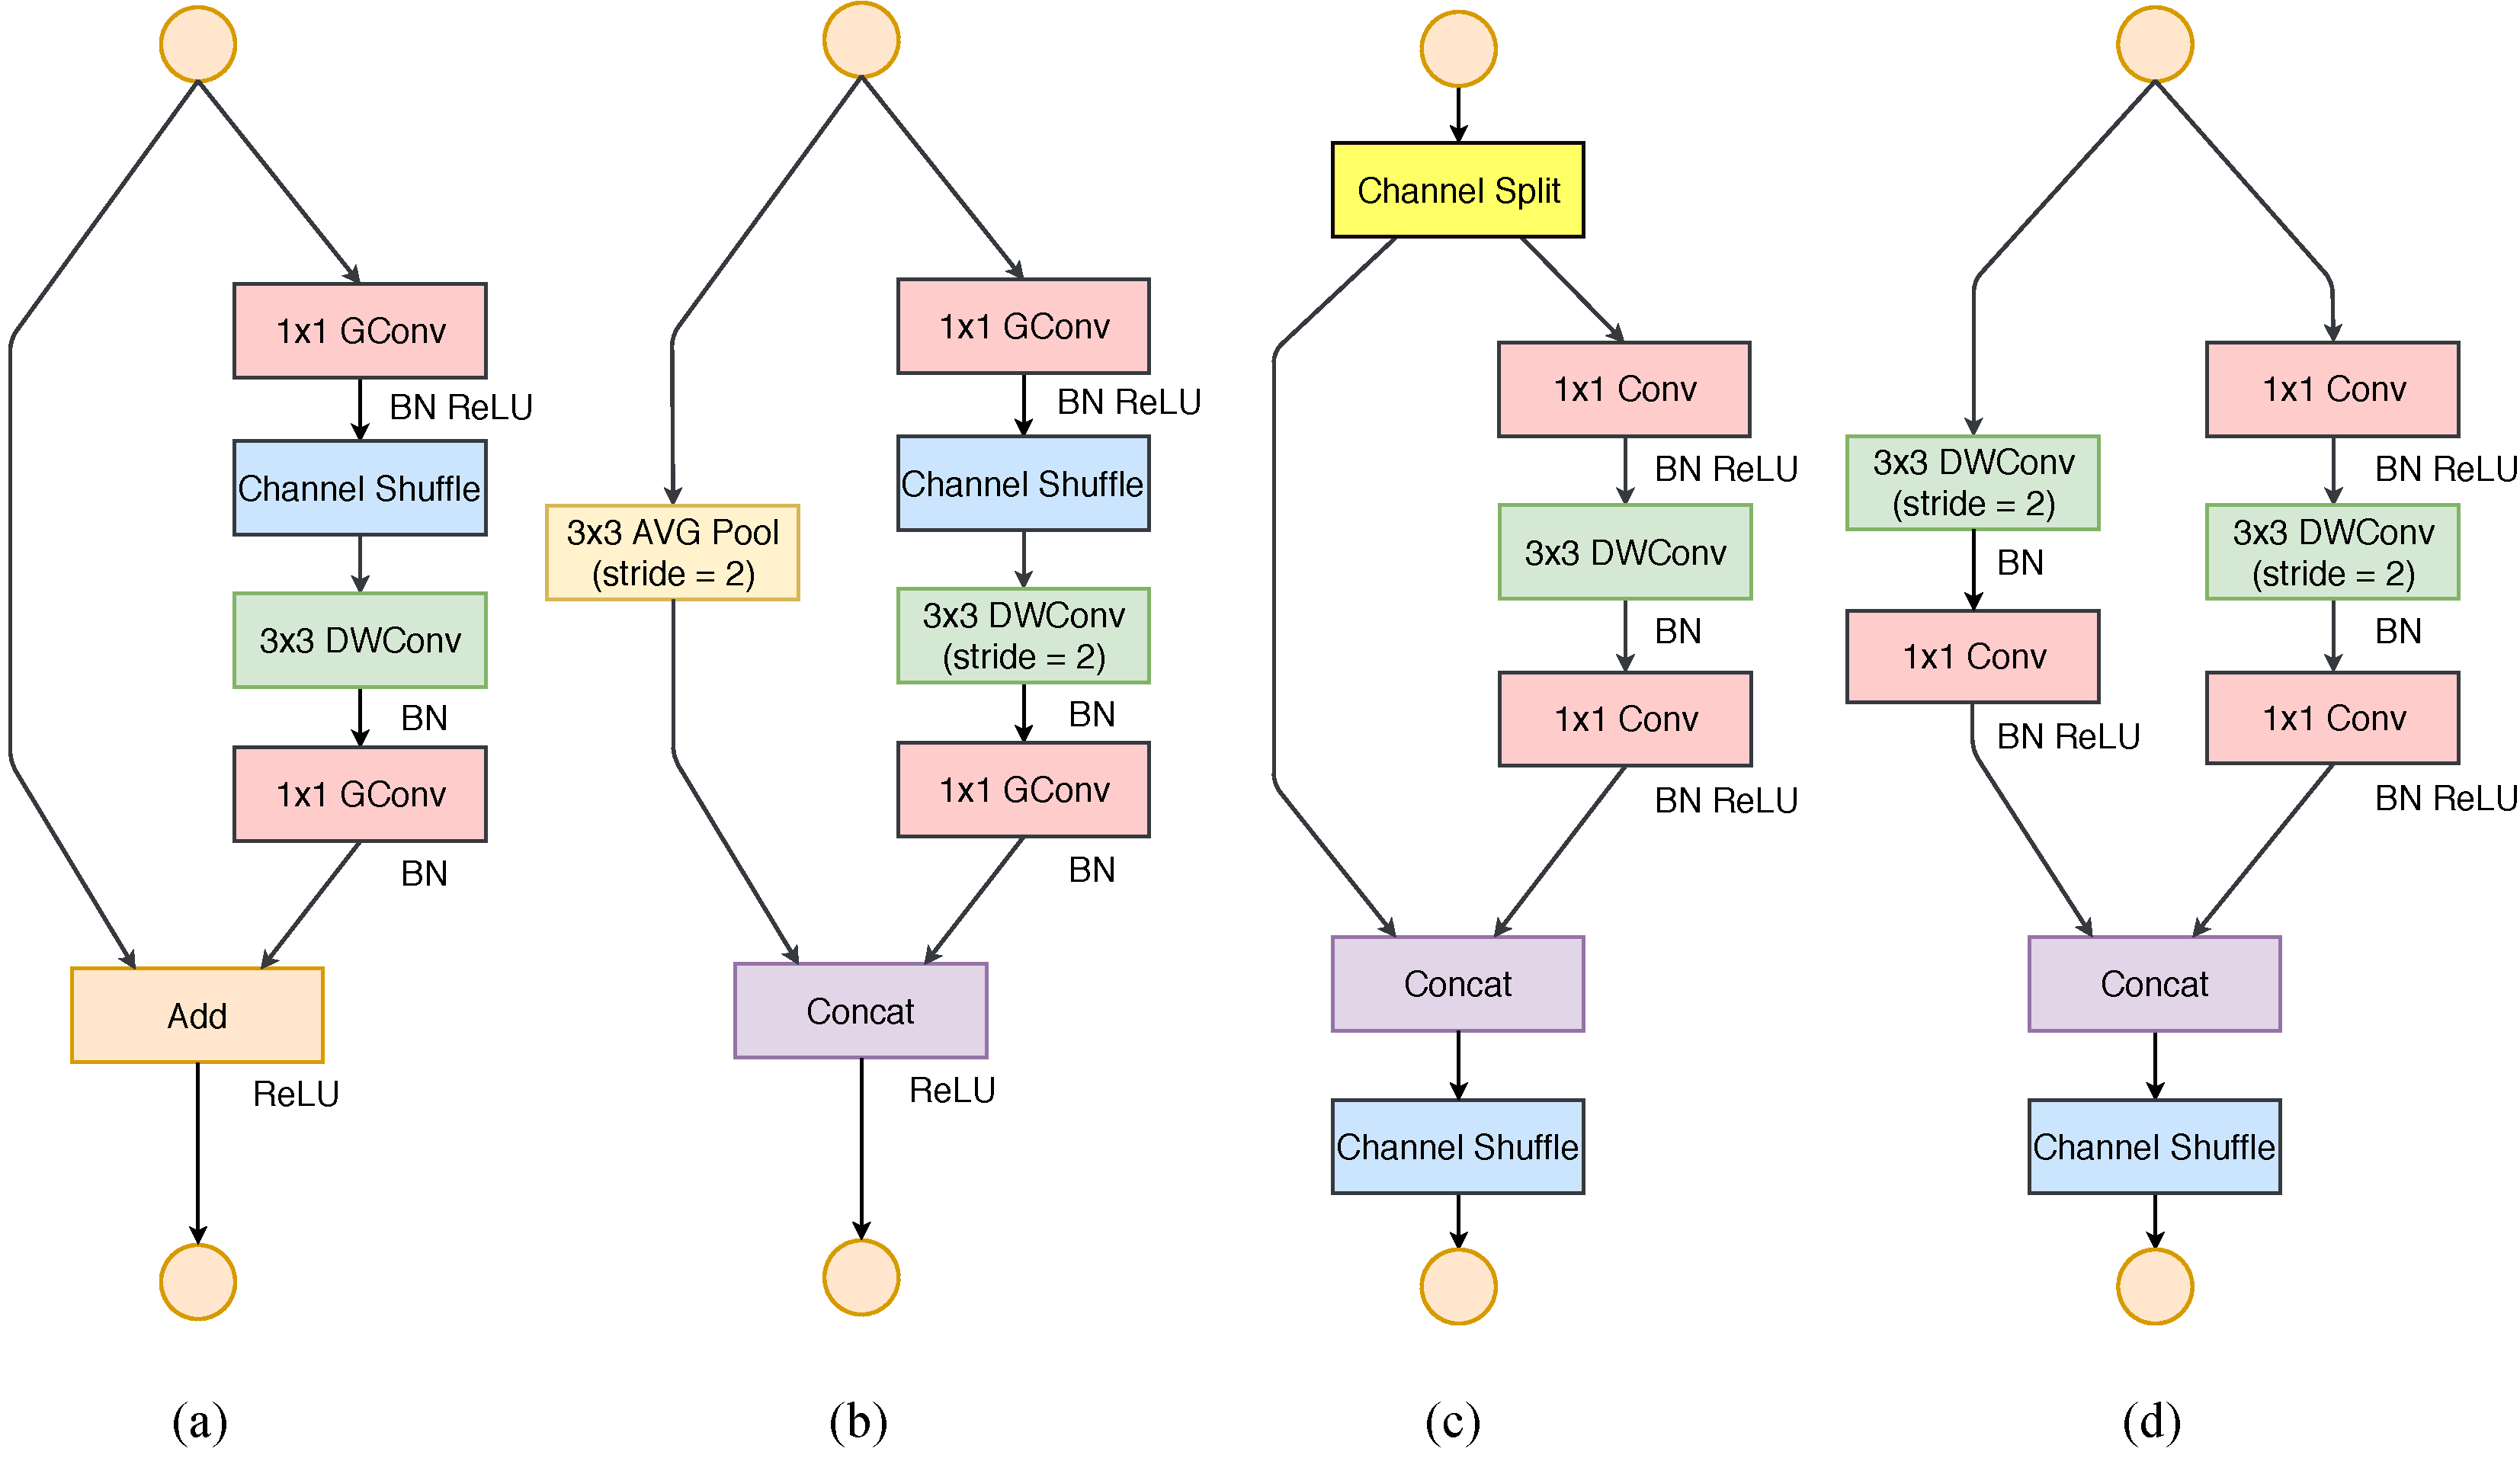
\includegraphics[width=\textwidth]{shufflenet.pdf}
    \caption{ShuffleNet结构}
    \label{fig:shufflenet}
\end{figure}

GhostNet\cite{han2020ghostnet}由华为诺亚方舟实验室提出,其核心思想在于提出了幻影模块(Ghost Module),该模块针对深度神经网络中存在的潜在冗余和相关性较高的特征图问题,通过高效的计算策略提炼出“幻影特征图”。研究团队发现,在许多情况下,多个特征图可能蕴含着相似的模式信息,这意味着部分特征图的信息实质上可以从其他特征图中推衍得出,犹如“幻影”。鉴于此,GhostNet摒弃了对每组特征图均采用标准卷积的传统做法,转而采用一种更为经济高效的计算方式去合成这类“幻影特征图”。在具体实施中,首先运用有限数量的标准卷积层提取基础特征图,以此严格控制参数规模,接下来通过对基础特征图施加一组精心设计的线性变换(通常是深度可分离卷积中的逐点卷积操作),高效地生成大量辅助特征图,这些辅助特征图被视为原始特征图的“幻影”。最后,Ghost模块将“幻影特征图”与标准卷积产生的少量核心特征图整合在一起,以有效模拟传统卷积所带来的丰富表征能力,在保持高精度的同时,降低了模型的计算复杂性和参数规模。Ghost模块的结构如图~\ref{fig:ghost}~所示,其中,Identity操作由标准卷积生成的特征图,\(\Phi\) 为廉价线性变换。
\begin{figure}
    \centering
    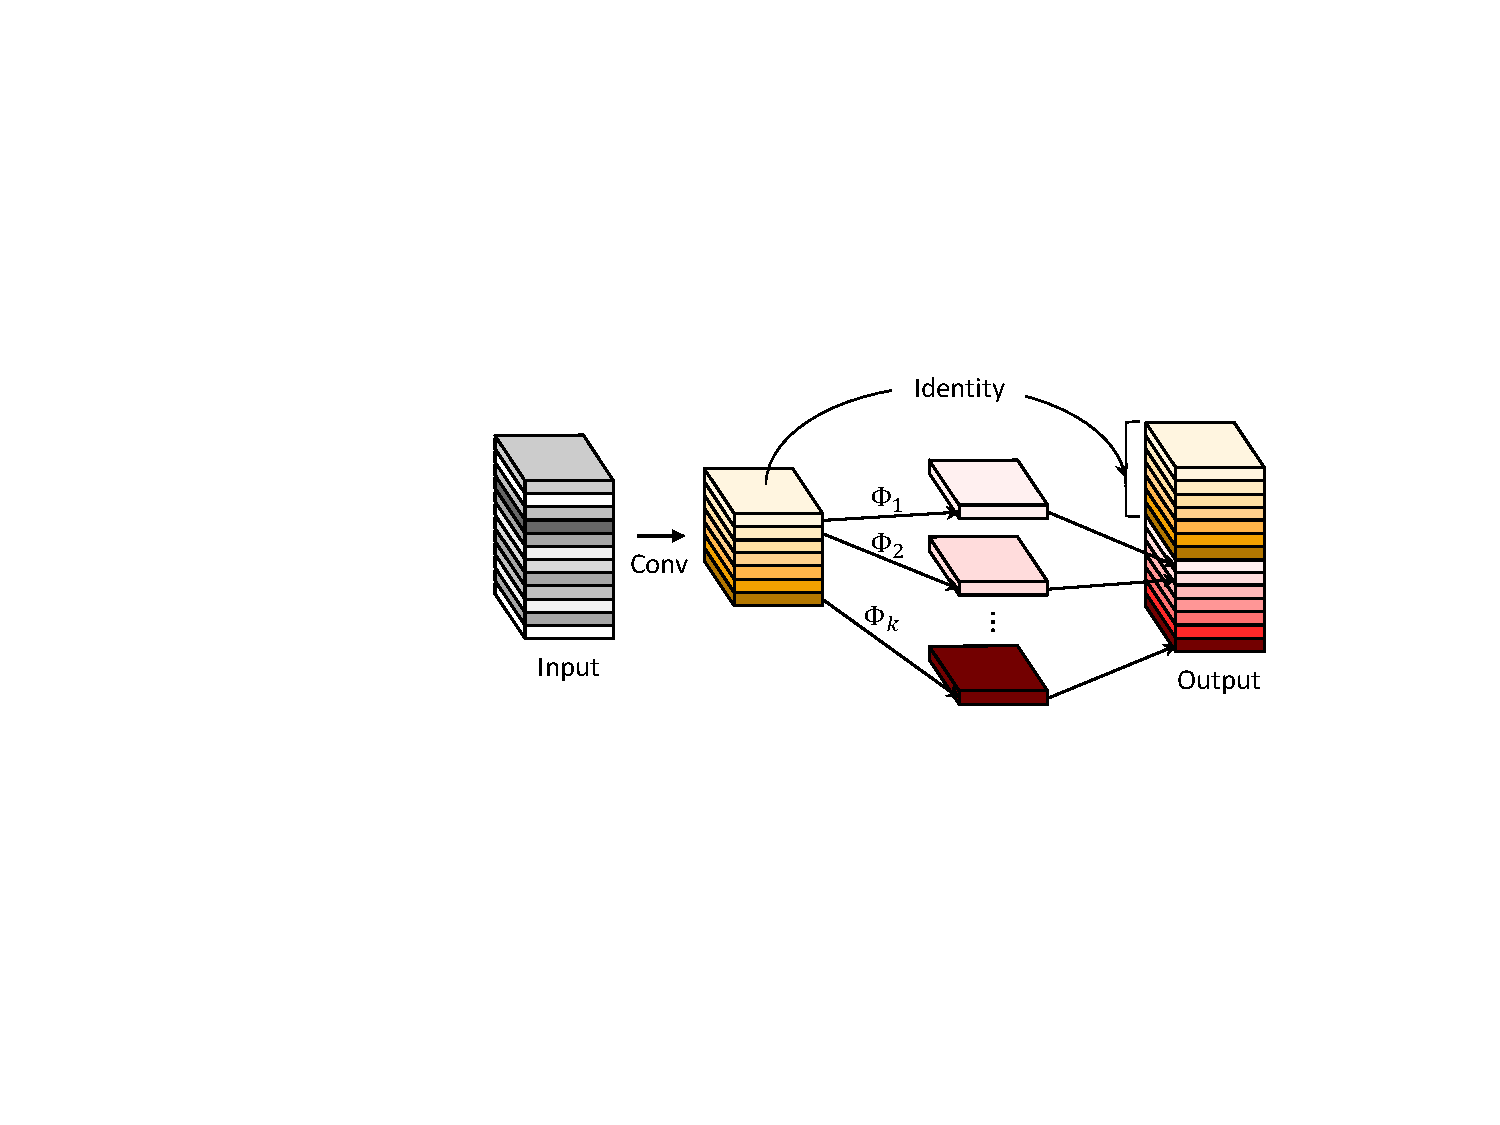
\includegraphics[width=\textwidth]{ghost.pdf}
    \caption{Ghost模块结构}
    \label{fig:ghost}
\end{figure}

\subsection{ShuffleNet结合GhostNet的轻量化卷积模块}

在HIT-Net架构中,已应用了诸如瓶颈层设计以及深度可分离卷积技术,从而有效地压缩了模型参数量。因此,本节在现有成果的基础上,主要结合ShuffleNetV2的基础单元和GhostNet所提出的Ghost模块进行了针对性改良。

ShuffleNetV2的优势体现在其利用通道混洗操作促进不同特征图组之间的信息交互,特别是在Channel Split机制中,它将特征图分割成两个部分,其中一个部分不经额外计算直接向下进行传递,这种设计有助于减少模型分支内的参数量。然而,ShuffleNetV2在进行Channel Split时,通常是对特征图进行均匀划分,这种方式难以灵活调整直传特征图的比例,可能导致对重要特征信息的有效利用率不足,并且在极端情况下可能影响模型精度。此外,ShuffleNetV2的基础结构在深度维度上的特征变换主要依赖于1×1卷积,这在一定程度上限制了其内在的深度特征变换能力。

为了提升ShuffleNetV2基本模块在深度特征变换方面的能力,论文提出了一种可调节分支比例的Shuffle模块(Adaptive Shuffle Module, AS模块),其架构如图(a)所示。假设卷积层的输入深度为 \(D_{in}\),输出深度为 \(D_{out}\),针对不同的输入输出深度关系(即 \(D_{in} \le D_{out}\) 和 \(D_{in} > D_{out}\) ),论文对AS模块进行了优化,分别形成了图(b)所示的GAS模块(Growing Adjustable Shuffle Module)和图(c)所示的SAS模块(Straight Adjustable Shuffle Module)。

对于GAS模块,在保留原有直接传递分支的同时,对进行深度变换的分支进行了如下改进:根据采样频率特性调整卷积核大小,为了描述的简洁性,以时间域特征提取卷积模块为例,并将其卷积核大小设定为1 \times 25,对于采样频率为250Hz的BCI Competition IV Dataset 2A数据集而言,意味着该卷积核以0.1秒的时间窗口进行特征捕获。进入变换分支的特征图首先通过1 \times 1卷积实现深度变换,紧接着通过1 \times 25的深度卷积进行特征提取,最后再次通过1 \times 1卷积将深度变换至输出需要的深度。在此过程中,加入了批归一化和GeLU激活函数。这样设计的目的是优化GAS模块对MI-EEG分类任务的性能。

对于权重参数为 \(ratio\) 的GAS模块,其直接传递分支的特征图输入数量 \(BS_{in}\) 设定为 \(BS_{in} = D_{in} \times ratio\),对应的输出数量 \(BS_{out}\) 同样为 \(BS_{out} = D_{in} \times ratio\)。而变换分支的特征图输入数量\(BT_{in}\) 则设定为 \(BT_{in} = D_{in} - BS_{in}\),其输出特征图数量 \(BT_{out}\) 计算为 \(BT_{out} = D_{out} - BS_{out}\)。这样的设计使得GAS模块能在维持模型轻量化的同时,更精准地针对MI-EEG分类任务进行深度特征提取与整合。

对于SAS模块,其在变换分支的设计上采用了与GAS模块一致的改进措施,但去掉了最后的1\times1卷积层,而由第一个1\times1卷积层将深度降维至输出维度,再由1\times25卷积层进行特征的提取。然而,在直接传递分支上,进一步引入了深度维度上的平均池化操作,目的在于在不增添额外参数的前提下,有效减少特征图的数量。SAS模块的池化分支的特征图输入数量 \(BS_{in}\) 设定为 \(BS_{in} = D_{in} \times ratio\),对应的输出数量 \(BS_{out}\) 设定为 \(BS_{out} = D_{out} \times ratio\)。而变换分支的特征图输入数量\(BT_{in}\) 则设定为 \(BT_{in} = D_{in} - BS_{in}\),其输出特征图数量 \(BT_{out}\) 计算为 \(BT_{out} = D_{out} - BS_{out}\)。相较于原始的Shuffle unit,GAS模块和SAS模块在功能上进行了扩展,不仅包含了特征维度的升维和降维处理,而且还引入了一个可调节的权重参数  \(ratio\),以动态控制两个分支的特征图数量。这样一来,这两种模块在处理MI-EEG分类任务时,能够更加灵活和高效地调整特征空间的分布和深度特征的提取,从而更好地适应任务需求和优化模型性能。

GhostNet的优势在于其Ghost模块设计,该模块凭借对特征图间内在相似性的有效利用,实现了低成本的特征转换操作。然而,Ghost模块在运用线性变换与传统卷积相结合的方式来产生新特征图的过程中,尚存在一定的局限性,即生成的特征图之间交互作用不充分。鉴于此,论文进一步改良了Ghost模块,引入了通道混洗机制,构建出SG模块(Shuffle Ghost Module)。SG模块的结构如图所示,通过通道混洗机制增强不同特征图之间的相互作用,进而提升网络的整体表现力和特征学习能力。此外,SG模块采用与GAS模块相同的方式对Ghost模块内部的卷积核大小进行了修改,并加入了批归一化和GeLU激活函数。

\section{基于MEKT算法改进的MI-EEG迁移学习算法SV-MEKT}


% chapter4 实验

\chapter{实验结果分析与模型评估}

\section{实验环境}

论文构建的HA-FuseNet是在实验室搭建的服务器上进行搭建和训练的,所用的软/硬件环境如表~\ref{tab:env}~所示:
\begin{table}[h]
    \centering
    \caption{实验环境}
    \label{tab:env}
    \begin{tabularx}{\textwidth}{>{\centering\arraybackslash\hsize=0.6\hsize}X >{\centering\arraybackslash\hsize=1.4\hsize}X}
    \toprule
    软/硬件名称 & 型号/版本 \\
    \midrule
    操作系统 & Ubuntu 20.04.6 LTS  \\
    CPU & Intel(R) Xeon(R) Gold 5218R CPU @ 2.10GHz \\
    GPU & NVIDIA GeForce RTX 3090 \\
    内存 & 128GB \\
    显存 & 24GB \\
    CUDA & 11.8 \\
    Python & 3.11.5 \\
    Pytorch & 2.0.1 \\
    MNE & 1.6.0 \\
    Numpy & 1.26.3 \\
    \bottomrule
    \end{tabularx}
\end{table}

\section{数据与实验准备}

\subsection{运动想象脑电图数据集}

运动想象脑电图是使用脑电采集设备从头皮上获取的人类大脑的神经元活动时产生的生物电电位信号,能够反映大脑皮层和深层结构的功能状态及其异常变化。脑电图信号的采集过程主要包括以下几个步骤:

(1) 采集准备:根据国际10-20标准导联系统或其他标准定位方案,将电极安放在被试头皮的不同位置,以捕获不同脑区的电位信号。电极通常通过电极帽或电极盘固定,以确保位置的稳定和正确。由于人体脑电信号强度微弱,通常会通过与脑电采集设备相连的放大器对脑电信号进行增强和记录;

(2) 信号记录:当大脑神经元兴奋或抑制时,会产生微弱的电位变化,这些电位变化传导到头皮表面,形成可测量的电压差,由脑电采集系统进行捕获和放大。脑电采集系统通常以每秒连续进行\(N\)次采集的方式工作,即采集频率为\(N\)Hz;

(3) 数字化:根据脑电采集系统的设置,对被捕获的脑电信号进行一定的处理,包括通过模数转换器(Analog to Digital Converter,ADC)将模拟信号转换为数字信号。

在临床和科研应用中,脑电图信号因其非侵入性、实时监测性、对大脑功能活动的敏感性等特点,已经在大脑解码领域获得了广泛的应用。运动想象领域有多个公开的脑电图信号数据集,论文主要选取BCI Competition IV Dataset 2A\cite{brunner2008bci}数据集和BCI Competition IV Dataset 2B\cite{leeb2008bci}数据集作为模型训练和测试的数据集。BCI Competition(脑机接口竞赛)是一项由德国柏林洪堡大学和柏林工业大学发起的国际性脑机接口技术竞赛,旨在推动脑机接口技术的创新和发展。在第四届比赛(BCI Competition IV)中,主办方提供了多项数据集,其中,运动想象领域的2A和2B数据集在相关研究中被广泛使用。

\paragraph{BCI Competition IV Dataset 2A}

BCI Competition IV Dataset 2A数据集采集了9名被试的MI-EEG信号,包括4类运动想象任务,即左手、右手、双脚和舌头。每名被试在不同的日期进行了两次采集/会话(session),两个session分别被作为训练集(T)和测试集(E),数据以.gdf的格式存储,因此,每名被试具有两个文件,如对于一号被试而言,存在A01T.gdf和A01E.gdf两个文件,其中,训练集A01T.gdf包含标签信息,A01E.gdf不包含标签信息,使用额外的A01E.mat文件提供标签。

session采集的过程如图~\ref{fig:2asession}~所示,在采集开始时,进行约五分钟的EOG记录,包括两分钟的睁眼模式、一分钟的闭眼模式和一分钟的眼球运动模式。其中,四号被试的测试集只具有眼球运动的EOG记录。
\begin{figure}
    \centering
    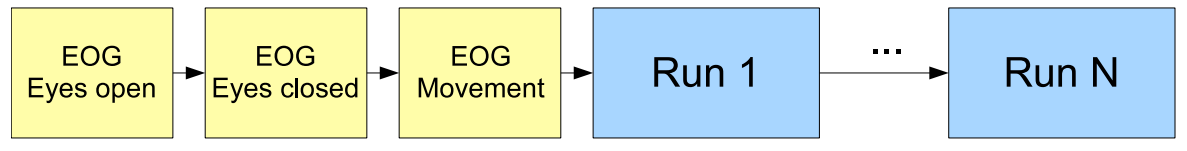
\includegraphics[width=0.8\textwidth]{2asession.png}
    \caption{2A session采集模式\cite{brunner2008bci}}
    \label{fig:2asession}
\end{figure}

在EOG记录之后,进行六次采集(run),在每个run中,各进行12次每类运动想象任务,这些任务的顺序是随机的,由此,一个run包含48次试验(trial),一个session包含288次试验(trial)。一个trial的流程如图~\ref{fig:2atrial}~所示,测试开始时(t=0s),一个十字图形出现在屏幕上,伴有简短的提示音;两秒后(t=2s),运动想象任务的指示箭头(分别指向左、右、下、上,对应左手、右手、双脚及舌头运动)出现在屏幕上,持续约1.25秒,每名被试进行运动想象任务直到十字图形消失(t=6s)。在这个过程中没有任何反馈。
\begin{figure}
    \centering
    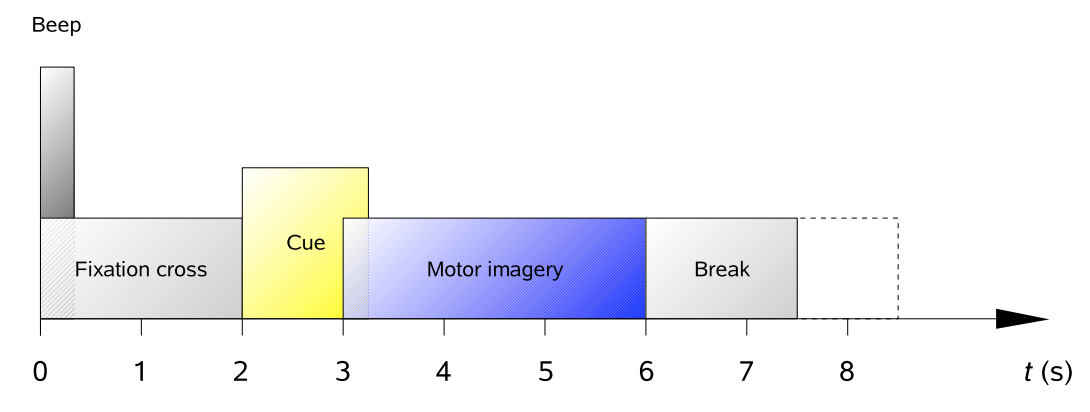
\includegraphics[width=0.8\textwidth]{2atrial.png}
    \caption{2A trial与无视觉反馈的2B trial的采集模式\cite{brunner2008bci,leeb2008bci}}
    \label{fig:2atrial}
\end{figure}

采集过程中,以250Hz进行EEG信号采样,并在0.5Hz至100Hz之间进行了带通滤波,放大器的灵敏度被设置为100\(\mu\)V,并使用了50Hz的陷波滤波器用以抑制线路噪声。头皮电极的位置按照国际10-20标准导联确定,共使用22个电极(通道),此外,还使用了3个不参与分类的EOG电极用以记录眼电信号。

在BCI领域,事件描述某一种波形或任务的起始点,数据上,事件表现为一个三元组:第一个元素以整数来描述的事件起始采样点;第二个元素对应当前事件来源的刺激通道(Stimulus Channel)的先前值(Previous Value),大多数情况下为0;第三个元素表示该事件的类型(Identify,id)。BCI Competition IV Dataset 2A数据集中共包含11类事件(Event),其中,与数据处理相关的事件如表~\ref{tab:2aevent}~所示,其中,拒绝试验是指由于质量欠佳或受试者未能有效完成而被专家标注出的试验数据。
\begin{table}[h]
    \centering
    \caption{2A事件类型列表}
    \label{tab:2aevent}
    \begin{tabularx}{\textwidth}{CC}
    \toprule
    事件类型 & 描述 \\
    \midrule
    768 & trial开始  \\
    769 & 左手运动想象任务(class 1) \\
    770 & 右手运动想象任务(class 2) \\
    771 & 双脚运动想象任务(class 3) \\
    772 & 舌头运动想象任务(class 4) \\
    783 & 未知运动想象任务(测试集) \\
    1023 & 拒绝试验 \\
    \bottomrule
    \end{tabularx}
\end{table}

论文遵循BCI Competition竞赛设置,使用T文件为训练集,E文件为测试集,针对每名被试进行被试内实验和被试间实验。则在不剔除拒绝试验数据的情况下,每名被试的训练集和测试集切片数量分别为:288,288。

\paragraph{BCI Competition IV Dataset 2B}

BCI Competition IV Dataset 2B采取了类似2A数据集的采集方式,采集了9名被试的2类MI-EEG信号(左手、右手),每名被试在不同时间进行了五次session,数据以.gdf格式存储,每名被试有五个文件,例如,对于一号被试而言,B0101T.gdf、B0102T.gdf和B0103T.gdf为训练集,、B0104E.gdf和B0105E.gdf为测试集。其中,前两个文件不包含视觉反馈,后三个文件包含视觉反馈,即在试验过程中,通过屏幕上的笑脸图案对运动想象任务是否被正确执行予以反馈。无视觉反馈的session包含6次run,每个run包含20次trial(左手、右手各10次,随机排布),有视觉反馈的session包含4次run,每个run包含40次trial(左手、右手各20次,随机排布)。无视觉反馈的trial的采集模式与2A相同,如图~\ref{fig:2atrial}~所示。

BCI Competition IV Dataset 2B的事件类型与2A的事件类型相似,但不包含双脚和舌头运动想象任务。此外,不同于2A数据集的22个电极,2B数据集仅使用3个电极记录数据。

为了保证实验数据只涉及运动想象,而不涉及视觉反馈,论文选择无视觉反馈的两个session分别作为训练集和测试集,则在不剔除拒绝试验数据的情况下,每名被试的训练集和测试集切片数量分别为:120,120。

综上所述,论文所使用的数据的信息如表~\ref{tab:dataset}~所示。
\begin{table}[ht]
    \centering
    \caption{数据集信息}
    \label{tab:dataset}
    \begin{tabularx}{\textwidth}{CCC}
      \toprule
      数据集 & BCI IV 2A & BCI IV 2B \\
      \midrule
      被试数量 & 9 & 9 \\
      类别数量 & 4 & 2 \\
      通道数量 & 22 & 3 \\
      频率范围 & 0.5-100Hz & 0.5-100Hz \\
      采样频率 & 250Hz & 250Hz \\
      训练集数据量 & 288(每被试) & 120(每被试) \\
      测试集数据量 & 288(每被试) & 120(每被试) \\
      \bottomrule
    \end{tabularx}
\end{table}

\subsection{数据预处理}

EEG信号具有低信噪比、非平稳、空间变异性等特性,并且通常具有较小规模的数据集,一般来说,对数据进行一定的预处理有助于后续分类任务。然而,论文基于端到端网络的思想构建模型,因此尽可能地对预处理操作进行削减。论文进行的数据预处理操作如下:

\paragraph{数据提取与切片}

MI-EEG原始信号储存在.gdf格式的文件中,除目标脑电信号之外,原始文件还包括EOG信号、间隙缺失值、与运动想象任务不直接相关的事件等。因此,在提取数据时,有必要进行一定的处理:

首先,剔除EOG通道数据,仅保留EEG通道数据,对于用于分隔run的缺失值(编码为非数字,NaN),使用对应通道的均值替代,以确保数据的连续性和完整性;

其次,对与运动想象任务直接相关的事件进行筛选和提取,并对相关时段进行切分。对于BCI Competition IV的2A/2B数据集,直接相关事件为四类/二类运动想象任务事件,并由提示信号(Cue)标识任务的开始,论文对连续数据进行切片,提取从Cue出现后的第1秒至第4秒(trial周期的第3秒至第6秒)的数据段,作为事件对应的运动想象任务持续期间产生的EEG信号,在后续加以分析。对于采样率为250Hz的数据集而言,3秒的数据区间将包含750个采样点。

需要说明的是,论文在数据提取过程中并未对拒绝试验进行剔除,同时未使用滤波器对EEG信号的频率进行过滤,以对真实应用情境中可能出现的多样化数据表现进行模拟,对模型自主识别各种频率成分并提取有效特征的能力进行评估。

\paragraph{标准化}

归一化操作的目的在于对数据的特征尺度进行统一,从而消除奇异数据导致的不良影响,提高模型的训练效率和稳定性。Z-score标准化、最大最小值归一化等方法是EEG信号处理中经典的算法。

经过Z-score处理的数据为标准正态分布,其操作过程如公式~\ref{eq:z-score}~所示,其中,\(x\)为原始数据,\(\mu\)表示\(x\)的均值,\(\sigma\)表示\(x\)的标准差。
\begin{equation}
    x=\frac{x-\mu}{\sigma}
    \label{eq:z-score}
\end{equation}

最大最小值归一化的操作过程如公式~\ref{eq:maxmin}~所示,其是一种线性变换操作,将数据映射至\([0,\,1]\)区间,其中,\(X\)为一组通道数据。最大最小值归一化计算简单,但对具有波动性的EEG信号而言,将数据缩放至\([0,\,1]\)区间容易导致数据特征的损失。
\begin{equation}
    x=\frac{x-min(X)}{max(X)-min(X)}
    \label{eq:maxmin}
\end{equation}

因此,为了尽可能保留EEG信号的特征,论文应用Z-Score方法处理EEG信号,进行标准化,以提高模型训练的速度和稳定性。

\paragraph{数据增强}

MI-EEG信号通常具有较小规模的数据集,因此,通过一定的数据增强操作扩大数据规模,有助于提升网络训练效果,防止过拟合现象的发生。然而,在BCI系统的实际应用中,数据增强操作可能会导致训练阶段数据处理压力的增长,因此,在论文中,数据增强是一项可选操作,其目的在于提高模型分类精度,论文将分别使用进行数据增强和不进行数据增强的数据集进行训练。

EEG信号的数据增强方法主要有以下几种:

(1) 添加随机噪声:在EEG信号上叠加高斯白噪声、有色噪声等不同类型的噪声,模拟真实环境中的噪声干扰,能够提升模型的抗噪性和鲁棒性;

(2) 滑动窗口:设定时间滑动窗口的长度小于运动想象任务持续的时间长度,将滑动窗口内的数据视作一次事件,通过滑动窗口对数据进行切片,有助于模型学习EEG信号随时间变化的特征;

(3) 频率混叠:在保持EEG信号特性的前提下,将多种不同频率成分进行混叠,使得模型能够学习更广泛的频率特征。

由于在预处理阶段没有采取频率滤波的操作,论文采取频率混叠的方式对EEG信号进行增强,从而加强模型识别不同频率成分的能力。具体算法流程如算法~\ref{alg:aug}~所示。
\begin{algorithm}[H]\label{alg:aug}
    \caption{数据增强算法}
    \SetAlgoLined
    \KwData{Dataset for every subject $X=\{x_1, x_2, ..., x_9\}$ and the $subject\_id$ to be augmented.}
    \KwResult{augmented dataset for every subject $Y=\{y_1, y_2, ..., y_9\}$.}
    $Y = []$ \;
    \For{each item $x_i \in X$}{
        $X' = $ selected $x_j$ from $X,\,j \neq i,\,j \in [1,2,...,9]$ \;
        $y_i = x_i$ \;        
        $x_i = $ crop $x_i$ from where the first trial begins\;
        $x_i = $ filter $ x_i $ into $ [4Hz,40Hz] $ \;
        \For{each item $s_i \in X'$}{
            $s_i = $ crop $s_i$ from where the first trial begins\;
            $s1_i = $ filter $ s_i $ into $ [0.5Hz,4Hz)$ \;
            $s2_i = $ filter $ s_i $ into $ (40Hz,100Hz)$ \;
            $y_i = $ concatenate $ (y_i, s1_i+x_i+s2_i)$ \;
        }
        $Y = Y$ append $y_i$ \;
    }
    \Return{$Y$}\;
\end{algorithm}

\subsection{实验准备}

\paragraph{评价指标}

论文主要使用准确率(Accuracy,Acc)、Kappa一致性系数(Kappa)和标准差(Standard Deviation,SD)作为模型的评价指标。其中,准确率是分类任务中常用的评价指标,用于衡量模型预测结果与真实标签相匹配的比例,其计算方式为总样本中,分类正确的样本的比例。

Kappa一致性系数用于衡量模型预测结果与真实标签之间的一致性程度,在类别不平衡或随机猜测具有一定效果的情况下,Kappa一致性系数尤其有效。Kappa系数基于混淆矩阵进行计算,其计算公式如下:
\begin{equation}\label{eq:kappa}
    Kappa=\frac{P_o-P_e}{1-P_e}
\end{equation}
其中,\(P_o\)为观察一致性(Observed Proportion of Agreement),即准确率,\(P_e\)为预期一致性(Expected Proportion of Agreement by Chance),假设样本总量为\(N\),类别总量为\(c\),第\(i\)类的真实样本个数为\(x_i\),预测样本个数为\(p_i\),则\(P_e\)的计算公式如~\ref{eq:pe}~所示。
\begin{equation}\label{eq:pe}
    P_e=\frac{\sum_{i=1}^{c}x_i \times p_i }{N^{2} } 
\end{equation}
Kappa系数的范围在-1至1区间内,通常大于0,Kappa值越大,表明一致性程度越高,当Kappa值位于[0.61,0.80]区间时,表示预测与真实具有高度的一致性。

标准差为准确率的标准差,用于衡量模型在不同被试之间的稳定性能力,其值越小,表明不同被试的准确率越相近,模型在不同被试间的性能表现越稳定。准确率标准差的计算方式如下:
\begin{equation}
    SD=\sqrt{\frac{1}{N-1}  \sum_{i=1}^{N}(x_i-\bar{x} )^{2} } 
    \label{eq:sd}
\end{equation}
其中,\(N\)表示被试数量,\(x_i\)表示第\(i\)个被试的准确率,\(\bar{x}\)为\(N\)个被试准确率的平均值。

\paragraph{损失函数及参数配置}

论文使用交叉熵损失函数(Cross Entropy Loss)。交叉熵用于度量预测概率分布与实际概率分布之间的不一致,其值越小,表明两个概率分布越相似,因此,可以通过最小化交叉熵的方式,使得一个概率分布逼近目标概率分布。

交叉熵损失函数是一类在分类任务中广泛应用的损失函数,能够衡量模型预测值与真实标签之间的差异,其计算公式如下:
\begin{equation}
    L= -\sum_{i=1}^{C}y_i log(\hat{y}_i )
    \label{eq:loss}
\end{equation}
其中,\(C\)为分类类别数,\(y_i\)表示真实类别,\(\hat{y}_i\)表示模型预测的类别\(i\)的概率。交叉熵损失函数使用真实标签对模型预测的结果进行惩罚,从而促使模型学习到更为准确的预测结果。

论文使用Adam优化算法。对于2A数据集,批大小设置为32,2B数据集设置为20;实验迭代次数设置为300次;学习率的初始值设置为1e-3,权重衰减值设置为5e-3。

\section{实验设计}

\subsection{DIS-Net实验设计}

为了确定模型架构的最佳设置,本节对DIS-Net构建过程中不同的模型架构进行实验,从而逐步构建起性能最优的模型。

\paragraph{Inception模块引入空间卷积层的方式}

在DI-Net中,空间卷积层有两种不同的方式融入基于Inception改进的时间卷积层之后,一种是在每个Inception模块内部的分支结构上增加空间卷积层,另一种则是在整个Inception模块之后附加空间卷积层。图~\ref{fig:ts-incep}~展示了这两种引入方式的区别,将这两种方式分别称为分支内融合(Inception-In)和模块后融合(Inception-After),需要说明的是,图中省略了网络的其他结构,如瓶颈层等,以尽可能简洁地展现不同引入方式的差异。其中,\(s\_kernel\)表示空间卷积核,\(t\_kernel_i\)表示第\(i\)个分支的时间卷积核。
\begin{figure}
  \centering
  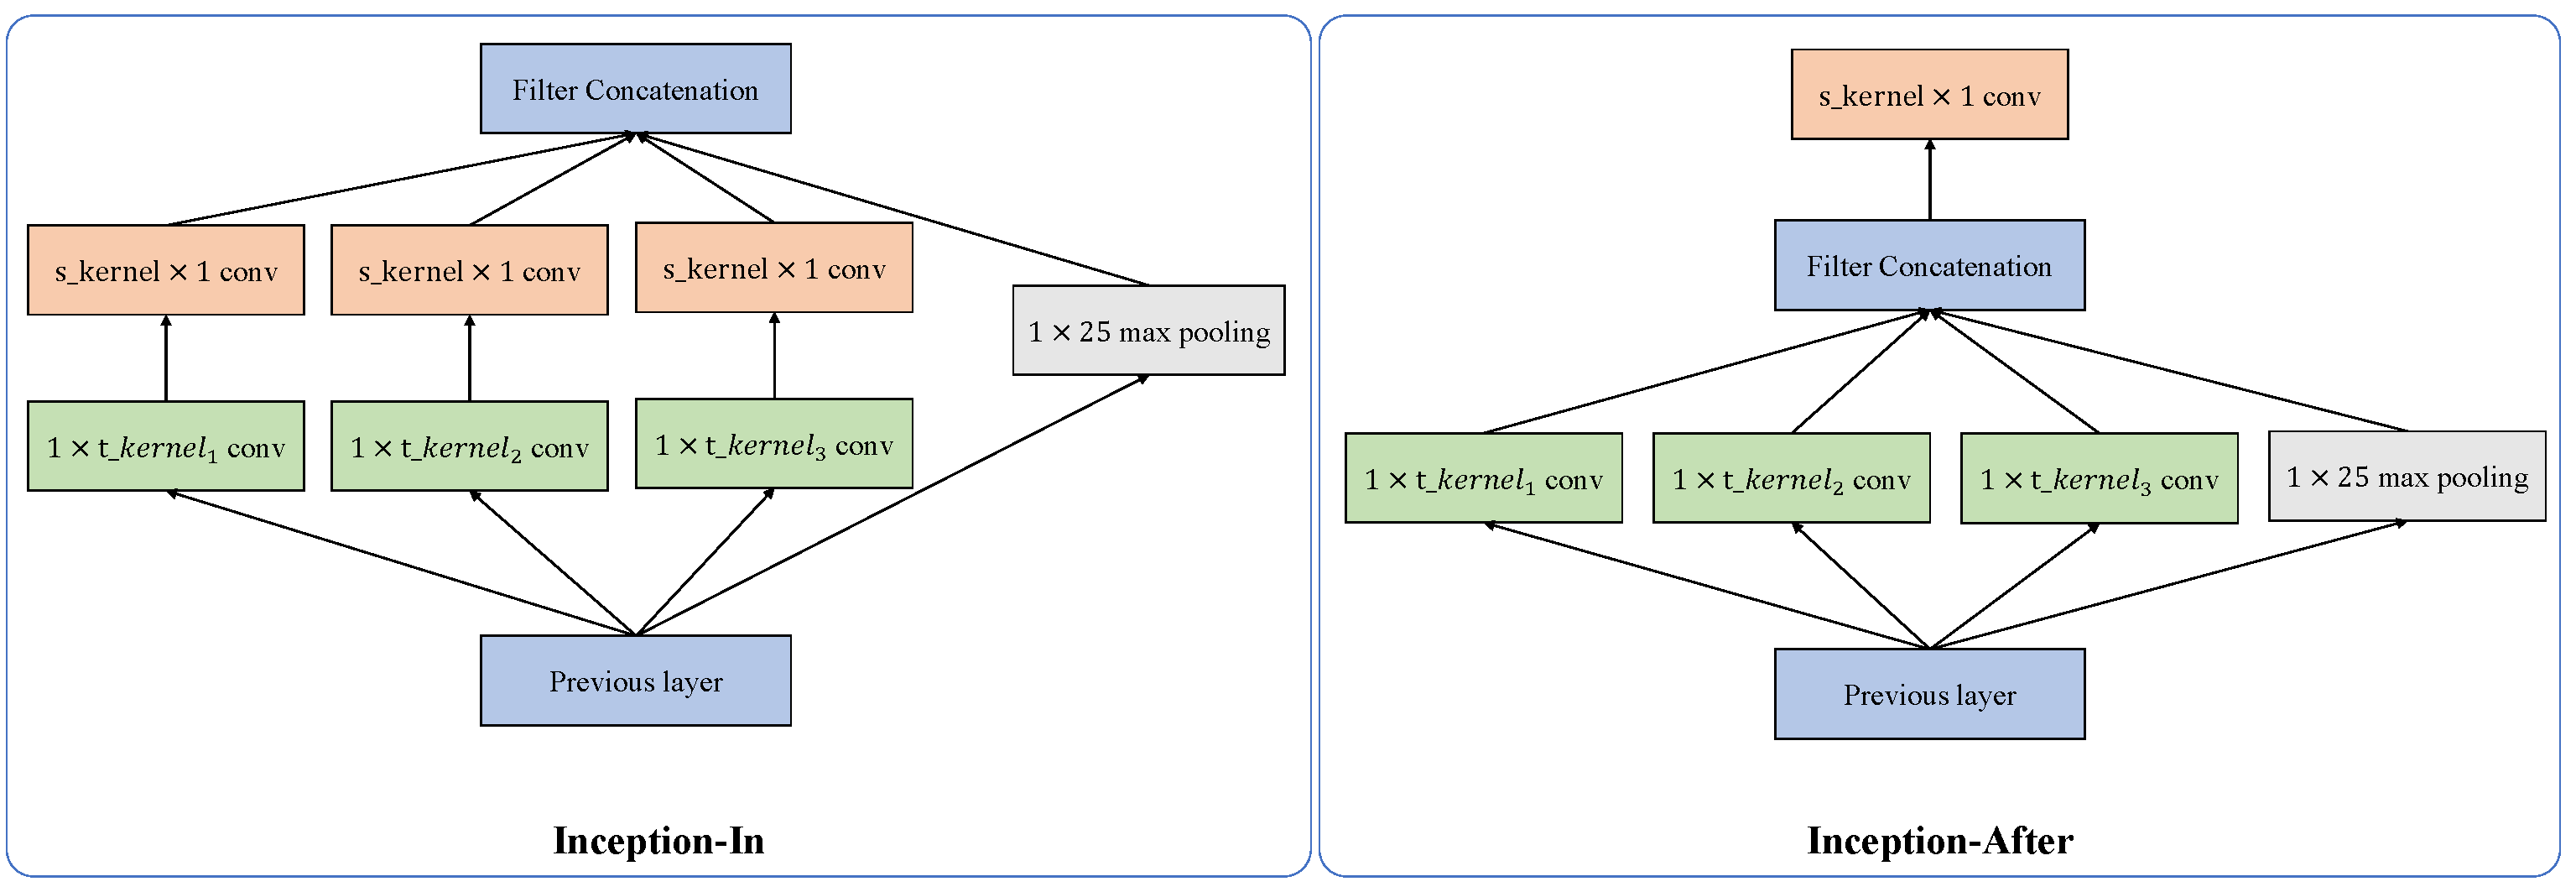
\includegraphics[width=\textwidth]{ts-incepv3.pdf}
  \caption{Inception模块引入空间卷积层的方式}
  \label{fig:ts-incep}
\end{figure}

为了比较Inception-In与Inception-After的性能差异,论文在BCI Competition IV Dataset 2A数据集上设计实验进行对比。在实验设置阶段,固定了Inception模块的层次数量、分支数量等参数,实验结果如表~\ref{tab:ts-inception}~所示。表格中的两项指标均基于数据集中九位被试的平均表现。实验结果显示,Inception-After方式在准确率和一致性系数上均表现更优。这一优势可能源自两方面的原因:一方面,虽然Inception-In模式借鉴了FBCSP算法的分频段处理思路,但在Inception分支内部直接进行空间特征提取的过程中,损失了部分空间全局信息;另一方面,Inception-In结构具有相对更大的参数规模,这可能导致模型在有限样本条件下更容易出现过拟合现象。基于以上分析和实验验证,论文选择以Inception-After的方式布局时间卷积层与空间卷积层。
\begin{table}[ht]
  \centering
  \caption{Inception-In、Inception-After实验结果对比}
  \label{tab:ts-inception}
  \begin{tabularx}{\textwidth}{CCC}
    \toprule
    Models & ACC(\%) & Kappa \\
    \midrule
    Inception-In & 69.01 & 0.58 \\
    Inception-After & \textbf{74.42} & \textbf{0.65} \\
    \bottomrule
  \end{tabularx}
\end{table}

\paragraph{svSE模块引入的对比实验}

为了选择适合MI-EEG分类任务的基准注意力机制,论文在DI-Net引入了不同的混合注意力模块,并在2A数据集上进行了实验,实验结果如表~\ref{tab:att}~所示,表中的指标为九位被试的平均表现。数据显示,scSE模块取得了最好的表现,因此论文选择基于scSE模块进行改进。
\begin{table}[ht]
    \centering
    \caption{不同注意力模块引入DI-Net的实验结果对比}
    \label{tab:att}
    \begin{tabularx}{\textwidth}{CCC}
      \toprule
      Attention & ACC(\%) & Kappa \\
      \midrule
      CBAM\cite{woo2018cbam} & 74.97 & 0.64 \\
      scSE\cite{8578843} & \textbf{75.35} & \textbf{0.67} \\
      CoordAttention\cite{Hou2021CoordinateAF} & 73.82 & 0.62 \\
      \midrule
      svSE & 76.16 & 0.68 \\
      \bottomrule
    \end{tabularx}
\end{table}

在表~\ref{tab:att}~中,同样展示了svSE以同样方式引入DI-Net的效果,svSE在四类混合注意力机制中取得了最高的准确率和Kappa系数,证明了svSE模块改进的有效性。

DIS-Net中,由于DI-Net的特征提取过程分为时间卷积和空间卷积两个阶段,svSE模块可采取以下三种引入方式:其一是在时间卷积层后引入;其二是在空间卷积层后引入;其三是同时在时间卷积层和空间卷积层之后引入。图~\ref{fig:att-Base}~展示了这三种引入svSE模块的方式,从左至右分别是时间卷积层后引入svSE模块、空间卷积层后引入svSE模块,以及在时间卷积和空间卷积层后均引入svSE模块。将这三种引入方式对应的模型分别简称为S-Temporal-Net、S-Spatial-Net、S-TS-Net。
\begin{figure}
  \centering
  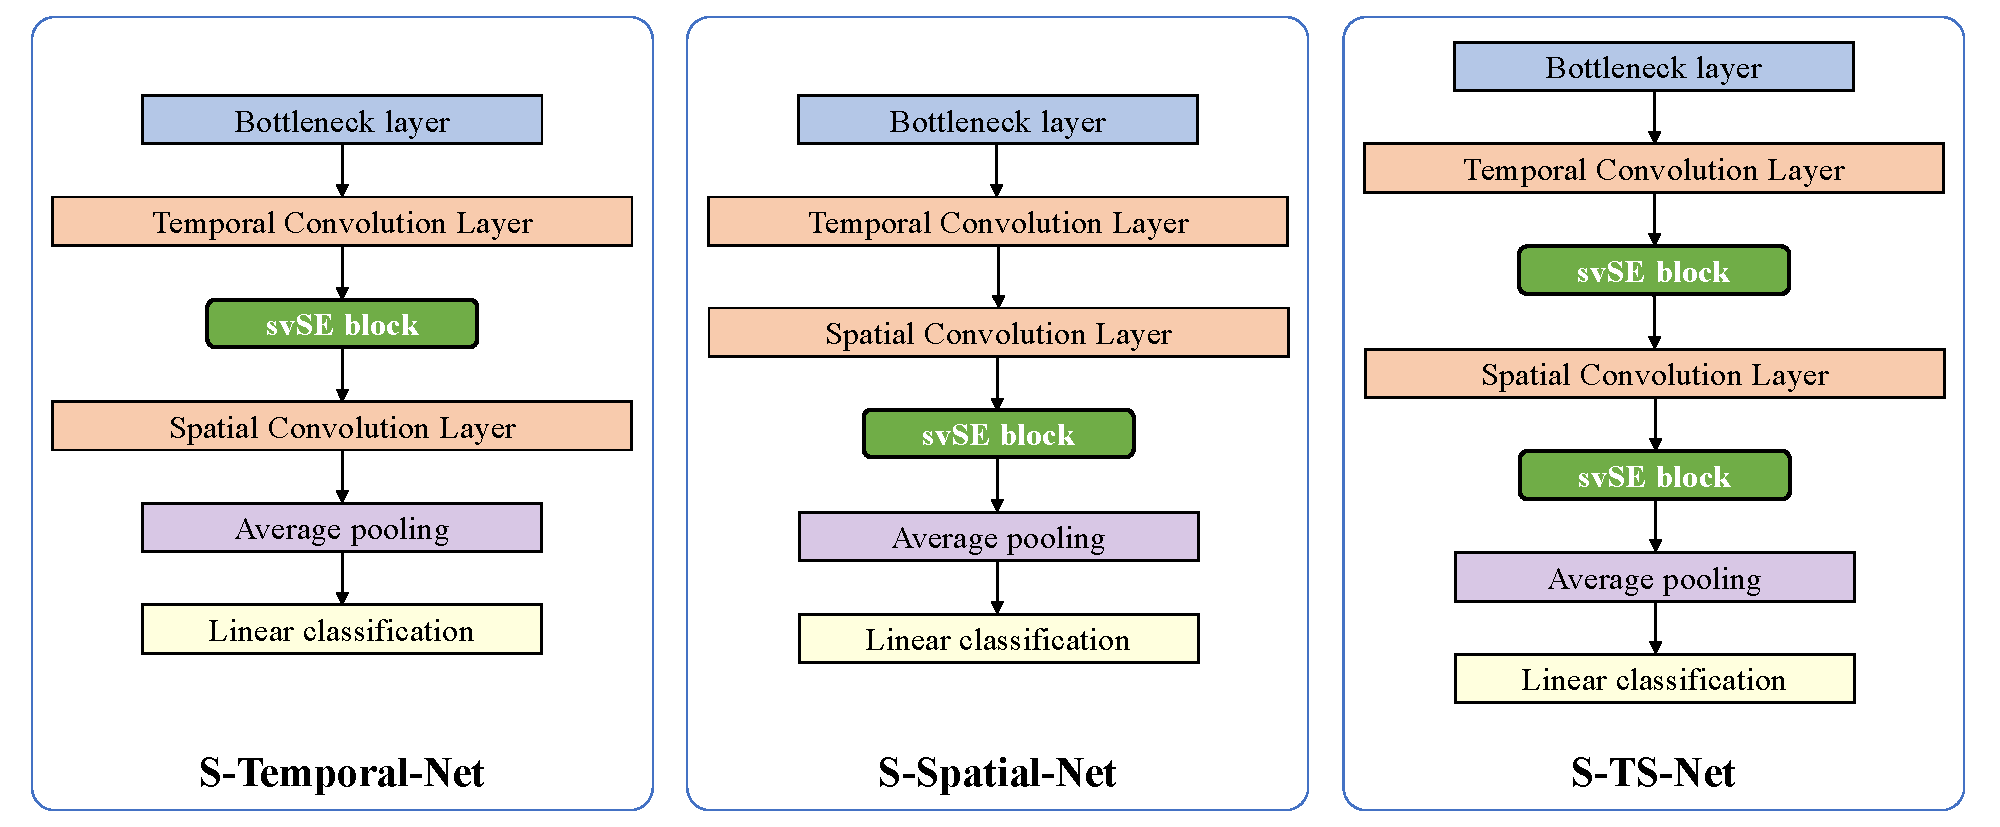
\includegraphics[width=\textwidth]{att-Basev2.pdf}
  \caption{DI-Net引入注意力模块的方式}
  \label{fig:att-Base}
\end{figure}

表~\ref{tab:svSE-BaseNet}~展示了S-Temporal-Net、S-Spatial-Net、S-TS-Net三种模型在2A数据集上的对比实验结果。表格中的指标为数据集中九位被试的平均表现。从准确率和一致性分析,S-ST-Net模型的效果优于其他两种模型,与经验相符。此外,S-Temporal-Net模型的效果优于S-Spatial-Net模型,其原因可能在于,空间卷积层沿通道维度的卷积使得数据损失了部分特征,进而减弱了svSE模块提取关键特征权重的能力,而时间卷积层保留了大部分深度信息和通道信息,因此,在时间卷积层之后加入svSE模块能够帮助模型更好地捕捉深度和空间的特征。从标准差分析,S-TS-Net模型的准确率波动幅度较小,对不同被试的MI-EEG分类效果相对均衡,另外两种模型在不同被试间的分类精度则存在较为明显的差异。实验数据显示,S-TS-Net模型取得了更好的效果,因此,论文采用了同时在时间卷积层和空间卷积层之后引入svSE模块的方式,即DIS-Net。
\begin{table}[ht]
    \centering
    \caption{svSE模块引入位置对比}
    \label{tab:svSE-BaseNet}
    \begin{tabularx}{\textwidth}{CCCC}
        \toprule
        Models & ACC(\%) & Kappa & SD \\
        \midrule
        S-Temporal-Net & 76.09 & 0.68 & 11.57 \\
        S-Spatial-Net & 75.03 & 0.66 & 11.88 \\
        S-TS-Net & \textbf{76.16} & \textbf{0.68} & \textbf{11.33} \\
        \bottomrule
    \end{tabularx}
\end{table}

\paragraph{不同轻量化模块对比}

为了验证更适合的轻量化卷积模块,论文在BCI Competition IV Dataset 2A数据集上进行了实验验证。由于轻量化卷积主要针对密集连接进行改进,实验使用DI-Net,并固定了Inception层数、密集连接层数、\(ratio\)等超参数。对\(ratio\)进行固定而非设置为可训练参数的原因是控制模块参数量的大小,避免轻量化卷积模块向原始密集连接模块趋近。表~\ref{tab:lite}~展示了ShuffleNet、GhostNet、SG和原始密集连接(Origin)模块的对比实验结果,其指标为参数量(Parameters)、浮点运算数(Floating Point Operations,FLOPs)和准确率,其中,准确率为九位被试的平均值。
\begin{table}[ht]
    \centering
    \caption{轻量化卷积模块实验结果对比}
    \label{tab:lite}
    \begin{tabularx}{\textwidth}{CCCC}
      \toprule
      Models & Paramters & FLOPs & ACC(\%) \\
      \midrule
      ShuffleNet & 7.31K & 130.37M & 72.96\\
      GhostNet & \textbf{7.27K} & \textbf{129.93M} & 73.14\\
      SG & 7.36K & 133.04M & \textbf{73.71}\\
      \midrule
      Origin & 29.99K & 690.37M & 74.42\\
      \bottomrule
    \end{tabularx}
\end{table}

数据显示,ShuffleNet的轻量化效果较GhostNet较差,因此,论文选择基于GhostNet进行改进。这可能是因为相较于ShuffleNet,GhostNet对特征图的处理更充分,且引入了\(ratio\)参数用以控制不同操作分支的特征图的数量,相较于ShuffleNet具有更好的灵活性。在表~\ref{tab:lite}~中,GhostNet具有最优的轻量化效果,而SG模块在三种轻量化模块中取得了最优的性能,超越了GhostNet和ShuffleNet,这证明了对GhostNet改进的有效性,即使用可分离卷积与逐点卷积能够促进特征图之间的交互,从而更好地对特征进行拟合。

实验证明,相较于原始密集连接模块,SG模块的轻量化效果明显;相较于GhostNet、ShuffleNet,SG模块取得了更优的性能。这证明了SG模块的有效性。论文使用SG模块进行模型的轻量化改进。

\subsection{LS-Net实验设计}

LS-Net中,SCoT模块引入LSTM的方式,以及LS-Net与DIS-Net进行特征融合的方式并不固定,因此,论文通过实验选择最优的架构。

\paragraph{SCoT引入LSTM的方式}

SCoT引入LSTM的方式有两种:在LSTM Layer之前,称之为SCoT-before;在LSTM Layer之后,称之为SCoT-After。为了比较两种方式的优劣,论文在2A数据集上使用HA-FuseNet进行实验,在实验中,固定了相关的超参数。
\begin{table}[ht]
    \centering
    \caption{SCoT引入LSTM实验结果对比}
    \label{tab:ls}
    \begin{tabularx}{\textwidth}{CCCC}
      \toprule
      Models & ACC(\%) & Kappa & SD \\
      \midrule
      SCoT-Before & 76.55 & 0.68 & 11.49 \\
      SCoT-After & \textbf{77.89} & \textbf{0.70} & \textbf{10.22} \\
      \bottomrule
    \end{tabularx}
\end{table}

实验数据显示,SCoT-After具有更高的准确率、一致性,以及更低的标准差,这证实了在LSTM Layer之后引入SCoT的方式具有更好的性能。这可能是因为,相较于前加权,后加权的方式直接对经过特征提取的特征图进行加权,加权后的特征图不再继续通过网络,从而更好地突出重要特征,促使模型学习到数据中更为重要的部分。

\paragraph{特征融合的方式}

LS-Net与DIS-Net以并行结构级联主要是出于以下考虑:

(1) CNN可以并行计算,LSTM由于按时间序列依次对数据进行计算,使得自身无法并行计算,因此在计算效率上低于CNN。如果使用串联方式,会导致LS-Net与DIS-Net无法并行计算,降低HA-FuseNet的计算效率。需要说明的是,论文通过下采样的方式提高LS-Net的计算效率。

(2) LS-Net着重提取全局特征,DIS-Net着重提取局部特征,直接以串联方式进行级联容易出现对彼此提取的特征造成干扰的情况,不利于提高特征提取的准确性。

在并行级联中,LS-Net与DIS-Net进行特征融合的方式有两种,分别是在空间卷积层之前进行融合(LS-Before),和在空间卷积层之后进行融合(LS-After)。LS-Before意味着将LS-Net的输出特征图以(通道,时间)的特征形式送入空间卷积层,由空间卷积层进行进一步的特征提取,LS-After意味着将LS-Net的输出特征图以(深度,时间)的特征形式送入空间卷积层,将隐含层视为深度维度输出,不再进行空间特征提取。二种不同方式的示意图如图~\ref{fig:fuse}~所示。
\begin{figure}
    \centering
    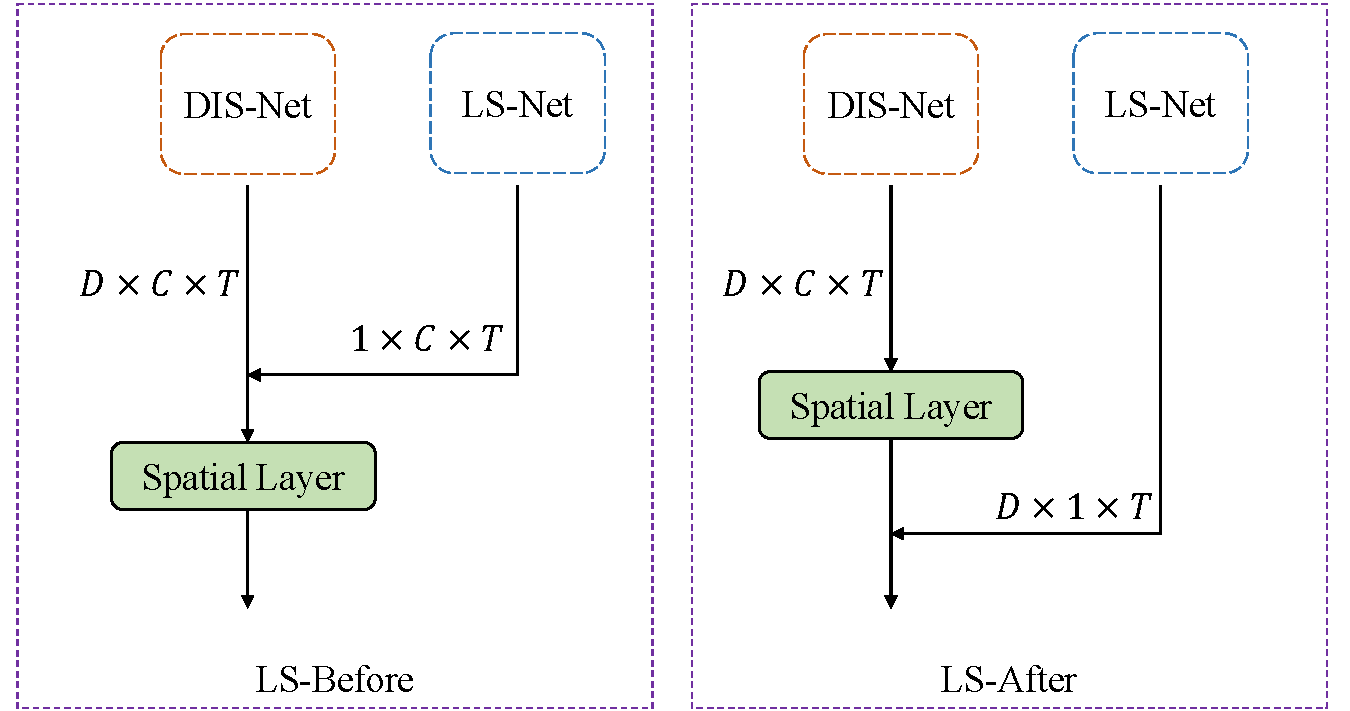
\includegraphics[width=0.6\textwidth]{fuse.pdf}
    \caption{不同融合方式}
    \label{fig:fuse}
\end{figure}

论文在2A数据集上使用HA-FuseNet进行实验,对这两种方式的效果予以验证。实验中对相关超参数进行了固定,从而只关注不同融合方式对性能造成的影响,表~\ref{tab:fuse}~对实验数据进行了展示,其中,准确率与Kappa系数为九位被试的平均表现。
\begin{table}[ht]
    \centering
    \caption{特征融合方式实验结果对比}
    \label{tab:fuse}
    \begin{tabularx}{\textwidth}{CCCC}
      \toprule
      Models & ACC(\%) & Kappa & SD \\
      \midrule
      LS-Before & \textbf{77.89} & \textbf{0.70} & \textbf{10.22} \\
      LS-After & 76.98 & 0.69 & 10.71 \\
      \bottomrule
    \end{tabularx}
\end{table}

数据显示,LS-Before具有更高的准确率和一致性,且不同被试的准确率差异较小,这可能是因为LS-Net主要进行了时序特征提取与全局时空自注意力加权两个操作,对空间维度的操作较缺乏,因此需要由空间卷积层进行空间维度的特征提取,以获得更丰富的特征表达;而LS-After将空间维度的特征视为深度维度,可能造成了特征之间的混淆,因此反而不利于提高分类的精确度。论文采用LS-Before的方式进行LS-Net和DIS-Net的特征融合。

\subsection{各模块消融实验}

为了探究论文所提出的各个模块的有效性,并研究不同模块对HA-FuseNet分类效果的影响,论文针对这些模块进行消融实验,按照模型构建的顺序,从基准模型开始,逐步对新增模块后的模型效果进行实验验证。

论文对不同结构的模型作以下定义:

(1) Inception:针对EEG信号的特点,修改了卷积核的基础Inception模型,具有三个Inception模块;

(2) Base-Inception:Inception+Bottleneck,即论文所提出的BaseNet。在Inception模型的基础上引入反转瓶颈层,并对分支数量、激活函数等进行了调整,同时,针对EEG信号的特性,对卷积核大小进行了调整;

(3) BI+Dense:Inception+Bottleneck+Dense Block,即论文所提出的DI-Net。在BaseNet的基础上,引入了密集连接模块;

(4) DI+svSE:Inception+Bottleneck+Dense Block+svSE,即论文所提出的DIS-Net。在DI-Net的基础上,引入了svSE混合注意力模块;

(5) DIS+LSTM:Inception+Bottleneck+Dense Block+svSE+LSTM。在DIS-Net的基础上,引入了LSTM网络;

(6) DIS+LSTM+SCoT:Inception+Bottleneck+Dense Block+svSE+LSTM+SCoT,即论文所提出的结合了DIS-Net和LS-Net的HA-FuseNet。在DIS+LSTM的基础上,引入了SCoT全局自注意力模块。

论文在2A数据集上进行消融实验,表~\ref{tab:ab}~展示了实验的结果,其中,准确率和Kappa系数是九位被试的平均结果。

\begin{table}[ht]
    \centering
    \caption{HA-FuseNet各模块消融实验结果对比}
    \label{tab:ab}
    \begin{tabularx}{\textwidth}{CCCC}
      \toprule
      Models & ACC(\%) & Kappa & SD \\
      \midrule
      Inception &67.40&0.56&16.15\\
      Base-Inception &72.35&0.63&12.27\\
      BI+Dense &74.42&0.65& 11.92\\
      DI+svSE &76.16&0.68&11.33\\
      DIS+LSTM &76.78 &0.69 & 10.72\\
      DIS+LSTM+SCoT &77.89&0.70&10.22 \\
      \bottomrule
    \end{tabularx}
\end{table}

实验数据显示,Inception+Bottleneck+Dense Block+svSE+LSTM+SCoT结构,即本文所提出的最终模型HA-FuseNet在MI-EEG分类任务上表现最好,准确率、Kappa一致性系数分别达到了77.89\%、0.70,标准差达到了10.22,证明在不同被试上,HA-FuseNet取得了最好的分类性能,且被试之间的准确率差异较小,具有较好的稳定性。

随着模型的逐渐复杂,准确率、Kappa一致性呈现上升趋势,标准差呈现下降趋势,证明了每个模块的有效性。此外,对Inception进行MI-EEG分类任务的针对性改进后得到的BaseNet具有最明显的提升,此后依次为多尺度密集连接模块、svSE模块、SCoT模块、LSTM模块。从对最终模型的贡献度来看,可能说明了相较于循环神经网络,卷积神经网络在MI-EEG分类任务上具有更大的优势。

实验证明了论文所提出的各个模块的有效性,这些模块共同构成了最终模型HA-FuseNet,在2A数据集上取得了77.89\%的平均准确率和0.70的平均Kappa一致性系数。在后续实验中,使用完整的模型。

\subsection{BCI Competition IV Dataset 2A数据集上的对比实验}

在相同的实验设置下,论文在BCI Competition IV Dataset 2A数据集上进行HA-FuseNet与主流模型的被试内(Subject Dependent)对比实验和被试间(Subject Independent)对比实验,以对HA-FuseNet相对于其他模型在MI-EEG分类任务中的性能进行评估。

论文所使用的与HA-FuseNet进行对比的模型中,ShallowConvNet\cite{schirrmeister2017deep}与DeepConvNet\cite{schirrmeister2017deep}是基于卷积神经网络搭建;EEGNet\cite{lawhern2018eegnet}参考了BCI领域经典算法FBCSP的思想,将深度可分离卷积引入了网络结构中;EEGResNet\cite{HBM:HBM23730}基于残差神经网络\cite{he2016deep}构建;EEGInception\cite{zhang2021eeg}使用了Inception多分支和残差连接;EEGConformer\cite{song2022eeg}使用Transformer\cite{vaswani2017attention}与卷积神经网络串联,用以EEG信号的解码;LMDA-Net\cite{miao2023lmda}提出了一种新颖的通道注意力模块和深度注意力模块,基于ShallowConvNet和EEGNet进行了改进。

对于BCI Competition IV Dataset 2A数据集,实验数据显示:

(1) HA-FuseNet在未进行数据增强的被试内实验中,取得了最优的准确率和Kappa一致性,且准确率标准差达到了10.22,证明了HA-FuseNet具有优秀的MI-EEG分类能力,且对不同的被试具有较好的稳定性;

(2) 使用SG轻量化卷积模块的HA-FuseNet(SG)在未进行数据增强的被试内实验中,尽管性能较HA-FuseNet有所下降,但准确率和Kappa系数仅次于ShallowConvNet,且标准差低于ShallowConvNet,HA-FuseNet(SG)的平均准确率较HA-FuseNet下降了约0.66个百分点,在一些被试上,其准确率高于HA-FuseNet;

(3) HA-FuseNet在被试间实验中,取得了最高的平均准确率和Kappa一致性,证明了HA-FuseNet具有优秀的跨被试泛化能力。

实验结果证实,论文所提出的模型HA-FuseNet具有一定的有效性,能够使用较小规模的数据集取得优秀的性能表现,且具有相较于基准模型最优的分类精度和跨被试泛化能力,而使用数据增强算法后,HA-FuseNet的性能表现能够得到进一步的增强。

\paragraph{被试内对比实验}

2A数据集共有九名被试,每名被试具有独立的训练集和测试集,被试内对比实验即使用每名被试对应的训练集和测试集,即为每名被试训练了一个模型。

表~\ref{tab:2acomparein}~展示了不同模型进行被试内实验的准确率,表~\ref{tab:2acompareinsd}~展示了被试内实验的Kappa一致性系数和标准差,其中,Kappa一致性系数为九名被试的平均值,标准差为准确率标准差。需要说明的是,表~\ref{tab:2acomparein}~和~\ref{tab:2acompareinsd}~展示的是未进行数据增强的结果,即对于每名被试,使用数据规模为288的训练集。为了更直观地对数据进行展示,在表~\ref{tab:2acomparein}~和表~\ref{tab:2acompareinsd}~中通过加粗的方式对基准模型中的最优值进行了强调。

\begin{table}[ht]
    \centering
    \caption{HA-FuseNet与基准模型在2A数据集上的被试内实验结果对比(Acc\%)}
    \label{tab:2acomparein}
    \begin{subtable}[ht]{\textwidth}
      \centering
    %   \caption{子表a}
      \label{tab:2acompareina}
      \begin{tabularx}{\textwidth}{cCCCCC}
        \toprule
        Models & 1 & 2 & 3 & 4 & 5\\
        \midrule
        ShallowConvNet\cite{schirrmeister2017deep}  & 84.03 & 61.46 & \textbf{94.10} & \textbf{70.83} & 73.26 \\
        DeepConvNet\cite{schirrmeister2017deep} & 83.68 & \textbf{65.28} & 90.63 & 69.44 & \textbf{76.04} \\
        EEGNet\cite{lawhern2018eegnet} & 78.13 & 63.54 & 82.30 & 60.42 & 71.88 \\
        EEGResNet\cite{HBM:HBM23730} & 69.10 & 40.97 & 63.89 & 49.65 & 45.49 \\
        EEGInception\cite{zhang2021eeg} & 71.18 & 48.26 & 82.29 & 55.90 & 64.58 \\
        EEGConformer\cite{song2022eeg} & 67.71 & 55.21 & 84.72 & 53.82 & 75.69 \\
        LMDA-Net\cite{miao2023lmda} & \textbf{86.46} & 60.46 & 90.97 & 59.02 & 69.10 \\
        \midrule 
        \textbf{HA-FuseNet}  & 87.67 & 62.85 & 92.36 & 67.54 & 75.00\\
        \textbf{HA-FuseNet(SG)} & 86.81 & 63.89 & 92.01 & 65.54 & 71.88\\
        \bottomrule
      \end{tabularx}
    \end{subtable}
    \begin{subtable}[ht]{\textwidth}
      \centering
    %   \caption{子表b}
      \label{tab:2acompareinb}
      \begin{tabularx}{\textwidth}{cCCCCCC}
        \toprule
        Models & 6 & 7 & 8 & 9 & Average \\
        \midrule
        ShallowConvNet\cite{schirrmeister2017deep}  & 55.90 & 85.76 & \textbf{89.24} & \textbf{85.42} & \textbf{77.78} \\
        DeepConvNet\cite{schirrmeister2017deep} & \textbf{64.58} & 89.93 & 79.51 & 73.61 & 76.97 \\
        EEGNet\cite{lawhern2018eegnet} & 59.03 & 72.92 & 68.06 & 66.67 & 69.21 \\
        EEGResNet\cite{HBM:HBM23730} & 42.36 & 54.51 & 61.11 & 64.93 & 54.67 \\
        EEGInception\cite{zhang2021eeg} & 52.43 & 75.00 & 85.41 & 73.61 & 67.63 \\
        EEGConformer\cite{song2022eeg} & 53.47 & 69.10 & 71.53 & 58.68 & 65.55 \\
        LMDA-Net\cite{miao2023lmda} & 55.90 & \textbf{90.28} & 81.94 & 76.04 & 74.50 \\
        \midrule 
        \textbf{HA-FuseNet}  & 65.97 & 89.58 & 81.60 & 78.47 & 77.89 \\
        \textbf{HA-FuseNet(SG)}  & 62.85 & 91.67 & 83.68 & 74.95 & 77.23 \\
        \bottomrule
      \end{tabularx}
    \end{subtable}
\end{table}
\begin{table}[H]
    \centering
    \caption{HA-FuseNet与基准模型在2A数据集上的被试内实验结果对比(Kappa/SD)}
    \label{tab:2acompareinsd}
    \begin{tabularx}{\textwidth}{CCC}
      \toprule
      Models & Kappa & SD \\
      \midrule
      ShallowConvNet\cite{schirrmeister2017deep} & \textbf{0.69} & 12.35\\
      DeepConvNet\cite{schirrmeister2017deep} & 0.69 & 9.22 \\
      EEGNet\cite{lawhern2018eegnet} & 0.60 & \textbf{7.40} \\
      EEGResNet\cite{HBM:HBM23730} & 0.36 & 9.94 \\
      EEGInception\cite{zhang2021eeg} & 0.56 & 12.41 \\
      EEGConformer\cite{song2022eeg} & 0.53 & 10.33 \\
      LMDA-Net\cite{miao2023lmda} & 0.65 & 13.01 \\
      \midrule 
      \textbf{HA-FuseNet} &0.70&10.22\\
      \textbf{HA-FuseNet(SG)} &0.69&11.14\\
      \bottomrule
    \end{tabularx}
\end{table}

对比基准模型的实验数据,可以发现以下结果:

(1) 对于基准模型,ShallowConvNet取得了最高的平均准确率与Kappa值,但准确率标准差达到了12.35,表明不同被试之间的准确率差异较为明显,性能相对不均衡;

(2) EEGNet取得了最优的准确率标准差,表明不同被试之间准确率差异较小,性能比较均衡,但平均准确率与Kappa值分别为69.21\%、0.60,低于ShallowConvNet、DeepConvNet和LMDA-Net;

(3) LMDA-Net的平均准确率与Kappa值仅低于ShallowConvNet、DeepConvNet,但取得了最高的准确率标准差,表明不同被试之间准确率差异最为明显,由于LMDA-Net是基于EEGNet和ShallowConvNet的改进,这种差异主要可能来源于LMDA-Net提出的局部通道注意力与深度注意力机制,对不同被试特征的关注能力较为不均衡;

(4) EEGResNet取得了最差的效果,低于EEGConformer,这可能是因为在未进行数据增强的情况下,EEGResNet无法很好地发挥其深度架构的优势,而EEGConformer使用了未经过预训练的Transformer,这可能成为其在较小规模的数据集上表现不优的原因;

对比基准模型和论文提出的模型的实验数据,可以发现HA-FuseNet取得了最高的平均准确率和Kappa值,且在1号被试和6号被试上取得了最高的准确率,对于其他模型平均表现较差的2号和4号被试,HA-FuseNet也取得了良好的性能。同时,HA-FuseNet的准确率标准差低于具有次优平均准确率和Kappa值的ShallowConvNet;使用SG轻量化卷积模块的HA-FuseNet(SG)取得了仅次于ShallowConvNet的准确率和Kappa一致性,其准确率的标准差同样低于ShallowConvNet。相较于HA-FuseNet,HA-FuseNet(SG)的平均准确率仅下降了约0.66个百分点。

实验证明了HA-FuseNet和HA-FuseNet(SG)的有效性,能够在使用小规模数据集的情况下取得较好的性能表现。此外,通过对各项模型的实验结果分析,印证了先前研究中,关于浅层网络在小规模数据集的MI-EEG分类任务中性能表现优良的理论,而多尺度密集连接使得HA-FuseNet能够同时利用多尺度的低级特征和高级语义信息,同时,通过全局自注意力机制和局部混合注意力机制进行多维的加权,利用LSTM对时间维度的长短期依赖关系进行提取,综合取得了较基准模型更好的性能。

\paragraph{数据增强被试内对比实验}

论文采用数据增强算法对训练集进行扩充,并扩充至原本的四倍(其中包括原始数据)。需要说明的是,进行数据增强算法延长了模型的训练时间,增大了计算消耗。

表~\ref{tab:2acompareag}~展示了进行数据增强后各模型在2A数据集上进行被试内实验的准确率,表~\ref{tab:2acompareagsd}~则展示了Kappa系数和标准差的对比结果。为了展示的直观性,同样对基准网络中的最优值进行了加粗展示。

数据显示,除EEGConformer之外,其他模型的平均准确率均有所上升,其中,EEGInception的平均准确率升高了10.79个百分点,EEGResNet升高了约9.9个百分点,DeepConvNet和HA-FuseNet的平均准确率上升幅度则相对较小,但论文研究的重点在于基于小规模数据集的MI-EEG分类,因此并无太大影响。这证明了数据增强算法的有效性,可以基于此增加模型学习不同频带数据分布的能力,从而提升模型的性能表现。

\begin{table}[ht]
    \centering
    \caption{基于数据增强的HA-FuseNet与基准模型在2A数据集上的被试内实验结果对比(Acc\%)}
    \label{tab:2acompareag}
    \begin{subtable}[ht]{\textwidth}
      \centering
    %   \caption{子表a}
      \label{tab:2acompareaga}
      \begin{tabularx}{\textwidth}{CCCCCC}
        \toprule
        Models & 1 & 2 & 3 & 4 & 5\\
        \midrule
        ShallowConvNet\cite{schirrmeister2017deep}  & \textbf{89.72} & 66.20 & 94.34 & \textbf{84.54} & \textbf{76.39} \\
        DeepConvNet\cite{schirrmeister2017deep} & 82.58 & 62.37 & 91.11 & 73.14 & 69.18 \\
        EEGNet\cite{lawhern2018eegnet} & 77.61 & 67.77 & \textbf{94.95} & 66.25 & 61.63 \\
        EEGResNet\cite{HBM:HBM23730} & 77.88 & 53.05 & 76.22 & 65.37 & 49.39 \\
        EEGInception\cite{zhang2021eeg}  & 88.07 & 61.93 & 91.29 & 77.83 & 69.97 \\
        EEGConformer\cite{song2022eeg}  & 80.05 & 47.82 & 85.98 & 25.27 & 58.25 \\
        LMDA-Net\cite{miao2023lmda} & 88.15 & \textbf{69.16} & 91.99 & 81.18 & 70.31 \\
        \midrule 
        \textbf{HA-FuseNet} & 90.37 & 67.85 & 94.36 & 72.14 & 77.08\\
        \bottomrule
      \end{tabularx}
    \end{subtable}
    \begin{subtable}[ht]{\textwidth}
      \centering
    %   \caption{子表b}
      \label{tab:2acompareagb}
      \begin{tabularx}{\textwidth}{CCCCCCC}
        \toprule
        Models & 6 & 7 & 8 & 9 & Average \\
        \midrule
        ShallowConvNet\cite{schirrmeister2017deep}  & \textbf{62.24} & \textbf{96.69} & \textbf{90.94} & \textbf{89.55} & \textbf{83.40} \\
        DeepConvNet\cite{schirrmeister2017deep}  & 59.38 & 86.85 & 85.80 & 82.58 & 77.00 \\
        EEGNet\cite{lawhern2018eegnet} & 46.09 & 85.80 & 83.71 & 87.63 & 74.61 \\
        EEGResNet\cite{HBM:HBM23730}  & 44.44 & 77.61 & 75.35 & 61.85 & 64.57 \\
        EEGInception\cite{zhang2021eeg} & 57.03 & 90.33 & 84.76 & 84.58 & 78.42 \\
        EEGConformer\cite{song2022eeg}  & 26.65 & 52.27 & 27.00 & 25.61 & 47.65 \\
        LMDA-Net\cite{miao2023lmda}& 60.24 & 93.21 & 83.28 & 86.41 & 80.44 \\
        \midrule 
        \textbf{HA-FuseNet} & 67.92 & 93.75 & 83.68 & 87.15 & 81.56 \\
        \bottomrule
      \end{tabularx}
    \end{subtable}
\end{table}
\begin{table}[H]
    \centering
    \caption{基于数据增强的HA-FuseNet与基准模型在2A数据集上的被试内实验结果对比(Kappa/SD)}
    \label{tab:2acompareagsd}
    \begin{tabularx}{\textwidth}{CCC}
      \toprule
      Models & Kappa & SD \\
      \midrule
      ShallowConvNet\cite{schirrmeister2017deep} & \textbf{0.78} & 11.67 \\
      DeepConvNet\cite{schirrmeister2017deep} & 0.69 & \textbf{10.73} \\
      EEGNet\cite{lawhern2018eegnet} & 0.66 & 14.52 \\
      EEGResNet\cite{HBM:HBM23730} & 0.53 & 12.36 \\
      EEGInception\cite{zhang2021eeg} & 0.71 & 11.92 \\
      EEGConformer\cite{song2022eeg} & 0.30 & 22.38 \\
      LMDA-Net\cite{miao2023lmda} & 0.74 & 10.74 \\
      \midrule 
      \textbf{HA-FuseNet} & 0.76 & 10.09 \\
      \bottomrule
    \end{tabularx}
\end{table}

值得注意的是,EEGConformer的性能反而出现了下降,这说明基于频率混叠的数据增强算法或许并不适用于Transformer架构,这可能说明了EEGConformer将Transformer直接引入卷积层之后形成串联模型的方式具有受限的提取不同频率成分的能力。如果要将Transformer应用于MI-EEG分类任务中,采用合适的滤波器进行数据预处理,并基于其他方法进行数据增强从而形成较大规模的数据集,可能是更适合的方法,例如,在EEGConformer论文中,使用了基于滑动窗口的数据增强方法\cite{song2022eeg}。

此外,表~\ref{tab:2acompareagsd}~表明进行数据增强之后,除EEGConformer之外,其他模型的Kappa一致性均有所上升。论文所提出的HA-FuseNet的Kappa值达到了0.76,准确率的标准差下降为10.09,为所有模型中的最低值,表明HA-FuseNet的在不同被试间的稳定性得到了进一步的加强。

\paragraph{被试间对比实验}

在被试间对比实验中,对于被试\(i\),使用全部其他被试的训练集为被试\(i\)的训练集,如公式~\ref{eq:cross}~所示,其中,\(Train_j\)表示被试\(j\)的训练集。仍然使用被试\(i\)的测试集为测试集。
\begin{equation}
    \label{eq:cross}
    Train_i=\sum_{j}^{N}Train_j,\,i \in [1,9],\,j \in [1,9],\,j \neq i
\end{equation}

表~\ref{tab:2acomparecross}~展示了各个模型进行被试间实验的准确率结果对比,例如,表格中[ShallowConvNet,1]即表示ShallowConvNet使用其他八名被试的训练集集合,在1号被试的测试集上得到的准确率。表~\ref{tab:2acomparecrosssd}~展示了被试间实验的Kappa系数和标准差结果对比,其中,Kappa系数为九名被试的平均值。被试间对比实验未使用数据增强算法。

在表~\ref{tab:2acomparecross}~和表~\ref{tab:2acomparecrosssd}~,同样采用了加粗的方式对基准模型中的最优值进行了展示。

对比基准模型的实验数据,可以发现以下结果:

(1) DeepConvNet在基准模型中具有最高的平均准确率和Kappa系数,准确率标准差达到了9.54,DeepConvNet在被试间实验中取得了优于ShallowConvNet的性能,这可能是因为DeepConvNet学习到了更为抽象和高级的特征,从而更好地适应了不同被试间的数据差异;

(2) EEGNet取得了最优的准确率标准差,但平均准确率和Kappa值为63.23\%、0.51,仅优于EEGResNet和EEGConformer,这说明了EEGNet具有较好的稳定性,但分类的准确率和一致性较差;

(3) 所有基准模型在被试2号、4号、6号的跨被试实验中,平均性能表现较差。

对比基准模型和论文提出的模型的实验数据,可以发现论文提出的HA-FuseNet取得了最优的平均准确率和Kappa系数,且平均准确率比DeepConvNet提升了约0.63\%,HA-FuseNet的准确率标准差达到了11.06,仅比DeepConvNet上升了约0.52。

此外,论文提出的HA-FuseNet在被试1/2/3/7/8/9号上的表现优于DeepConvNet,仅在被试4/5/6号上的表现低于DeepConvNet。但应当注意到,在基准模型平均性能较差的被试2/4/6号上,HA-FuseNet取得了较为均衡的分类精度,在被试2号中,HA-FuseNet的精度仅低于EEGNet,被试4号中,仅低于DeepConvNet和EEGNet。

实验证实了论文提出的HA-FuseNet在具有22通道的2A数据集上具有良好的分类性能和跨被试泛化能力,能够满足论文的研究目标。

\begin{table}[H]
    \centering
    \caption{HA-FuseNet与基准模型在2A数据集上的被试间实验结果对比(Acc\%)}
    \label{tab:2acomparecross}
    \begin{subtable}[ht]{\textwidth}
      \centering
    %   \caption{子表a}
      \label{tab:2acomparecrossa}
      \begin{tabularx}{\textwidth}{CCCCCC}
        \toprule
        Models & 1 & 2 & 3 & 4 & 5\\
        \midrule
        ShallowConvNet\cite{schirrmeister2017deep}   & \textbf{76.39} & 47.92 & \textbf{88.54} & 55.56 & 57.64\\
        DeepConvNet\cite{schirrmeister2017deep} & 71.53 & 50.69 & 84.72 & \textbf{61.46} & \textbf{69.10} \\
        EEGNet\cite{lawhern2018eegnet} & 68.75 & \textbf{56.60} & 68.75 & 61.11 & 68.75 \\
        EEGResNet\cite{HBM:HBM23730} & 61.81 & 38.54 & 64.24 & 45.83 & 39.93 \\
        EEGInception\cite{zhang2021eeg}  & 74.31 & 51.04 & 81.60 & 52.43 & 56.25 \\
        EEGConformer\cite{song2022eeg}  & 52.78 & 26.04 & 26.04 & 50.00 & 64.24\\
        LMDA-Net\cite{miao2023lmda} & 72.22 & 47.22 & 83.68 & 55.90 & 51.74 \\
        \midrule 
        \textbf{HA-FuseNet}  & 76.13 & 52.79 & 86.89 & 57.13 & 60.42\\
        \bottomrule
      \end{tabularx}
    \end{subtable}
    \begin{subtable}[ht]{\textwidth}
      \centering
    %   \caption{子表b}
      \label{tab:2acomparecrossb}
      \begin{tabularx}{\textwidth}{CCCCCCC}
        \toprule
        Models & 6 & 7 & 8 & 9 & Average \\
        \midrule
        ShallowConvNet\cite{schirrmeister2017deep}  & 55.21 & 74.65 & \textbf{81.25} & 72.92 & 67.79 \\
        DeepConvNet\cite{schirrmeister2017deep}  & 59.03 & \textbf{75.35} & 74.31 & 64.93 & \textbf{67.90} \\
        EEGNet\cite{lawhern2018eegnet}  & 58.68 & 73.61 & 56.60 & 56.25 & 63.23 \\
        EEGResNet\cite{HBM:HBM23730}  & 42.01 & 47.22 & 50.69 & 56.25 & 49.61 \\
        EEGInception\cite{zhang2021eeg}  & \textbf{60.42} & 71.18 & 73.96 & \textbf{74.31} & 66.17 \\
        EEGConformer\cite{song2022eeg} & 25.00 & 26.74 & 29.51 & 27.78 & 36.46\\
        LMDA-Net\cite{miao2023lmda}  & 48.26 & 71.88 & 76.04 & 66.67 & 63.73\\
        \midrule 
        \textbf{HA-FuseNet}  & 58.49 & 76.74 & 78.13 & 70.06 & 68.53 \\
        \bottomrule
      \end{tabularx}
    \end{subtable}
\end{table}
\begin{table}[ht]
    \centering
    \caption{HA-FuseNet与基准模型在2A数据集上的被试间实验结果对比(Kappa/SD)}
    \label{tab:2acomparecrosssd}
    \begin{tabularx}{\textwidth}{CCC}
      \toprule
      Models & Kappa & SD \\
      \midrule
      ShallowConvNet\cite{schirrmeister2017deep} &0.57&13.19 \\
      DeepConvNet\cite{schirrmeister2017deep} &\textbf{0.57} &9.54\\
      EEGNet\cite{lawhern2018eegnet} &0.51& \textbf{6.33}\\
      EEGResNet\cite{HBM:HBM23730} &0.33&8.83\\
      EEGInception\cite{zhang2021eeg} &0.55&10.57\\
      EEGConformer\cite{song2022eeg}&0.15&14.09 \\
      LMDA-Net\cite{miao2023lmda} &0.52&12.53\\
      \midrule 
      \textbf{HA-FuseNet} &0.57&11.06\\
      \bottomrule
    \end{tabularx}
\end{table}

\subsection{BCI Competition IV Dataset 2B数据集上的对比实验}

为了评估论文所提出的模型在不同硬件设施(电极数量)的场景下的性能,论文在BCI Competition IV Dataset 2B数据集上进行HA-FuseNet与主流模型的被试内和被试间对比实验。相较于2A数据集的22通道,2B数据集仅使用3个通道记录EEG数据,对模型在较低空间分辨率条件下的性能提出了挑战。2B数据集上的实验未进行数据增强,以对模型在小规模数据集上的表现进行评估。

论文所使用的与HA-FuseNet进行对比的基准模型与前文相同,包括ShallowConvNet\cite{schirrmeister2017deep}、DeepConvNet\cite{schirrmeister2017deep}、EEGNet\cite{lawhern2018eegnet}、EEGResNet\cite{HBM:HBM23730}、EEGInception\cite{zhang2021eeg}、EEGConformer\cite{song2022eeg}和LMDA-Net\cite{miao2023lmda}。

对于BCI Competition IV Dataset 2B数据集,实验数据显示HA-FuseNet在被试内实验和被试间实验中,均取得了最优的平均准确率和Kappa一致性。在被试内实验中,HA-FuseNet的平均准确率、Kappa系数和准确率标准差分别达到了75.23\%、0.50和8.84,其中,准确率标准差仅高于具有较差性能表现的EEGResNet。在被试间实验中,HA-FuseNet的平均准确率、Kappa系数和准确率标准差分别达到了76.86\%、0.53和6.68,其中,准确率标准差仅高于性能表现最差的EEGConformer。

实验结果证明了论文所提出的HA-FuseNet具有良好的适应低空间分辨率场景的能力,其具有优秀的分类精度和分类一致性,在不同被试上具有稳定的泛化能力,同时,HA-FuseNet对数据增强算法没有强依赖性,在小规模数据集上也表现出优秀的性能。

\paragraph{被试内对比实验}

2B数据集共有九名被试,被试内对比实验即对每名被试,使用其训练集和测试集数据进行独立的训练和测试。

表~\ref{tab:2bcomparein}~展示了HA-FuseNet和基准模型进行被试内实验的准确率,其中,最后一列为九名被试的平均准确率。表~\ref{tab:2bcompareinsd}~展示了各个模型进行被试内实验的Kappa一致性系数和准确率的标准差,其中,Kappa一致性系数为九名被试的均值。在表~\ref{tab:2bcomparein}~和表~\ref{tab:2bcompareinsd}~中,通过加粗的方式标明了基准模型取得的最优数据。

对比基准模型的实验数据,可以发现以下结果:

(1) EEGInception在基准模型中具有最高的平均准确率和Kappa系数,其表现超过了ShallowConvNet,后者在2A数据集上具有最优的准确率和一致性表现。这说明了EEGInception具有更好的适应低空间分辨率场景的能力,而ShallowConvNet的适应性则有所下降,这种差异可能来源于二者的架构差别,EEGInception着重提取时间维度特征,而ShallowConvNet对时域和空域的特征应用了相同的策略;

(2) EEGResNet取得了最优的准确率标准差,表明在不同被试之间的性能较为稳定,然而,EEGResNet的平均准确率为68.51\%,相较于EEGInception降低了6.07个百分点,说明其分类精度相对较差;

\begin{table}[ht]
    \centering
    \caption{HA-FuseNet与基准模型在2B数据集上的被试内实验结果对比(Acc\%)}
    \label{tab:2bcomparein}
    \begin{subtable}[ht]{\textwidth}
      \centering
    %   \caption{子表a}
      \label{tab:2bcompareina}
      \begin{tabularx}{\textwidth}{CCCCCC}
        \toprule
        Models & 1 & 2 & 3 & 4 & 5\\
        \midrule
        ShallowConvNet\cite{schirrmeister2017deep}  & 78.33 & 74.17 & 59.17 & 90.77 & 63.08\\
        DeepConvNet\cite{schirrmeister2017deep}  & 78.33 & 72.50 & 59.17 & \textbf{97.69} & 68.46\\
        EEGNet\cite{lawhern2018eegnet}  & 78.33 & 73.33 & 60.00 & 94.61 & 59.23 \\
        EEGResNet\cite{HBM:HBM23730}  & 68.33 & 62.50 & 58.33 & 87.69 & 70.00 \\
        EEGInception\cite{zhang2021eeg}  & \textbf{81.67} & 70.83 & 63.33 & 90.00 & \textbf{82.31} \\
        EEGConformer\cite{song2022eeg}  & 72.50 & 73.33 & 60.00 & 88.46 & 56.92\\
        LMDA-Net\cite{miao2023lmda}  & 76.67 & \textbf{75.00} & \textbf{65.00} & 93.85 & 64.61 \\
        \midrule 
        \textbf{HA-FuseNet}   & 79.17 & 80.00 & 70.83 & 95.39 & 76.92 \\
        \bottomrule
      \end{tabularx}
    \end{subtable}
    \begin{subtable}[ht]{\textwidth}
      \centering
    %   \caption{子表b}
      \label{tab:2bcompareinb}
      \begin{tabularx}{\textwidth}{CCCCCCC}
        \toprule
        Models & 6 & 7 & 8 & 9 & Average \\
        \midrule
        ShallowConvNet\cite{schirrmeister2017deep}  & 80.83 & 68.33 & 59.29 & 60.83 & 70.53 \\
        DeepConvNet\cite{schirrmeister2017deep}  & 80.00 & \textbf{76.67} & 63.57 & 60.00 & 72.93 \\
        EEGNet\cite{lawhern2018eegnet}  & 66.67 & 72.50 & 57.86 & 57.50 & 68.89 \\
        EEGResNet\cite{HBM:HBM23730}  & 73.33 & 67.50 & \textbf{66.43} & 62.50 & 68.51\\
        EEGInception\cite{zhang2021eeg}  & \textbf{81.67} & 69.17 & \textbf{66.43} & \textbf{65.83} & \textbf{74.58} \\
        EEGConformer\cite{song2022eeg}  & 70.83 & 70.83 & 60.71 & 60.83 & 68.27\\
        LMDA-Net\cite{miao2023lmda}  & 80.00 & 70.83 & 60.71 & 56.67 & 71.48 \\
        \midrule 
        \textbf{HA-FuseNet}   & 75.00 & 69.17 & 66.43 & 64.17 & 75.23 \\
        \bottomrule
      \end{tabularx}
    \end{subtable}
\end{table}
\begin{table}[H]
    \centering
    \caption{HA-FuseNet与基准模型在2B数据集上的被试内实验结果对比(Kappa/SD)}
    \label{tab:2bcompareinsd}
    \begin{tabularx}{\textwidth}{CCC}
      \toprule
      Models & Kappa & SD \\
      \midrule
      ShallowConvNet\cite{schirrmeister2017deep} &0.41&10.54\\
      DeepConvNet\cite{schirrmeister2017deep} &0.45&11.40\\
      EEGNet\cite{lawhern2018eegnet} &0.38& 11.61\\
      EEGResNet\cite{HBM:HBM23730} &0.37&\textbf{7.99}\\
      EEGInception\cite{zhang2021eeg} &\textbf{0.49}&8.89\\
      EEGConformer\cite{song2022eeg} &0.36&9.27\\
      LMDA-Net\cite{miao2023lmda} &0.43&10.73\\
      \midrule 
      HA-FuseNet &0.50&8.84\\
      \bottomrule
    \end{tabularx}
\end{table}

(3) 2A数据集上,各个基准模型取得的平均准确率的均值约为69.47\%,高于平均值的模型有ShallowConvNet、DeepConvNet和LMDA-Net;2B数据集上,各个基准模型取得的平均准确率的均值约为70.74\%,高于平均值的模型有DeepConvNet、EEGInception和LMDA-Net;此外,相较于2A数据集,EEGResNet、EEGConformer在2B数据集上的准确率更接近均值,EEGNet落后均值的幅度增加,DeepConvNet、LMDA-Net领先均值的幅度则降低了。这或许说明了空间分辨率较高时,EEG信号特征明显,因此浅层网络就能够取得较好的效果,而空间分辨率较低时,需要更为复杂的网络提取EEG信号的特征。此外,LMDA-Net证明了针对EEG信号特性设计的注意力模块能够取得良好的效果。

基准模型的实验结果印证了论文设计模型的思路的正确性,包括更关注时间维度特征、同时利用深层和浅层特征、针对EEG信号特性设计注意力模块等。这些设计使得HA-FuseNet对空间分辨率具有低依赖性,即对于高空间分辨率和低空间分辨率的场景,都能取得较好的性能表现。

实验数据证实,相较于基准模型,HA-FuseNet取得了最高的平均准确率和Kappa值,分别达到了75.23\%和0.50,在被试2/3/8号上取得了所有模型中最优的准确率,且在被试4/7号上取得了高于或持平于次优模型EEGInception的准确率。HA-FuseNet的准确率标准差达到了8.84,优于EEGInception,仅次于EEGResNet,证明HA-FuseNet不仅具有优秀的分类精度,同时在不同被试间具有良好的稳定性。

\paragraph{被试间对比实验}

被试间对比实验中,对于一名被试,使用其他所有被试的训练集为该被试的训练集,即训练集的数据规模为\(120\times8\),测试集为该被试的测试集,数据规模仍然为120。

表~\ref{tab:2bcomparecross}~展示了2B数据集上HA-FuseNet和基准模型进行被试间实验的准确率,其中,最后一列为九名被试的平均准确率。表~\ref{tab:2bcomparecrosssd}~展示了被试间实验的Kappa一致性系数和准确率标准差,其中,Kappa系数为九名被试的平均值。表~\ref{tab:2bcomparecross}~和表~\ref{tab:2bcomparecrosssd}~中对基准模型中的最优值进行了加粗展示。

对比基准模型的实验数据,可以发现以下结果:

(1) EEGInception在基准模型之中具有最优的准确率和Kappa系数,准确率平均值达到了75.64\%,高于次优模型ShallowConvNet大约0.12个百分点;EEGInception的准确率标准差为7.29,约比ShallowConvNet高0.11。这说明EEGInception的分类精度高于ShallowConvNet,但稳定性相对较差。相较于被试内实验,ShallowConvNet在被试间实验中的性能获得了明显的提升,其原因可能是较大的数据规模、较多变的数据分布弥补了ShallowConvNet学习低空间分辨率场景特征能力的不足,相当于ShallowConvNet经过了基于样本集合的数据增强。尽管如此,EEGInception仍然取得了最高的分类精度;

(2) EEGConformer取得了最低的准确率标准差,为6.44,但EEGConformer的平均准确率为基准模型中的最低值,因此,虽然EEGConformer在不同被试之间的稳定性相对较优,但较低的分类精度表明其综合性能仍然较差。

\begin{table}[h]
    \centering
    \caption{HA-FuseNet与基准模型在2B数据集上的被试间实验结果对比(Acc\%)}
    \label{tab:2bcomparecross}
    \begin{subtable}[ht]{\textwidth}
      \centering
    %   \caption{子表a}
      \label{tab:2bcomparecrossa}
      \begin{tabularx}{\textwidth}{CCCCCC}
        \toprule
        Models & 1 & 2 & 3 & 4 & 5\\
        \midrule
        ShallowConvNet\cite{schirrmeister2017deep}  & 75.00 & 67.50 & 70.83 & \textbf{92.20} & 76.46\\
        DeepConvNet\cite{schirrmeister2017deep}  & 67.50 & 65.00 & 67.50 & 91.54 & 72.31 \\
        EEGNet\cite{lawhern2018eegnet}  & 63.33 & \textbf{70.83} & \textbf{73.33} & 85.39 & 73.85 \\
        EEGResNet\cite{HBM:HBM23730}  & 62.50 & 67.50 & 62.50 & 89.23 & 72.31\\
        EEGInception\cite{zhang2021eeg} & \textbf{77.50} & 63.33 & 72.50 & 87.69 & \textbf{80.00} \\
        EEGConformer\cite{song2022eeg}  & 58.33 & 67.50 & 65.83 & 63.85 & 70.00 \\
        LMDA-Net\cite{miao2023lmda}  & 70.00 & 67.50 & 72.50 & 90.77 & 72.31 \\
        \midrule 
        \textbf{HA-FuseNet}  & 70.80 & 67.50 & 89.23 & 75.39 & 82.50 \\
        \bottomrule
      \end{tabularx}
    \end{subtable}
    \begin{subtable}[ht]{\textwidth}
      \centering
    %   \caption{子表b}
      \label{tab:2bcomparecrossb}
      \begin{tabularx}{\textwidth}{CCCCCCC}
        \toprule
        Models & 6 & 7 & 8 & 9 & Average \\
        \midrule
        ShallowConvNet\cite{schirrmeister2017deep}  & 81.67 & 75.83 & \textbf{70.14} & 70.00 & 75.52 \\
        DeepConvNet\cite{schirrmeister2017deep}  & 86.67 & 76.67 & 70.00 & \textbf{70.83} & 74.22 \\
        EEGNet\cite{lawhern2018eegnet}  & 82.50 & \textbf{85.00} & 70.00 & 69.17 & 74.82 \\
        EEGResNet\cite{HBM:HBM23730}  & 78.33 & 69.17 & 69.29 & 65.00 & 70.65 \\
        EEGInception\cite{zhang2021eeg}  & \textbf{85.00} & 74.17 & 71.43 & 69.17 & \textbf{75.64} \\
        EEGConformer\cite{song2022eeg}  & 78.33 & 78.33 & 67.86 & 61.67 & 67.97 \\
        LMDA-Net\cite{miao2023lmda}  & 84.17 & 79.17 & 70.71 & 69.17 & 75.14 \\
        \midrule 
        \textbf{HA-FuseNet}  & 82.50 & 80.00 & 72.14 & 71.67 & 76.86\\
        \bottomrule
      \end{tabularx}
    \end{subtable}
\end{table}

\begin{table}[H]
    \centering
    \caption{HA-FuseNet与基准模型在2B数据集上的被试间实验结果对比(Kappa/SD)}
    \label{tab:2bcomparecrosssd}
    \begin{tabularx}{\textwidth}{CCC}
      \toprule
      Models & Kappa & SD \\
      \midrule
      ShallowConvNet\cite{schirrmeister2017deep} &0.52&7.18\\
      DeepConvNet\cite{schirrmeister2017deep} &0.49& 8.62 \\
      EEGNet\cite{lawhern2018eegnet} &0.51& 7.31\\
      EEGResNet\cite{HBM:HBM23730} &0.39 &8.07\\
      EEGInception\cite{zhang2021eeg} & \textbf{0.52} &7.29 \\
      EEGConformer\cite{song2022eeg} &0.35 &\textbf{6.44}\\
      LMDA-Net\cite{miao2023lmda} &0.52&7.43\\
      \midrule 
      \textbf{HA-FuseNet} &0.53&6.68\\
      \bottomrule
    \end{tabularx}
\end{table}

实验数据显示,论文提出的HA-FuseNet的平均准确率和Kappa系数均优于基准模型,分别为76.86\%和0.53,其准确率标准差为6.68,仅高于EEGConformer。然而,考虑到EEGConformer较差的分类精度,仍然可以认为HA-FuseNet的综合性能超过了所有的基准模型。这与在2A数据集上的实验结论相符,HA-FuseNet具有优秀的分类精度和跨被试泛化性能力,且可以使用小规模数据集进行训练,同时,在不同精度的空间分辨率条件下都具有较为稳定的性能。实验证明了HA-FuseNet的有效性。

\section{本章小结}

本章主要对于第三章构建的MI-EEG分类网络HA-FuseNet进行了消融实验、对比实验和跨被试泛化性实验。首先,介绍了实验使用的软硬件环境。其次,介绍了实验所使用的数据集以及对数据进行处理的方法,同时介绍了实验中所使用的基本配置,包括超参数、损失函数、评估指标等。实验使用BCI Competition IV Dataset 2A数据集和2B数据集,其具有不同的通道数,能够对模型在不同空间分辨率下的性能进行评估。最后,介绍了具体进行的实验:首先,设计并进行实验,验证不同的网络结构对HA-FuseNet性能的影响,从而选择最合适的架构方式;其次,通过在不同数据集上,与当前的多种主流MI-EEG分类模型进行被试内对比实验、被试间对比实验,评估HA-FuseNet的分类精度、被试间稳定性、跨被试泛化性、跨空间分辨率泛化性能力。实验结果证明,HA-FuseNet相较于基准模型取得了综合最优的各项性能,从而证明了论文所提出方法的有效性。
% chapter5 总结

\chapter{总结与展望}

\section{总结}

随着各国脑科学计划的推进和脑机接口技术的不断发展,运动想象分类领域逐渐吸引了研究者们越来越多的注意,然而,现有的方法仍然存在对数据增强算法和神经科学先验知识具有依赖性,跨被试和不同空间分辨率场景的稳定性较差等问题,需要进一步对方法的通用性、稳定性和简便性进行增强。因此,论文基于特征融合与注意力机制构建了一种端到端的运动想象脑电图分类网络HA-FuseNet,并通过一系列实验证明了其具有利用小规模数据集达到较好的分类精度的能力,同时,在低空间分辨率与跨被试场景中,HA-FuseNet同样具有良好的稳定性,从而验证了模型的有效性。

现将论文的主要研究成果总结如下:

(1) 针对EEG信号特征相对简单,深层语义信息与浅层特征同等重要的特点,构建了多尺度密集连接模块(Dense Inception Module),以提取更为丰富和完整的EEG信号特征。通过反转瓶颈层,促进二维EEG信号的时空特征融合;根据EEG信号的采样频率设计卷积核的大小,以提取对应尺度的时间/频率特征;通过在多个分支应用多个不同尺度的卷积核,扩大特征提取的广度;通过密集连接方式对浅层特征和深层特征加以融合,获取更全面的特征表达;采取集中关注时间维度特征的策略,使用轴向的时间卷积核和空间卷积核,并堆叠相对更深的时间卷积层,以增强模型对不同精度的空间分辨率的适应性;

(2) 针对EEG信号非平稳、信噪比低、冗余信息较多的特点,构建了svSE混合注意力模块,以增强模型对重点数据的关注度。针对MI-EEG信号随时间变化波动明显,呈现出最大类内方差的特点\cite{mane2021fbcnet},svSE模块提出一种方差池化的方法,与平均池化相结合,以均衡且有针对性地对MI-EEG信号特征进行表征;针对EEG信号二维数据时空相关性不强的特点,svSE模块使用轴向注意力机制分别对时空维度进行建模,以适应不同形式的数据分布;

(3) 针对卷积神经网络无法获取全局依赖信息的问题,将LSTM与全局自注意力SCoT模块进行结合(LS-Net),以对EEG信号的长期依赖关系进行建模。SCoT模块采用两阶段计算的方式,首先计算空间域的全局自注意力并对原始数据进行加权,其次计算时空域的全局自注意力,对数据进行二次加权,以获得更全面的校准后的自注意力权重;通过全局依赖信息与局部依赖信息在深度维度的聚合,以在不形成干扰的情况下对局部与全局特征进行利用;

(4) 针对MI-EEG数据规模小,现有方法参数规模大、计算开销高、容易过拟合的问题,对论文所提出的模型HA-FuseNet进行了轻量化,以对小规模数据集进行适应,减少计算开销。HA-FuseNet通过轴向可分离卷积、深度可分离卷积削减参数规模,并提出了SG轻量化卷积模块,将参数规模与FLOPs分别缩减了约75\%和80\%;

(5) 在不同数据集上进行了一系列实验,对论文所提出的HA-FuseNet与多项基准模型的性能进行评估,并对实验结果展开了一系列讨论。在具有22通道的BCI Competition IV Dataset 2A数据集上,被试内实验中,HA-FuseNet的平均准确率和Kappa系数较次优模型ShallowConvNet分别提升了约0.11\%和0.01,准确率标准差优化了约1.21;被试间实验中,平均准确率和准确率标准差分别较次优模型DeepConvNet优化了约0.74\%和2.13。在具有3通道的BCI Competition IV Dataset 2B数据集上,被试内实验中,HA-FuseNet的平均准确率和Kappa系数较次优模型EEGInception分别提升了约0.65\%和0.01,准确率标准差优化了约0.05;被试间实验中,HA-FuseNet的平均准确率、Kappa系数和准确率标准差分别比次优模型优化了约1.22\%、0.01和0.61。

\section{展望}

论文所构建的基于特征融合和注意力机制的HA-FuseNet在运动想象脑电图分类任务上的精度、稳定性与泛化能力有所提升,显现出一定的优势,然而,模型仍然存在一定的进步空间。在论文研究的基础上,可以从以下方向考虑运动想象脑电图分类领域进一步的工作:

(1) 更精细的运动想象:在真实场景中,需要对手指运动等更精细的运动想象脑电图进行识别,以对MI-BCI系统进行进一步的推广。例如,对网络的结构进行调整和改进,结合图神经网络、3D神经网络等网络结构,捕捉更细微的数据变化;或者进行多模态融合,结合图像、肌电图等数据,利用不同信号之间的互补性提高精细分类的能力;或者借鉴EEG源分析技术,将不同脑区之间的交互模式作为分类的依据之一加以利用。

(2) 更稳定的泛化性能:尽管HA-FuseNet已经取得了一定的泛化性能力,但在BCI系统的实际应用中,各个脑电采集设备的硬件设施、目标用户的数据规模与数据分布往往具有差异性,因此仍需要进一步提高模型的泛化性能。例如,设计对不同时空分辨率、采样频率的数据具有自适应性的网络结构;在不同被试之间进行迁移学习,包括通过特定于EEG信号的数据对齐算法对不同被试的数据进行对齐,通过大量数据对模型进行预训练,再通过少量目标被试的数据进行微调等。

(3) 更通用的脑机接口:将模型的应用领域从运动想象扩展至更多的脑机接口范式,如稳态视觉诱发电位、事件相关电位、情绪识别等。例如,通过参数自适应算法使模型能够针对不同的任务自动地调整参数等。
\end{document}